% Options for packages loaded elsewhere
\PassOptionsToPackage{unicode}{hyperref}
\PassOptionsToPackage{hyphens}{url}
\PassOptionsToPackage{dvipsnames,svgnames,x11names}{xcolor}
%
\documentclass[
  letterpaper,
  DIV=11,
  numbers=noendperiod]{scrartcl}

\usepackage{amsmath,amssymb}
\usepackage{iftex}
\ifPDFTeX
  \usepackage[T1]{fontenc}
  \usepackage[utf8]{inputenc}
  \usepackage{textcomp} % provide euro and other symbols
\else % if luatex or xetex
  \usepackage{unicode-math}
  \defaultfontfeatures{Scale=MatchLowercase}
  \defaultfontfeatures[\rmfamily]{Ligatures=TeX,Scale=1}
\fi
\usepackage{lmodern}
\ifPDFTeX\else  
    % xetex/luatex font selection
\fi
% Use upquote if available, for straight quotes in verbatim environments
\IfFileExists{upquote.sty}{\usepackage{upquote}}{}
\IfFileExists{microtype.sty}{% use microtype if available
  \usepackage[]{microtype}
  \UseMicrotypeSet[protrusion]{basicmath} % disable protrusion for tt fonts
}{}
\makeatletter
\@ifundefined{KOMAClassName}{% if non-KOMA class
  \IfFileExists{parskip.sty}{%
    \usepackage{parskip}
  }{% else
    \setlength{\parindent}{0pt}
    \setlength{\parskip}{6pt plus 2pt minus 1pt}}
}{% if KOMA class
  \KOMAoptions{parskip=half}}
\makeatother
\usepackage{xcolor}
\setlength{\emergencystretch}{3em} % prevent overfull lines
\setcounter{secnumdepth}{5}
% Make \paragraph and \subparagraph free-standing
\ifx\paragraph\undefined\else
  \let\oldparagraph\paragraph
  \renewcommand{\paragraph}[1]{\oldparagraph{#1}\mbox{}}
\fi
\ifx\subparagraph\undefined\else
  \let\oldsubparagraph\subparagraph
  \renewcommand{\subparagraph}[1]{\oldsubparagraph{#1}\mbox{}}
\fi

\usepackage{color}
\usepackage{fancyvrb}
\newcommand{\VerbBar}{|}
\newcommand{\VERB}{\Verb[commandchars=\\\{\}]}
\DefineVerbatimEnvironment{Highlighting}{Verbatim}{commandchars=\\\{\}}
% Add ',fontsize=\small' for more characters per line
\usepackage{framed}
\definecolor{shadecolor}{RGB}{241,243,245}
\newenvironment{Shaded}{\begin{snugshade}}{\end{snugshade}}
\newcommand{\AlertTok}[1]{\textcolor[rgb]{0.68,0.00,0.00}{#1}}
\newcommand{\AnnotationTok}[1]{\textcolor[rgb]{0.37,0.37,0.37}{#1}}
\newcommand{\AttributeTok}[1]{\textcolor[rgb]{0.40,0.45,0.13}{#1}}
\newcommand{\BaseNTok}[1]{\textcolor[rgb]{0.68,0.00,0.00}{#1}}
\newcommand{\BuiltInTok}[1]{\textcolor[rgb]{0.00,0.23,0.31}{#1}}
\newcommand{\CharTok}[1]{\textcolor[rgb]{0.13,0.47,0.30}{#1}}
\newcommand{\CommentTok}[1]{\textcolor[rgb]{0.37,0.37,0.37}{#1}}
\newcommand{\CommentVarTok}[1]{\textcolor[rgb]{0.37,0.37,0.37}{\textit{#1}}}
\newcommand{\ConstantTok}[1]{\textcolor[rgb]{0.56,0.35,0.01}{#1}}
\newcommand{\ControlFlowTok}[1]{\textcolor[rgb]{0.00,0.23,0.31}{#1}}
\newcommand{\DataTypeTok}[1]{\textcolor[rgb]{0.68,0.00,0.00}{#1}}
\newcommand{\DecValTok}[1]{\textcolor[rgb]{0.68,0.00,0.00}{#1}}
\newcommand{\DocumentationTok}[1]{\textcolor[rgb]{0.37,0.37,0.37}{\textit{#1}}}
\newcommand{\ErrorTok}[1]{\textcolor[rgb]{0.68,0.00,0.00}{#1}}
\newcommand{\ExtensionTok}[1]{\textcolor[rgb]{0.00,0.23,0.31}{#1}}
\newcommand{\FloatTok}[1]{\textcolor[rgb]{0.68,0.00,0.00}{#1}}
\newcommand{\FunctionTok}[1]{\textcolor[rgb]{0.28,0.35,0.67}{#1}}
\newcommand{\ImportTok}[1]{\textcolor[rgb]{0.00,0.46,0.62}{#1}}
\newcommand{\InformationTok}[1]{\textcolor[rgb]{0.37,0.37,0.37}{#1}}
\newcommand{\KeywordTok}[1]{\textcolor[rgb]{0.00,0.23,0.31}{#1}}
\newcommand{\NormalTok}[1]{\textcolor[rgb]{0.00,0.23,0.31}{#1}}
\newcommand{\OperatorTok}[1]{\textcolor[rgb]{0.37,0.37,0.37}{#1}}
\newcommand{\OtherTok}[1]{\textcolor[rgb]{0.00,0.23,0.31}{#1}}
\newcommand{\PreprocessorTok}[1]{\textcolor[rgb]{0.68,0.00,0.00}{#1}}
\newcommand{\RegionMarkerTok}[1]{\textcolor[rgb]{0.00,0.23,0.31}{#1}}
\newcommand{\SpecialCharTok}[1]{\textcolor[rgb]{0.37,0.37,0.37}{#1}}
\newcommand{\SpecialStringTok}[1]{\textcolor[rgb]{0.13,0.47,0.30}{#1}}
\newcommand{\StringTok}[1]{\textcolor[rgb]{0.13,0.47,0.30}{#1}}
\newcommand{\VariableTok}[1]{\textcolor[rgb]{0.07,0.07,0.07}{#1}}
\newcommand{\VerbatimStringTok}[1]{\textcolor[rgb]{0.13,0.47,0.30}{#1}}
\newcommand{\WarningTok}[1]{\textcolor[rgb]{0.37,0.37,0.37}{\textit{#1}}}

\providecommand{\tightlist}{%
  \setlength{\itemsep}{0pt}\setlength{\parskip}{0pt}}\usepackage{longtable,booktabs,array}
\usepackage{calc} % for calculating minipage widths
% Correct order of tables after \paragraph or \subparagraph
\usepackage{etoolbox}
\makeatletter
\patchcmd\longtable{\par}{\if@noskipsec\mbox{}\fi\par}{}{}
\makeatother
% Allow footnotes in longtable head/foot
\IfFileExists{footnotehyper.sty}{\usepackage{footnotehyper}}{\usepackage{footnote}}
\makesavenoteenv{longtable}
\usepackage{graphicx}
\makeatletter
\def\maxwidth{\ifdim\Gin@nat@width>\linewidth\linewidth\else\Gin@nat@width\fi}
\def\maxheight{\ifdim\Gin@nat@height>\textheight\textheight\else\Gin@nat@height\fi}
\makeatother
% Scale images if necessary, so that they will not overflow the page
% margins by default, and it is still possible to overwrite the defaults
% using explicit options in \includegraphics[width, height, ...]{}
\setkeys{Gin}{width=\maxwidth,height=\maxheight,keepaspectratio}
% Set default figure placement to htbp
\makeatletter
\def\fps@figure{htbp}
\makeatother

\KOMAoption{captions}{tableheading}
\makeatletter
\@ifpackageloaded{caption}{}{\usepackage{caption}}
\AtBeginDocument{%
\ifdefined\contentsname
  \renewcommand*\contentsname{Table of contents}
\else
  \newcommand\contentsname{Table of contents}
\fi
\ifdefined\listfigurename
  \renewcommand*\listfigurename{List of Figures}
\else
  \newcommand\listfigurename{List of Figures}
\fi
\ifdefined\listtablename
  \renewcommand*\listtablename{List of Tables}
\else
  \newcommand\listtablename{List of Tables}
\fi
\ifdefined\figurename
  \renewcommand*\figurename{Figure}
\else
  \newcommand\figurename{Figure}
\fi
\ifdefined\tablename
  \renewcommand*\tablename{Table}
\else
  \newcommand\tablename{Table}
\fi
}
\@ifpackageloaded{float}{}{\usepackage{float}}
\floatstyle{ruled}
\@ifundefined{c@chapter}{\newfloat{codelisting}{h}{lop}}{\newfloat{codelisting}{h}{lop}[chapter]}
\floatname{codelisting}{Listing}
\newcommand*\listoflistings{\listof{codelisting}{List of Listings}}
\makeatother
\makeatletter
\makeatother
\makeatletter
\@ifpackageloaded{caption}{}{\usepackage{caption}}
\@ifpackageloaded{subcaption}{}{\usepackage{subcaption}}
\makeatother
\ifLuaTeX
  \usepackage{selnolig}  % disable illegal ligatures
\fi
\usepackage{bookmark}

\IfFileExists{xurl.sty}{\usepackage{xurl}}{} % add URL line breaks if available
\urlstyle{same} % disable monospaced font for URLs
\hypersetup{
  pdftitle={Choice Paper Simulation},
  pdfauthor={Bijesh Mishra, Ph.D.},
  colorlinks=true,
  linkcolor={blue},
  filecolor={Maroon},
  citecolor={Blue},
  urlcolor={Blue},
  pdfcreator={LaTeX via pandoc}}

\title{Choice Paper Simulation}
\author{Bijesh Mishra, Ph.D.}
\date{}

\begin{document}
\maketitle

\renewcommand*\contentsname{Table of contents}
{
\hypersetup{linkcolor=}
\setcounter{tocdepth}{3}
\tableofcontents
}
\newpage

Techno-economic analysis of agrivoltaic systems in Alabama. A paper for
\href{https://www.aaea.org/publications/choices-magazine}{Choice
Magazine}, AAEA.

\section{Setting Up}\label{setting-up}

\subsection{Housekeeping}\label{housekeeping}

\begin{Shaded}
\begin{Highlighting}[]
\CommentTok{\# \#| echo: TRUE}
\FunctionTok{rm}\NormalTok{(}\AttributeTok{list =} \FunctionTok{ls}\NormalTok{()) }\CommentTok{\# Clean the environment.}
\FunctionTok{options}\NormalTok{(}
  \AttributeTok{warn=}\DecValTok{0}\NormalTok{, }\CommentTok{\# Warnings. options(warn={-}1) / options(warn=0)}
  \AttributeTok{scipen=}\DecValTok{999} \CommentTok{\# No scientific notations.}
\NormalTok{  )}
\end{Highlighting}
\end{Shaded}

\subsection{Working directory}\label{working-directory}

Codes and output are suppressed. Errors and warnings are visible. No
warning and no error means code is working as it should.

\subsection{Load libraries}\label{load-libraries}

\begin{Shaded}
\begin{Highlighting}[]
\FunctionTok{library}\NormalTok{(tidyverse, }\AttributeTok{warn.conflicts =} \ConstantTok{FALSE}\NormalTok{, }\AttributeTok{quietly =} \ConstantTok{TRUE}\NormalTok{)}
\end{Highlighting}
\end{Shaded}

\begin{verbatim}
-- Attaching core tidyverse packages ------------------------ tidyverse 2.0.0 --
v dplyr     1.1.4     v readr     2.1.5
v forcats   1.0.0     v stringr   1.5.1
v ggplot2   3.5.1     v tibble    3.2.1
v lubridate 1.9.3     v tidyr     1.3.1
v purrr     1.0.2     
-- Conflicts ------------------------------------------ tidyverse_conflicts() --
x dplyr::filter() masks stats::filter()
x dplyr::lag()    masks stats::lag()
i Use the conflicted package (<http://conflicted.r-lib.org/>) to force all conflicts to become errors
\end{verbatim}

\begin{Shaded}
\begin{Highlighting}[]
\FunctionTok{library}\NormalTok{(psych, }\AttributeTok{warn.conflicts =} \ConstantTok{FALSE}\NormalTok{, }\AttributeTok{quietly =} \ConstantTok{TRUE}\NormalTok{)}
\FunctionTok{library}\NormalTok{(likert,  }\AttributeTok{warn.conflicts =} \ConstantTok{FALSE}\NormalTok{, }\AttributeTok{quietly =} \ConstantTok{TRUE}\NormalTok{) }\CommentTok{\# Likert Items}
\FunctionTok{library}\NormalTok{(mice,  }\AttributeTok{warn.conflicts =} \ConstantTok{FALSE}\NormalTok{, }\AttributeTok{quietly =} \ConstantTok{TRUE}\NormalTok{)}
\FunctionTok{library}\NormalTok{(openxlsx2, }\AttributeTok{warn.conflicts =} \ConstantTok{FALSE}\NormalTok{, }\AttributeTok{quietly =} \ConstantTok{TRUE}\NormalTok{)}
\FunctionTok{library}\NormalTok{(ggpubr, }\AttributeTok{warn.conflicts =} \ConstantTok{FALSE}\NormalTok{, }\AttributeTok{quietly =} \ConstantTok{TRUE}\NormalTok{) }\CommentTok{\# Scatter plot}
\FunctionTok{library}\NormalTok{(gmodels,  }\AttributeTok{warn.conflicts =} \ConstantTok{FALSE}\NormalTok{, }\AttributeTok{quietly =} \ConstantTok{TRUE}\NormalTok{) }\CommentTok{\# Crosstab}
\FunctionTok{library}\NormalTok{(reshape2, }\AttributeTok{warn.conflicts =} \ConstantTok{FALSE}\NormalTok{, }\AttributeTok{quietly =} \ConstantTok{TRUE}\NormalTok{) }\CommentTok{\# Reshape data}
\FunctionTok{library}\NormalTok{(pacman,  }\AttributeTok{warn.conflicts =} \ConstantTok{FALSE}\NormalTok{, }\AttributeTok{quietly =} \ConstantTok{TRUE}\NormalTok{) }\CommentTok{\# Package Management}
\FunctionTok{library}\NormalTok{(progress, }\AttributeTok{warn.conflicts =} \ConstantTok{FALSE}\NormalTok{, }\AttributeTok{quietly =} \ConstantTok{TRUE}\NormalTok{) }\CommentTok{\#progress bar}
\FunctionTok{library}\NormalTok{(arrow, }\AttributeTok{warn.conflicts =} \ConstantTok{FALSE}\NormalTok{, }\AttributeTok{quietly =} \ConstantTok{TRUE}\NormalTok{) }\CommentTok{\#progress bar}
\end{Highlighting}
\end{Shaded}

\begin{verbatim}
Some features are not enabled in this build of Arrow. Run `arrow_info()` for more information.
The repository you retrieved Arrow from did not include all of Arrow's features.
You can install a fully-featured version by running:
`install.packages('arrow', repos = 'https://apache.r-universe.dev')`.
\end{verbatim}

\begin{Shaded}
\begin{Highlighting}[]
\NormalTok{pacman}\SpecialCharTok{::}\FunctionTok{p\_loaded}\NormalTok{()}
\end{Highlighting}
\end{Shaded}

\begin{verbatim}
 [1] "arrow"     "progress"  "pacman"    "reshape2"  "gmodels"   "ggpubr"   
 [7] "openxlsx2" "mice"      "likert"    "xtable"    "psych"     "lubridate"
[13] "forcats"   "stringr"   "dplyr"     "purrr"     "readr"     "tidyr"    
[19] "tibble"    "ggplot2"   "tidyverse"
\end{verbatim}

\subsection{Progress Bar}\label{progress-bar}

Tracking data processing progress.

\begin{Shaded}
\begin{Highlighting}[]
\DocumentationTok{\#\#\#\#\#\#\# Progress Bar \#\#\#\#\#}
\NormalTok{pb }\OtherTok{=}\NormalTok{ progress\_bar}\SpecialCharTok{$}\FunctionTok{new}\NormalTok{(}
  \AttributeTok{format =} \StringTok{"Processing data at :rate. Processed :bytes in :elapsed."}\NormalTok{,}
  \AttributeTok{clear =} \ConstantTok{TRUE}\NormalTok{,}
  \AttributeTok{total =} \ConstantTok{NA}\NormalTok{, }
  \AttributeTok{width =} \DecValTok{80}\NormalTok{)}
\NormalTok{f }\OtherTok{=} \ControlFlowTok{function}\NormalTok{() \{}
  \ControlFlowTok{for}\NormalTok{ (i }\ControlFlowTok{in} \DecValTok{1}\SpecialCharTok{:}\DecValTok{100}\NormalTok{) \{}
\NormalTok{    pb}\SpecialCharTok{$}\FunctionTok{tick}\NormalTok{(}\FunctionTok{sample}\NormalTok{(}\DecValTok{1}\SpecialCharTok{:}\DecValTok{100} \SpecialCharTok{*} \DecValTok{1000}\NormalTok{, }\DecValTok{1}\NormalTok{))}
    \FunctionTok{Sys.sleep}\NormalTok{(}\DecValTok{2}\SpecialCharTok{/}\DecValTok{100}\NormalTok{)}
\NormalTok{  \}}
\NormalTok{  pb}\SpecialCharTok{$}\FunctionTok{tick}\NormalTok{(}\FloatTok{1e7}\NormalTok{)}
  \CommentTok{\#invisible()}
\NormalTok{\}}
\end{Highlighting}
\end{Shaded}

\subsection{Theme for plots}\label{theme-for-plots}

Setting theme for plots:

\begin{Shaded}
\begin{Highlighting}[]
\DocumentationTok{\#\#\#\#\#\#\# Plotting Data: \#\#\#\#\#}
\CommentTok{\# Map Theme:}
\NormalTok{plottheme }\OtherTok{\textless{}{-}} \FunctionTok{ggplot}\NormalTok{() }\SpecialCharTok{+}
  \FunctionTok{theme\_void}\NormalTok{() }\SpecialCharTok{+}
  \CommentTok{\# Mapping theme:}
  \FunctionTok{theme}\NormalTok{(}\AttributeTok{axis.title =} \FunctionTok{element\_blank}\NormalTok{(),}
        \AttributeTok{axis.ticks =} \FunctionTok{element\_blank}\NormalTok{(),}
        \AttributeTok{axis.text =} \FunctionTok{element\_blank}\NormalTok{(),}
        \AttributeTok{panel.border =} \FunctionTok{element\_blank}\NormalTok{(),}
        \AttributeTok{plot.margin =} \FunctionTok{margin}\NormalTok{(}\AttributeTok{t =} \DecValTok{0}\NormalTok{, }
                             \AttributeTok{r =} \DecValTok{0}\NormalTok{, }
                             \AttributeTok{b =} \DecValTok{0}\NormalTok{, }
                             \AttributeTok{l =} \DecValTok{0}\NormalTok{, }
                             \AttributeTok{unit =} \StringTok{"cm"}\NormalTok{),}
        \AttributeTok{plot.title =} \FunctionTok{element\_text}\NormalTok{(}\AttributeTok{hjust =} \FloatTok{0.5}\NormalTok{),}
        \AttributeTok{plot.background =} \FunctionTok{element\_rect}\NormalTok{(}\AttributeTok{fill =} \StringTok{"white"}\NormalTok{, }
                                       \AttributeTok{color =} \StringTok{"black"}\NormalTok{,}
                                       \AttributeTok{linewidth =} \DecValTok{0}\NormalTok{),}
        \AttributeTok{panel.background =} \FunctionTok{element\_rect}\NormalTok{(}\AttributeTok{fill =} \StringTok{"white"}\NormalTok{, }
                                        \AttributeTok{color =} \StringTok{"black"}\NormalTok{,}
                                        \AttributeTok{linewidth =} \DecValTok{0}\NormalTok{),}
        \AttributeTok{panel.grid.major.x =} \FunctionTok{element\_line}\NormalTok{(}\AttributeTok{color =} \StringTok{"lightgrey"}\NormalTok{,}
                                          \AttributeTok{linetype =} \DecValTok{2}\NormalTok{,}
                                          \AttributeTok{linewidth =} \DecValTok{0}\NormalTok{),}
        \AttributeTok{panel.grid.minor.x =} \FunctionTok{element\_line}\NormalTok{(}\AttributeTok{color =} \StringTok{"lightgrey"}\NormalTok{,}
                                          \AttributeTok{linetype =} \DecValTok{2}\NormalTok{,}
                                          \AttributeTok{linewidth =} \DecValTok{0}\NormalTok{),}
        \AttributeTok{panel.grid.major.y =} \FunctionTok{element\_line}\NormalTok{(}\AttributeTok{color =} \StringTok{"grey"}\NormalTok{,}
                                          \AttributeTok{linetype =} \DecValTok{2}\NormalTok{,}
                                          \AttributeTok{linewidth =} \DecValTok{0}\NormalTok{),}
        \AttributeTok{panel.grid.minor.y =} \FunctionTok{element\_line}\NormalTok{(}\AttributeTok{color =} \StringTok{"grey"}\NormalTok{,}
                                          \AttributeTok{linetype =} \DecValTok{2}\NormalTok{,}
                                          \AttributeTok{linewidth =} \DecValTok{0}\NormalTok{),}
        \AttributeTok{axis.line.x.top =} \FunctionTok{element\_line}\NormalTok{(}\AttributeTok{color =} \StringTok{"white"}\NormalTok{,}
                                       \AttributeTok{linetype =} \DecValTok{2}\NormalTok{,}
                                       \AttributeTok{linewidth =} \DecValTok{0}\NormalTok{),}
        \AttributeTok{axis.line.y.right =} \FunctionTok{element\_line}\NormalTok{(}\AttributeTok{color =} \StringTok{"white"}\NormalTok{,}
                                         \AttributeTok{linetype =} \DecValTok{2}\NormalTok{,}
                                         \AttributeTok{linewidth =} \DecValTok{0}\NormalTok{),}
        \AttributeTok{axis.line.x.bottom =} \FunctionTok{element\_line}\NormalTok{(}\AttributeTok{color =} \StringTok{"black"}\NormalTok{,}
                                          \AttributeTok{linetype =} \DecValTok{1}\NormalTok{,}
                                          \AttributeTok{linewidth =} \DecValTok{0}\NormalTok{),}
        \AttributeTok{axis.line.y.left =} \FunctionTok{element\_line}\NormalTok{(}\AttributeTok{color =} \StringTok{"black"}\NormalTok{,}
                                        \AttributeTok{linetype =} \DecValTok{1}\NormalTok{,}
                                        \AttributeTok{linewidth =} \DecValTok{0}\NormalTok{),}
        \CommentTok{\# Text formatting:}
        \AttributeTok{text =} \FunctionTok{element\_text}\NormalTok{(}\AttributeTok{family =} \StringTok{"serif"}\NormalTok{, }\CommentTok{\# font}
                            \AttributeTok{size =} \DecValTok{12}\NormalTok{, }\CommentTok{\# font size}
                            \AttributeTok{colour =} \StringTok{"black"}\CommentTok{\# font color}
\NormalTok{        ),}
        \AttributeTok{legend.position =} \FunctionTok{c}\NormalTok{(}\FloatTok{0.95}\NormalTok{, }\SpecialCharTok{{-}}\FloatTok{0.05}\NormalTok{),}
        \AttributeTok{legend.key =} \FunctionTok{element\_rect}\NormalTok{(}\AttributeTok{color =} \StringTok{"black"}\NormalTok{, }
                                  \AttributeTok{fill =} \ConstantTok{NA}\NormalTok{, }
                                  \AttributeTok{linewidth =} \FloatTok{0.05}\NormalTok{, }
                                  \AttributeTok{linetype =} \DecValTok{1}\NormalTok{),}
        \AttributeTok{legend.justification =} \StringTok{"right"}\NormalTok{,}
        \AttributeTok{legend.direction =} \StringTok{"horizontal"}\NormalTok{)}
\end{Highlighting}
\end{Shaded}

\section{Import data}\label{import-data}

Import necessary data.

\subsection{Tomato}\label{tomato}

\begin{itemize}
\item
  Yield = Total tomato production (total bucket of 25 lb) from 1 acres
  of land which varies from 10\% to 200\% of total production (100\%).
  The range was simulated by multiplying 100\% yield by yldvar.
\item
  yldvar = Yield variation parameter ranges from 10\% to 200\%.
\item
  Rev17 to Rev23 = Revenue for price ranges of \$17 to \$23 per bucket
  of tomato.
\item
  Total cost = Total cost of production for the given yield.
\item
  rolac17 to rolac23= Return to operator, labor and capital for price
  range of \$17 to \$23.
\item
  operator Cost = Operator labor cost at \$15/hour for given yield. For
  100\% yield, total hours = 90.
\item
  rlc17 to 23 = Return to land and capital after subtracting operator
  cost from total revenue.
\end{itemize}

\begin{Shaded}
\begin{Highlighting}[]
\NormalTok{tomato }\OtherTok{\textless{}{-}} \FunctionTok{read\_xlsx}\NormalTok{(}\StringTok{"Parameters.xlsx"}\NormalTok{,}
                    \AttributeTok{sheet =} \StringTok{"Tomato"}\NormalTok{,}
                    \AttributeTok{start\_row =} \DecValTok{2}\NormalTok{,}
                    \AttributeTok{start\_col =} \DecValTok{9}\NormalTok{,}
                    \AttributeTok{skip\_empty\_rows =} \ConstantTok{TRUE}\NormalTok{,}
                    \AttributeTok{skip\_empty\_cols =} \ConstantTok{TRUE}\NormalTok{,}
                    \AttributeTok{col\_names =} \ConstantTok{TRUE}\NormalTok{) }\SpecialCharTok{\%\textgreater{}\%} 
  \FunctionTok{rename}\NormalTok{(}\AttributeTok{yield =}\NormalTok{ Yield,}
         \AttributeTok{yldvar =} \StringTok{\textasciigrave{}}\AttributeTok{Yield Variation (\%)}\StringTok{\textasciigrave{}}\NormalTok{)}
\FunctionTok{dim}\NormalTok{(tomato)}
\end{Highlighting}
\end{Shaded}

\begin{verbatim}
[1] 20 25
\end{verbatim}

\begin{Shaded}
\begin{Highlighting}[]
\FunctionTok{head}\NormalTok{(tomato)}
\end{Highlighting}
\end{Shaded}

\begin{verbatim}
  yldvar yield Rev17 Rev18 Rev19 Rev20 Rev21 Rev22 Rev23 Total Cost  rolac17
3    2.0  2720 46240 48960 51680 54400 57120 59840 62560   24560.62 21679.38
4    1.9  2584 43928 46512 49096 51680 54264 56848 59432   23862.62 20065.38
5    1.8  2448 41616 44064 46512 48960 51408 53856 56304   23164.62 18451.38
6    1.7  2312 39304 41616 43928 46240 48552 50864 53176   22466.62 16837.38
7    1.6  2176 36992 39168 41344 43520 45696 47872 50048   21768.62 15223.38
8    1.5  2040 34680 36720 38760 40800 42840 44880 46920   21070.62 13609.38
   rolac18  rolac19  rolac20  rolac21  rolac22  rolac23 Operator Cost    rlc17
3 24399.38 27119.38 29839.38 32559.38 35279.38 37999.38          2700 18979.38
4 22649.38 25233.38 27817.38 30401.38 32985.38 35569.38          2565 17500.38
5 20899.38 23347.38 25795.38 28243.38 30691.38 33139.38          2430 16021.38
6 19149.38 21461.38 23773.38 26085.38 28397.38 30709.38          2295 14542.38
7 17399.38 19575.38 21751.38 23927.38 26103.38 28279.38          2160 13063.38
8 15649.38 17689.38 19729.38 21769.38 23809.38 25849.38          2025 11584.38
     rlc18    rlc19    rlc20    rlc21    rlc22   rlc223
3 21699.38 24419.38 27139.38 29859.38 32579.38 35299.38
4 20084.38 22668.38 25252.38 27836.38 30420.38 33004.38
5 18469.38 20917.38 23365.38 25813.38 28261.38 30709.38
6 16854.38 19166.38 21478.38 23790.38 26102.38 28414.38
7 15239.38 17415.38 19591.38 21767.38 23943.38 26119.38
8 13624.38 15664.38 17704.38 19744.38 21784.38 23824.38
\end{verbatim}

\begin{Shaded}
\begin{Highlighting}[]
\FunctionTok{tail}\NormalTok{(tomato)}
\end{Highlighting}
\end{Shaded}

\begin{verbatim}
   yldvar yield Rev17 Rev18 Rev19 Rev20 Rev21 Rev22 Rev23 Total Cost    rolac17
17    0.6   816 13872 14688 15504 16320 17136 17952 18768   14788.62  -916.6174
18    0.5   680 11560 12240 12920 13600 14280 14960 15640   14090.62 -2530.6174
19    0.4   544  9248  9792 10336 10880 11424 11968 12512   13392.62 -4144.6174
20    0.3   408  6936  7344  7752  8160  8568  8976  9384   12694.62 -5758.6174
21    0.2   272  4624  4896  5168  5440  5712  5984  6256   11996.62 -7372.6174
22    0.1   136  2312  2448  2584  2720  2856  2992  3128   11298.62 -8986.6174
      rolac18    rolac19    rolac20    rolac21    rolac22    rolac23
17  -100.6174   715.3826  1531.3826  2347.3826  3163.3826  3979.3826
18 -1850.6174 -1170.6174  -490.6174   189.3826   869.3826  1549.3826
19 -3600.6174 -3056.6174 -2512.6174 -1968.6174 -1424.6174  -880.6174
20 -5350.6174 -4942.6174 -4534.6174 -4126.6174 -3718.6174 -3310.6174
21 -7100.6174 -6828.6174 -6556.6174 -6284.6174 -6012.6174 -5740.6174
22 -8850.6174 -8714.6174 -8578.6174 -8442.6174 -8306.6174 -8170.6174
   Operator Cost     rlc17      rlc18       rlc19      rlc20      rlc21
17           810 -1726.617  -910.6174   -94.61736   721.3826  1537.3826
18           675 -3205.617 -2525.6174 -1845.61736 -1165.6174  -485.6174
19           540 -4684.617 -4140.6174 -3596.61736 -3052.6174 -2508.6174
20           405 -6163.617 -5755.6174 -5347.61736 -4939.6174 -4531.6174
21           270 -7642.617 -7370.6174 -7098.61736 -6826.6174 -6554.6174
22           135 -9121.617 -8985.6174 -8849.61736 -8713.6174 -8577.6174
        rlc22     rlc223
17  2353.3826  3169.3826
18   194.3826   874.3826
19 -1964.6174 -1420.6174
20 -4123.6174 -3715.6174
21 -6282.6174 -6010.6174
22 -8441.6174 -8305.6174
\end{verbatim}

\subsection{Strawberry}\label{strawberry}

\begin{itemize}
\item
  Everything same as tomato.
\item
  Numbers 3 to 9 in names are price ranges for strawberry.
\end{itemize}

\begin{Shaded}
\begin{Highlighting}[]
\NormalTok{strawberry }\OtherTok{\textless{}{-}} \FunctionTok{read\_xlsx}\NormalTok{(}\StringTok{"Parameters.xlsx"}\NormalTok{,}
                        \AttributeTok{sheet =} \StringTok{"Strawberry"}\NormalTok{,}
                        \AttributeTok{start\_row =} \DecValTok{2}\NormalTok{,}
                        \AttributeTok{start\_col =} \DecValTok{7}\NormalTok{,}
                        \AttributeTok{skip\_empty\_rows =} \ConstantTok{TRUE}\NormalTok{,}
                        \AttributeTok{skip\_empty\_cols =} \ConstantTok{TRUE}\NormalTok{,}
                        \AttributeTok{col\_names =} \ConstantTok{TRUE}\NormalTok{) }\SpecialCharTok{\%\textgreater{}\%} 
  \FunctionTok{rename}\NormalTok{(}\AttributeTok{yield =}\NormalTok{ Yield,}
         \AttributeTok{yldvar =} \StringTok{\textasciigrave{}}\AttributeTok{Yield Variation (\%)}\StringTok{\textasciigrave{}}\NormalTok{)}
\FunctionTok{dim}\NormalTok{(strawberry)}
\end{Highlighting}
\end{Shaded}

\begin{verbatim}
[1] 20 25
\end{verbatim}

\begin{Shaded}
\begin{Highlighting}[]
\FunctionTok{head}\NormalTok{(strawberry)}
\end{Highlighting}
\end{Shaded}

\begin{verbatim}
  yldvar  yield    Rev3  Rev4    Rev5  Rev6    Rev7  Rev8    Rev9 Total Cost
3    2.0 6150.0 18450.0 24600 30750.0 36900 43050.0 49200 55350.0   20190.49
4    1.9 5842.5 17527.5 23370 29212.5 35055 40897.5 46740 52582.5   19844.85
5    1.8 5535.0 16605.0 22140 27675.0 33210 38745.0 44280 49815.0   19499.20
6    1.7 5227.5 15682.5 20910 26137.5 31365 36592.5 41820 47047.5   19153.56
7    1.6 4920.0 14760.0 19680 24600.0 29520 34440.0 39360 44280.0   18807.91
8    1.5 4612.5 13837.5 18450 23062.5 27675 32287.5 36900 41512.5   18462.27
     rolac3     rolac4    rolac5   rolac6   rolac7   rolac8   rolac9
3 -1740.495 4409.50503 10559.505 16709.51 22859.51 29009.51 35159.51
4 -2317.350 3525.15003  9367.650 15210.15 21052.65 26895.15 32737.65
5 -2894.205 2640.79503  8175.795 13710.80 19245.80 24780.80 30315.80
6 -3471.060 1756.44003  6983.940 12211.44 17438.94 22666.44 27893.94
7 -4047.915  872.08503  5792.085 10712.09 15632.09 20552.09 25472.09
8 -4624.770  -12.26997  4600.230  9212.73 13825.23 18437.73 23050.23
  Operator Cost      rlc3      rlc4     rlc5      rlc6     rlc7     rlc8
3          2700 -4440.495  1709.505 7859.505 14009.505 20159.51 26309.51
4          2565 -4882.350   960.150 6802.650 12645.150 18487.65 24330.15
5          2430 -5324.205   210.795 5745.795 11280.795 16815.80 22350.80
6          2295 -5766.060  -538.560 4688.940  9916.440 15143.94 20371.44
7          2160 -6207.915 -1287.915 3632.085  8552.085 13472.09 18392.09
8          2025 -6649.770 -2037.270 2575.230  7187.730 11800.23 16412.73
      rlc9
3 32459.51
4 30172.65
5 27885.80
6 25598.94
7 23312.09
8 21025.23
\end{verbatim}

\begin{Shaded}
\begin{Highlighting}[]
\FunctionTok{tail}\NormalTok{(strawberry)}
\end{Highlighting}
\end{Shaded}

\begin{verbatim}
   yldvar  yield   Rev3 Rev4   Rev5  Rev6    Rev7  Rev8    Rev9 Total Cost
17    0.6 1845.0 5535.0 7380 9225.0 11070 12915.0 14760 16605.0   15351.46
18    0.5 1537.5 4612.5 6150 7687.5  9225 10762.5 12300 13837.5   15005.82
19    0.4 1230.0 3690.0 4920 6150.0  7380  8610.0  9840 11070.0   14660.17
20    0.3  922.5 2767.5 3690 4612.5  5535  6457.5  7380  8302.5   14314.53
21    0.2  615.0 1845.0 2460 3075.0  3690  4305.0  4920  5535.0   13968.88
22    0.1  307.5  922.5 1230 1537.5  1845  2152.5  2460  2767.5   13623.24
       rolac3     rolac4     rolac5     rolac6     rolac7     rolac8     rolac9
17  -9816.465  -7971.465  -6126.465  -4281.465  -2436.465   -591.465   1253.535
18 -10393.320  -8855.820  -7318.320  -5780.820  -4243.320  -2705.820  -1168.320
19 -10970.175  -9740.175  -8510.175  -7280.175  -6050.175  -4820.175  -3590.175
20 -11547.030 -10624.530  -9702.030  -8779.530  -7857.030  -6934.530  -6012.030
21 -12123.885 -11508.885 -10893.885 -10278.885  -9663.885  -9048.885  -8433.885
22 -12700.740 -12393.240 -12085.740 -11778.240 -11470.740 -11163.240 -10855.740
   Operator Cost      rlc3       rlc4       rlc5       rlc6       rlc7
17           810 -10626.46  -8781.465  -6936.465  -5091.465  -3246.465
18           675 -11068.32  -9530.820  -7993.320  -6455.820  -4918.320
19           540 -11510.17 -10280.175  -9050.175  -7820.175  -6590.175
20           405 -11952.03 -11029.530 -10107.030  -9184.530  -8262.030
21           270 -12393.88 -11778.885 -11163.885 -10548.885  -9933.885
22           135 -12835.74 -12528.240 -12220.740 -11913.240 -11605.740
         rlc8       rlc9
17  -1401.465    443.535
18  -3380.820  -1843.320
19  -5360.175  -4130.175
20  -7339.530  -6417.030
21  -9318.885  -8703.885
22 -11298.240 -10990.740
\end{verbatim}

\subsection{Squash}\label{squash}

\begin{itemize}
\item
  Everything same as tomato and strawberry.
\item
  Numbers 11 to 17 in names are price ranges for squash.
\end{itemize}

\begin{Shaded}
\begin{Highlighting}[]
\NormalTok{squash }\OtherTok{\textless{}{-}} \FunctionTok{read\_xlsx}\NormalTok{(}\StringTok{"Parameters.xlsx"}\NormalTok{,}
                    \AttributeTok{sheet =} \StringTok{"Squash"}\NormalTok{,}
                    \AttributeTok{start\_row =} \DecValTok{2}\NormalTok{,}
                    \AttributeTok{start\_col =} \DecValTok{8}\NormalTok{,}
                    \AttributeTok{skip\_empty\_rows =} \ConstantTok{TRUE}\NormalTok{,}
                    \AttributeTok{skip\_empty\_cols =} \ConstantTok{TRUE}\NormalTok{,}
                    \AttributeTok{col\_names =} \ConstantTok{TRUE}\NormalTok{) }\SpecialCharTok{\%\textgreater{}\%} 
  \FunctionTok{rename}\NormalTok{(}\AttributeTok{yield =}\NormalTok{ Yield,}
         \AttributeTok{yldvar =} \StringTok{\textasciigrave{}}\AttributeTok{Yield Variation (\%)}\StringTok{\textasciigrave{}}\NormalTok{)}
\FunctionTok{dim}\NormalTok{(squash)}
\end{Highlighting}
\end{Shaded}

\begin{verbatim}
[1] 20 25
\end{verbatim}

\begin{Shaded}
\begin{Highlighting}[]
\FunctionTok{head}\NormalTok{(squash)}
\end{Highlighting}
\end{Shaded}

\begin{verbatim}
  yldvar yield Rev11 Rev12 Rev13 Rev14 Rev15 Rev16 Rev17 Total Cost   rolac11
3    2.0  2180 23980 26160 28340 30520 32700 34880 37060   13670.88 10309.117
4    1.9  2071 22781 24852 26923 28994 31065 33136 35207   13173.63  9607.367
5    1.8  1962 21582 23544 25506 27468 29430 31392 33354   12676.38  8905.617
6    1.7  1853 20383 22236 24089 25942 27795 29648 31501   12179.13  8203.867
7    1.6  1744 19184 20928 22672 24416 26160 27904 29648   11681.88  7502.117
8    1.5  1635 17985 19620 21255 22890 24525 26160 27795   11184.63  6800.367
    rolac12  rolac13  rolac14  rolac15  rolac16  rolac17 Operator Cost    rlc11
3 12489.117 14669.12 16849.12 19029.12 21209.12 23389.12          2700 7609.117
4 11678.367 13749.37 15820.37 17891.37 19962.37 22033.37          2565 7042.367
5 10867.617 12829.62 14791.62 16753.62 18715.62 20677.62          2430 6475.617
6 10056.867 11909.87 13762.87 15615.87 17468.87 19321.87          2295 5908.867
7  9246.117 10990.12 12734.12 14478.12 16222.12 17966.12          2160 5342.117
8  8435.367 10070.37 11705.37 13340.37 14975.37 16610.37          2025 4775.367
     rlc12     rlc13     rlc14    rlc15    rlc16    rlc17
3 9789.117 11969.117 14149.117 16329.12 18509.12 20689.12
4 9113.367 11184.367 13255.367 15326.37 17397.37 19468.37
5 8437.617 10399.617 12361.617 14323.62 16285.62 18247.62
6 7761.867  9614.867 11467.867 13320.87 15173.87 17026.87
7 7086.117  8830.117 10574.117 12318.12 14062.12 15806.12
8 6410.367  8045.367  9680.367 11315.37 12950.37 14585.37
\end{verbatim}

\begin{Shaded}
\begin{Highlighting}[]
\FunctionTok{tail}\NormalTok{(squash)}
\end{Highlighting}
\end{Shaded}

\begin{verbatim}
   yldvar yield Rev11 Rev12 Rev13 Rev14 Rev15 Rev16 Rev17 Total Cost   rolac11
17    0.6   654  7194  7848  8502  9156  9810 10464 11118   6709.383   484.617
18    0.5   545  5995  6540  7085  7630  8175  8720  9265   6212.133  -217.133
19    0.4   436  4796  5232  5668  6104  6540  6976  7412   5714.883  -918.883
20    0.3   327  3597  3924  4251  4578  4905  5232  5559   5217.633 -1620.633
21    0.2   218  2398  2616  2834  3052  3270  3488  3706   4720.383 -2322.383
22    0.1   109  1199  1308  1417  1526  1635  1744  1853   4223.133 -3024.133
     rolac12     rolac13   rolac14   rolac15     rolac16   rolac17
17  1138.617  1792.61702  2446.617  3100.617  3754.61702  4408.617
18   327.867   872.86702  1417.867  1962.867  2507.86702  3052.867
19  -482.883   -46.88298   389.117   825.117  1261.11702  1697.117
20 -1293.633  -966.63298  -639.633  -312.633    14.36702   341.367
21 -2104.383 -1886.38298 -1668.383 -1450.383 -1232.38298 -1014.383
22 -2915.133 -2806.13298 -2697.133 -2588.133 -2479.13298 -2370.133
   Operator Cost     rlc11     rlc12     rlc13     rlc14     rlc15     rlc16
17           810  -325.383   328.617   982.617  1636.617  2290.617  2944.617
18           675  -892.133  -347.133   197.867   742.867  1287.867  1832.867
19           540 -1458.883 -1022.883  -586.883  -150.883   285.117   721.117
20           405 -2025.633 -1698.633 -1371.633 -1044.633  -717.633  -390.633
21           270 -2592.383 -2374.383 -2156.383 -1938.383 -1720.383 -1502.383
22           135 -3159.133 -3050.133 -2941.133 -2832.133 -2723.133 -2614.133
         rlc17
17  3598.61702
18  2377.86702
19  1157.11702
20   -63.63298
21 -1284.38298
22 -2505.13298
\end{verbatim}

\subsection{Electricity price}\label{electricity-price}

Electricity price ranges from 1 cents to 6 cents in 0.5 cent increment.
Previously, I used AL retail electricity price as described below. It's
no longer in use but I put description below for the record.

Electricity price (\$/kWh) was retail electricity price range for
Alabama based on retail electricity price in April 2023 and April 2024
taken from
\href{https://www.eia.gov/electricity/monthly/epm_table_grapher.php?t=epmt_5_6_a}{DOE
Database}. Retail electricity price range in Alabama was from 6.44 to
15.85 cents/kWh in April 2023 and April 2024 which represents industry,
commercial, and residential prices.

\begin{Shaded}
\begin{Highlighting}[]
\NormalTok{elec\_price }\OtherTok{\textless{}{-}} \FunctionTok{read\_xlsx}\NormalTok{(}\StringTok{"Parameters.xlsx"}\NormalTok{,}
                              \AttributeTok{sheet =} \StringTok{"Electricity Price"}\NormalTok{) }\SpecialCharTok{\%\textgreater{}\%}
  \FunctionTok{rename}\NormalTok{(}\AttributeTok{epr\_kwh =} \StringTok{\textasciigrave{}}\AttributeTok{Electricity Price ($/kWh)}\StringTok{\textasciigrave{}}\NormalTok{)}
\FunctionTok{dim}\NormalTok{(elec\_price)}
\end{Highlighting}
\end{Shaded}

\begin{verbatim}
[1] 11  1
\end{verbatim}

\begin{Shaded}
\begin{Highlighting}[]
\NormalTok{elec\_price}
\end{Highlighting}
\end{Shaded}

\begin{verbatim}
   epr_kwh
2    0.010
3    0.015
4    0.020
5    0.025
6    0.030
7    0.035
8    0.040
9    0.045
10   0.050
11   0.055
12   0.060
\end{verbatim}

\subsection{PV system cost}\label{pv-system-cost}

\begin{itemize}
\tightlist
\item
  Data taken from
  ``\href{https://www.nrel.gov/docs/fy21osti/77811.pdf}{Capital Costs
  for Dual-Use Photovoltaic Installations: 2020 Benchmark}'' Table 1 and
  Figure 3.
\item
  This data was used to estimate CAPEX.
\item
  avtyps = agrivoltaic types.
\item
  item = itemized component of system.
\item
  cost = cost of each item.
\item
  height = ground to panel clearance height (ft.)
\item
  tcost = Total cost is the sum of all itemized cost for AV system. See
  figure 3 and table 1 in above document for more detail.
\end{itemize}

\begin{Shaded}
\begin{Highlighting}[]
\NormalTok{pvsc }\OtherTok{\textless{}{-}} \FunctionTok{wb\_read}\NormalTok{(}\AttributeTok{file =} \StringTok{"Parameters.xlsx"}\NormalTok{,}
                \AttributeTok{sheet =} \StringTok{"PV system Cost (NREL)"}\NormalTok{,}
                \AttributeTok{rows =} \FunctionTok{c}\NormalTok{(}\DecValTok{1}\SpecialCharTok{:}\DecValTok{109}\NormalTok{),}
                \AttributeTok{cols =} \FunctionTok{c}\NormalTok{(}\DecValTok{1}\SpecialCharTok{:}\DecValTok{5}\NormalTok{),}
                \AttributeTok{col\_names =} \ConstantTok{TRUE}\NormalTok{) }\SpecialCharTok{\%\textgreater{}\%}
  \FunctionTok{rename}\NormalTok{(}\AttributeTok{avtyps =} \StringTok{\textasciigrave{}}\AttributeTok{AV Types}\StringTok{\textasciigrave{}}\NormalTok{,}
         \AttributeTok{item =}\NormalTok{ Item,}
         \AttributeTok{cost =} \StringTok{\textasciigrave{}}\AttributeTok{Cost ($/W)}\StringTok{\textasciigrave{}}\NormalTok{,}
         \AttributeTok{height =} \StringTok{\textasciigrave{}}\AttributeTok{Panel Height (ft.)}\StringTok{\textasciigrave{}}\NormalTok{,}
         \AttributeTok{tcost =} \StringTok{\textasciigrave{}}\AttributeTok{Total Cost ($/W)}\StringTok{\textasciigrave{}}\NormalTok{)}
\FunctionTok{dim}\NormalTok{(pvsc)}
\end{Highlighting}
\end{Shaded}

\begin{verbatim}
[1] 108   5
\end{verbatim}

\begin{Shaded}
\begin{Highlighting}[]
\FunctionTok{head}\NormalTok{(pvsc)}
\end{Highlighting}
\end{Shaded}

\begin{verbatim}
            avtyps                     item cost height tcost
2 Typical Fixed PV EPC/Developer Net Profit 0.11    4.6  1.53
3 Typical Fixed PV       Developer Overhead 0.15    4.6  1.53
4 Typical Fixed PV          Contingency(3%) 0.05    4.6  1.53
5 Typical Fixed PV      Interconnection Fee 0.03    4.6  1.53
6 Typical Fixed PV  Permitting Fee (if any) 0.02    4.6  1.53
7 Typical Fixed PV        Sale Tax (if any) 0.05    4.6  1.53
\end{verbatim}

\begin{Shaded}
\begin{Highlighting}[]
\FunctionTok{tail}\NormalTok{(pvsc)}
\end{Highlighting}
\end{Shaded}

\begin{verbatim}
                                   avtyps                        item cost
104 PV + Crops (Reinforced Regular Mount)                EPC Overhead 0.25
105 PV + Crops (Reinforced Regular Mount) Installation and Labor Cost 0.32
106 PV + Crops (Reinforced Regular Mount)              Electrical BOS 0.38
107 PV + Crops (Reinforced Regular Mount)              Structural BOS 0.32
108 PV + Crops (Reinforced Regular Mount)               Inverter Only 0.08
109 PV + Crops (Reinforced Regular Mount)                      Module 0.40
    height tcost
104    8.2  2.33
105    8.2  2.33
106    8.2  2.33
107    8.2  2.33
108    8.2  2.33
109    8.2  2.33
\end{verbatim}

\subsection{Capex (NREL)}\label{capex-nrel}

Variable Descriptions:

\begin{itemize}
\item
  Capex: Capital investment cost (\$/W) to develop solar energy system.
  Capex includes cost of physical structure, developer's overhead and
  EPC/Developer's net profit.
\item
  capex estimated as f(height, tracker) using OLS for 6.4 ft Tracking
  system.
\item
  Height = ground to panel clearance in ft.
\item
  array: Solar array. Tracker = Single axis sun tracking panels; Fixed =
  Non-tracking panels.
\end{itemize}

\begin{Shaded}
\begin{Highlighting}[]
\NormalTok{capex }\OtherTok{\textless{}{-}} \FunctionTok{read.table}\NormalTok{(}\AttributeTok{file =} \StringTok{"CAPEX.txt"}\NormalTok{,}
                    \AttributeTok{header =} \ConstantTok{TRUE}\NormalTok{,}
                  \AttributeTok{sep =} \StringTok{"}\SpecialCharTok{\textbackslash{}t}\StringTok{"}\NormalTok{) }\SpecialCharTok{\%\textgreater{}\%} 
  \FunctionTok{rename}\NormalTok{(}\AttributeTok{capex =}\NormalTok{ cost,}
         \AttributeTok{height =}\NormalTok{ pheight,}
         \AttributeTok{array =}\NormalTok{ tracker)}
\FunctionTok{dim}\NormalTok{(capex)}
\end{Highlighting}
\end{Shaded}

\begin{verbatim}
[1] 6 3
\end{verbatim}

\begin{Shaded}
\begin{Highlighting}[]
\NormalTok{capex}
\end{Highlighting}
\end{Shaded}

\begin{verbatim}
  height    capex    array
1    4.6 1.593333    Fixed
2    4.6 1.733333 Tracking
3    6.4 1.850000    Fixed
4    8.2 2.330000    Fixed
5    8.2 2.110000 Tracking
6    6.4 1.921667 Tracking
\end{verbatim}

\subsubsection{Plotting capex}\label{plotting-capex}

\begin{Shaded}
\begin{Highlighting}[]
\NormalTok{plottheme }\SpecialCharTok{\%\textgreater{}\%} \FunctionTok{ggplot}\NormalTok{(}\AttributeTok{data =}\NormalTok{ capex,}
                     \AttributeTok{mapping =}\NormalTok{ (}\FunctionTok{aes}\NormalTok{(}
                       \AttributeTok{x =}\NormalTok{ height,}
                       \AttributeTok{y =}\NormalTok{ capex,}
                       \AttributeTok{color =}\NormalTok{ array,}
                       \AttributeTok{group =}\NormalTok{ array))) }\SpecialCharTok{+}
  \FunctionTok{geom\_point}\NormalTok{() }\SpecialCharTok{+}
  \FunctionTok{geom\_line}\NormalTok{() }\SpecialCharTok{+}
  \CommentTok{\# geom\_text(aes(label = "Tracker"),}
  \CommentTok{\#           nudge\_x = 0.05,}
  \CommentTok{\#           nudge\_y = 0.05,}
  \CommentTok{\#           size = 6) +}
  \FunctionTok{labs}\NormalTok{(}
    \AttributeTok{title =} \StringTok{"CAPEX Cost by Solar Panel Height"}\NormalTok{,}
    \AttributeTok{x =} \StringTok{"Panel Height (ft.)"}\NormalTok{,}
    \AttributeTok{y =} \StringTok{"CAPEX Cost ($/W)"}\NormalTok{,}
    \AttributeTok{color =} \StringTok{"Array"}
\NormalTok{    ) }\SpecialCharTok{+}
  \FunctionTok{scale\_x\_continuous}\NormalTok{(}\AttributeTok{limits =} \FunctionTok{c}\NormalTok{(}\FloatTok{4.5}\NormalTok{, }\FloatTok{8.5}\NormalTok{)) }\SpecialCharTok{+}
  \FunctionTok{scale\_y\_continuous}\NormalTok{(}\AttributeTok{limits =} \FunctionTok{c}\NormalTok{(}\FloatTok{1.5}\NormalTok{, }\FloatTok{2.5}\NormalTok{)) }\SpecialCharTok{+}
  \FunctionTok{guides}\NormalTok{(}\AttributeTok{color =} \FunctionTok{guide\_legend}\NormalTok{(}\AttributeTok{reverse =} \ConstantTok{TRUE}\NormalTok{))}
\end{Highlighting}
\end{Shaded}

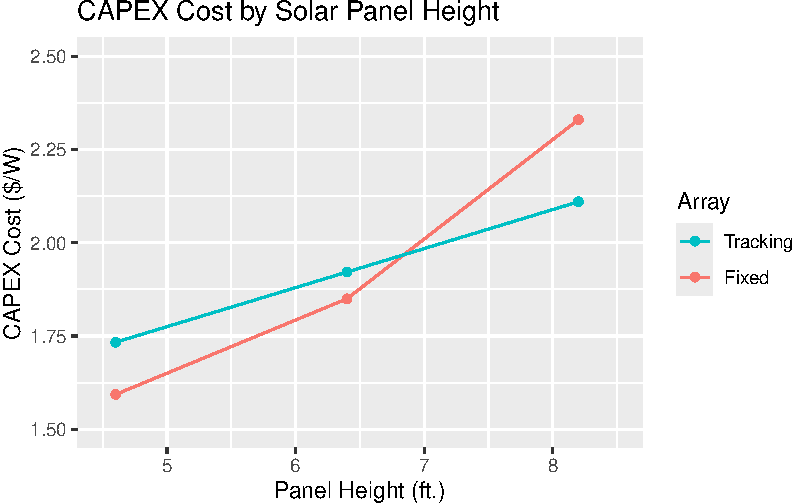
\includegraphics{Simulation_files/figure-pdf/unnamed-chunk-13-1.pdf}

\subsection{Panel Configuration}\label{panel-configuration}

\begin{itemize}
\tightlist
\item
  Panel configuration and DV system output (W).
\end{itemize}

\begin{Shaded}
\begin{Highlighting}[]
\NormalTok{panconf }\OtherTok{\textless{}{-}} \FunctionTok{wb\_read}\NormalTok{(}\AttributeTok{file =} \StringTok{"Parameters.xlsx"}\NormalTok{,}
                \AttributeTok{sheet =} \StringTok{"Panel Spacing"}\NormalTok{,}
                \AttributeTok{start\_row =} \DecValTok{2}\NormalTok{,}
                \AttributeTok{start\_col =} \DecValTok{1}\NormalTok{,}
                \AttributeTok{skip\_empty\_rows =} \ConstantTok{TRUE}\NormalTok{,}
                \AttributeTok{skip\_empty\_cols =} \ConstantTok{TRUE}\NormalTok{,}
                \AttributeTok{col\_names =} \ConstantTok{TRUE}\NormalTok{)}
  \CommentTok{\# rename(avtyps = \textasciigrave{}AV Types\textasciigrave{},}
  \CommentTok{\#        item = Item,}
  \CommentTok{\#        cost = \textasciigrave{}Cost ($/W)\textasciigrave{},}
  \CommentTok{\#        height = \textasciigrave{}Panel Height (ft.)\textasciigrave{},}
  \CommentTok{\#        tcost = \textasciigrave{}Total Cost ($/W)\textasciigrave{})}
\FunctionTok{dim}\NormalTok{(panconf)}
\end{Highlighting}
\end{Shaded}

\begin{verbatim}
[1] 21 21
\end{verbatim}

\begin{Shaded}
\begin{Highlighting}[]
\FunctionTok{head}\NormalTok{(panconf)}
\end{Highlighting}
\end{Shaded}

\begin{verbatim}
  Total Area (Acre) Total Area (Sq. Ft.) Solar Proportion
3                 1                43560             1.00
4                 1                43560             0.95
5                 1                43560             0.90
6                 1                43560             0.85
7                 1                43560             0.80
8                 1                43560             0.75
  Solar Proportion Area (Sq. Ft.) Solar Proportion Area (Sq.M.)
3                           43560                      4046.856
4                           41382                      3844.513
5                           39204                      3642.170
6                           37026                      3439.828
7                           34848                      3237.485
8                           32670                      3035.142
  Side Length (ft.) YSide Length (ft.) XSide length (ft.) Panel Length (ft.)
3          208.7103           208.7103           208.7103               7.75
4          208.7103           208.7103           198.2748               7.75
5          208.7103           208.7103           187.8393               7.75
6          208.7103           208.7103           177.4038               7.75
7          208.7103           208.7103           166.9683               7.75
8          208.7103           208.7103           156.5327               7.75
  Row Seperator (ft.) Panel Width(ft.) Panel Area (Sq. ft.) Panels/Row
3                   6              3.5               27.125         59
4                   6              3.5               27.125         59
5                   6              3.5               27.125         59
6                   6              3.5               27.125         59
7                   6              3.5               27.125         59
8                   6              3.5               27.125         59
  Total Rows Total Panels Array Area (Sq. Ft.) Array Area (Sq. M.)
3         15          885             24005.62            2230.195
4         14          826             22405.25            2081.516
5         13          767             20804.88            1932.836
6         12          708             19204.50            1784.156
7         12          708             19204.50            1784.156
8         11          649             17604.12            1635.477
  XSide Open Length (ft) Inter Panel Spacing (ft) Panel Efficienfy
3                     92                        6             0.19
4                    100                        7             0.19
5                    107                        8             0.19
6                    115                       10             0.19
7                    115                       10             0.19
8                    123                       12             0.19
  DC System Size (kW)
3            423.7371
4            395.4880
5            367.2388
6            338.9897
7            338.9897
8            310.7405
\end{verbatim}

\begin{Shaded}
\begin{Highlighting}[]
\FunctionTok{tail}\NormalTok{(panconf)}
\end{Highlighting}
\end{Shaded}

\begin{verbatim}
   Total Area (Acre) Total Area (Sq. Ft.) Solar Proportion
18                 1                43560             0.25
19                 1                43560             0.20
20                 1                43560             0.15
21                 1                43560             0.10
22                 1                43560             0.05
23                 1                43560             0.00
   Solar Proportion Area (Sq. Ft.) Solar Proportion Area (Sq.M.)
18                           10890                     1011.7140
19                            8712                      809.3712
20                            6534                      607.0284
21                            4356                      404.6856
22                            2178                      202.3428
23                               0                        0.0000
   Side Length (ft.) YSide Length (ft.) XSide length (ft.) Panel Length (ft.)
18          208.7103           208.7103           52.17758               7.75
19          208.7103           208.7103           41.74207               7.75
20          208.7103           208.7103           31.30655               7.75
21          208.7103           208.7103           20.87103               7.75
22          208.7103           208.7103           10.43552               7.75
23          208.7103           208.7103            0.00000               7.75
   Row Seperator (ft.) Panel Width(ft.) Panel Area (Sq. ft.) Panels/Row
18                   6              3.5               27.125         59
19                   6              3.5               27.125         59
20                   6              3.5               27.125         59
21                   6              3.5               27.125         59
22                   6              3.5               27.125         59
23                   6              3.5               27.125         59
   Total Rows Total Panels Array Area (Sq. Ft.) Array Area (Sq. M.)
18          3          177             4801.125            446.0391
19          3          177             4801.125            446.0391
20          2          118             3200.750            297.3594
21          1           59             1600.375            148.6797
22          0            0                0.000              0.0000
23          0            0                0.000              0.0000
   XSide Open Length (ft) Inter Panel Spacing (ft) Panel Efficienfy
18                    185                       92             0.19
19                    185                       92             0.19
20                    193                      193             0.19
21                    200                       NA             0.19
22                    208                       NA             0.19
23                    208                       NA             0.19
   DC System Size (kW)
18            84.74742
19            84.74742
20            56.49828
21            28.24914
22             0.00000
23             0.00000
\end{verbatim}

\subsection{Energy output}\label{energy-output}

Energy output was simulated using NREL
\href{https://pvwatts.nrel.gov/pvwatts.php}{PV Watts Calculator}.

\begin{itemize}
\item
  sprop = land proportion covered by solar in 1 acres. Value ranges from
  0 to 1.
\item
  Panels = Total number of panels in 1 acres of land.
\item
  datalot: 1 = first simulation done for four regions of AL; 2 = second
  simulation done for four regions of AL. Two simulations have two
  unique zipcodes for each simulated region.
\item
  al\_regs = regions of Alabama
\item
  zips = zipcodes selected from each region of AL for simulation.
\item
  array = Fixed (open rack); 1AxisRot = 1 Axis Tracking. See above NREL
  tool for more detail.
\item
  dc\_kw = DC system size, calculated for each solar panel heights
  considering solar panels efficiency and area covered by solar panels.
\item
  energy = total energy output ( kWh/Year) considering system
  parameters. Total hours considered by the model is 8,760 (See
  \href{https://pvwatts.nrel.gov/pvwatts.php}{PV Watts Calculator}
  Results \textgreater{} help (below the result) \textgreater{} results
  \textgreater{} download monthly or hourly results).
\end{itemize}

\begin{Shaded}
\begin{Highlighting}[]
\NormalTok{energy\_output }\OtherTok{\textless{}{-}} \FunctionTok{read\_xlsx}\NormalTok{(}\StringTok{"Parameters.xlsx"}\NormalTok{, }
                           \AttributeTok{sheet =} \StringTok{"Energy Output"}\NormalTok{,}
                           \AttributeTok{start\_row =} \DecValTok{1}\NormalTok{,}
                           \AttributeTok{start\_col =} \DecValTok{1}\NormalTok{,}
                           \AttributeTok{skip\_empty\_rows =} \ConstantTok{TRUE}\NormalTok{,}
                           \AttributeTok{skip\_empty\_cols =} \ConstantTok{TRUE}\NormalTok{,}
                           \AttributeTok{col\_names =} \ConstantTok{TRUE}\NormalTok{) }\SpecialCharTok{\%\textgreater{}\%}
  \FunctionTok{rename}\NormalTok{(}\AttributeTok{sprop =} \StringTok{\textasciigrave{}}\AttributeTok{Solar Proportion}\StringTok{\textasciigrave{}}\NormalTok{,}
         \AttributeTok{panels =} \StringTok{\textasciigrave{}}\AttributeTok{Total Panels}\StringTok{\textasciigrave{}}\NormalTok{,}
         \AttributeTok{datalot =}\NormalTok{ DataLot,}
         \AttributeTok{al\_regs =} \StringTok{\textasciigrave{}}\AttributeTok{Region of AL}\StringTok{\textasciigrave{}}\NormalTok{,}
         \AttributeTok{zips =}\NormalTok{ ZIPCODE,}
         \AttributeTok{array =} \StringTok{\textasciigrave{}}\AttributeTok{Array Type}\StringTok{\textasciigrave{}}\NormalTok{,}
         \AttributeTok{dc\_kw =} \StringTok{\textasciigrave{}}\AttributeTok{DC System Size (kW)}\StringTok{\textasciigrave{}}\NormalTok{,}
         \AttributeTok{energy =} \StringTok{\textasciigrave{}}\AttributeTok{Energy (kWh/Year)}\StringTok{\textasciigrave{}}\NormalTok{) }\SpecialCharTok{\%\textgreater{}\%}
  \FunctionTok{mutate}\NormalTok{(}\AttributeTok{dc\_kw =} \FunctionTok{round}\NormalTok{(dc\_kw, }\DecValTok{2}\NormalTok{),}
         \AttributeTok{array =} \FunctionTok{case\_when}\NormalTok{(}
\NormalTok{           array }\SpecialCharTok{==} \StringTok{"1AxisRot"} \SpecialCharTok{\textasciitilde{}} \StringTok{"Tracking"}\NormalTok{,}
\NormalTok{           array }\SpecialCharTok{==} \StringTok{"FixedOpen"} \SpecialCharTok{\textasciitilde{}} \StringTok{"Fixed"}\NormalTok{,}
           \ConstantTok{TRUE} \SpecialCharTok{\textasciitilde{}}\NormalTok{ array))}

\FunctionTok{dim}\NormalTok{(energy\_output)}
\end{Highlighting}
\end{Shaded}

\begin{verbatim}
[1] 336   8
\end{verbatim}

\begin{Shaded}
\begin{Highlighting}[]
\FunctionTok{head}\NormalTok{(energy\_output)}
\end{Highlighting}
\end{Shaded}

\begin{verbatim}
  sprop panels datalot    al_regs  zips    array  dc_kw energy
2  1.00    885       1   Northern 35801 Tracking 423.74 672887
3  0.95    826       1   Northern 35801 Tracking 395.49 628029
4  0.90    767       1   Northern 35801 Tracking 367.24 583171
5  0.75    649       1 Black Belt 36117 Tracking 310.74 534002
6  0.75    649       2 Black Belt 36040 Tracking 310.74 515824
7  0.80    708       1 Black Belt 36117 Tracking 338.99 582547
\end{verbatim}

\begin{Shaded}
\begin{Highlighting}[]
\FunctionTok{tail}\NormalTok{(energy\_output)}
\end{Highlighting}
\end{Shaded}

\begin{verbatim}
    sprop panels datalot  al_regs  zips array dc_kw energy
332  0.25    177       2 Southern 36507 Fixed 84.75 122697
333  0.20    177       2 Southern 36507 Fixed 84.75 122697
334  0.15    118       2 Southern 36507 Fixed 56.50  81800
335  0.10     59       2 Southern 36507 Fixed 28.25  40902
336  0.05      0       2 Southern 36507 Fixed  0.00      0
337  0.00      0       2 Southern 36507 Fixed  0.00      0
\end{verbatim}

\subsubsection{Energy output by solar panels
counts}\label{energy-output-by-solar-panels-counts}

Plotting Energy output by number of solar panels in one acres of AV
system from fixed and single axis rotation system for two zipcodes (1,
2) within each of the four regions of AL.

\begin{Shaded}
\begin{Highlighting}[]
\NormalTok{lox }\OtherTok{\textless{}{-}} \FunctionTok{c}\NormalTok{(}\StringTok{"Northern"}\NormalTok{, }\StringTok{"Central"}\NormalTok{, }\StringTok{"Black Belt"}\NormalTok{, }\StringTok{"Southern"}\NormalTok{)}
\NormalTok{array\_levs }\OtherTok{=} \FunctionTok{c}\NormalTok{(}\StringTok{"Single Axis Rotation"}\NormalTok{, }\StringTok{"Fixed Open Rack"}\NormalTok{)}
\NormalTok{datalot\_levs }\OtherTok{=} \FunctionTok{c}\NormalTok{(}\StringTok{"Location 1"}\NormalTok{, }\StringTok{"Location 2"}\NormalTok{)}
\FunctionTok{ggplot}\NormalTok{(}\AttributeTok{data =}\NormalTok{ energy\_output,}
         \AttributeTok{mapping =} \FunctionTok{aes}\NormalTok{(}\AttributeTok{x =}\NormalTok{ al\_regs,}
                       \AttributeTok{y =}\NormalTok{ energy,}
                       \CommentTok{\#fill = energy,}
                       \AttributeTok{color =} \FunctionTok{factor}\NormalTok{(panels),}
                       \AttributeTok{group =} \FunctionTok{factor}\NormalTok{(panels))) }\SpecialCharTok{+}
  \FunctionTok{geom\_line}\NormalTok{()}\SpecialCharTok{+}
  \FunctionTok{geom\_point}\NormalTok{() }\SpecialCharTok{+}
  \FunctionTok{facet\_grid}\NormalTok{(datalot}\SpecialCharTok{\textasciitilde{}}\NormalTok{array) }\SpecialCharTok{+}
  \FunctionTok{scale\_x\_discrete}\NormalTok{(}\AttributeTok{limits =}\NormalTok{ lox,}
                   \AttributeTok{labels =} \FunctionTok{c}\NormalTok{(}\StringTok{"North"}\NormalTok{, }\StringTok{"Center"}\NormalTok{, }\StringTok{"B Belt"}\NormalTok{, }\StringTok{"South"}\NormalTok{)) }\SpecialCharTok{+}
  \FunctionTok{guides}\NormalTok{(}\AttributeTok{color =} \FunctionTok{guide\_legend}\NormalTok{(}\AttributeTok{ncol =} \DecValTok{2}\NormalTok{, }\AttributeTok{reverse =} \ConstantTok{TRUE}\NormalTok{))}
\end{Highlighting}
\end{Shaded}

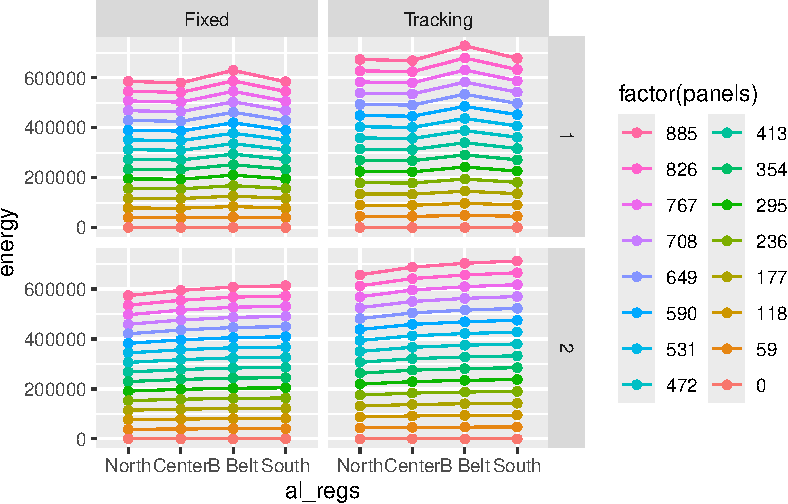
\includegraphics{Simulation_files/figure-pdf/unnamed-chunk-16-1.pdf}

\subsubsection{Energy output by DC System
Size}\label{energy-output-by-dc-system-size}

Plotting Energy output by DC System Size from fixed and single axis
rotation system for two zipcodes (1, 2) within each of the four regions
of AL.

\begin{Shaded}
\begin{Highlighting}[]
\NormalTok{lox }\OtherTok{\textless{}{-}} \FunctionTok{c}\NormalTok{(}\StringTok{"Northern"}\NormalTok{, }\StringTok{"Central"}\NormalTok{, }\StringTok{"Black Belt"}\NormalTok{, }\StringTok{"Southern"}\NormalTok{)}
\FunctionTok{ggplot}\NormalTok{(}\AttributeTok{data =}\NormalTok{ energy\_output,}
         \AttributeTok{mapping =} \FunctionTok{aes}\NormalTok{(}\AttributeTok{x =}\NormalTok{ al\_regs,}
                       \AttributeTok{y =}\NormalTok{ energy,}
                       \CommentTok{\#fill = energy,}
                       \AttributeTok{color =} \FunctionTok{factor}\NormalTok{(dc\_kw),}
                       \AttributeTok{group =} \FunctionTok{factor}\NormalTok{(dc\_kw))) }\SpecialCharTok{+}
  \FunctionTok{geom\_line}\NormalTok{()}\SpecialCharTok{+}
  \FunctionTok{geom\_point}\NormalTok{() }\SpecialCharTok{+}
  \FunctionTok{facet\_grid}\NormalTok{(datalot}\SpecialCharTok{\textasciitilde{}}\NormalTok{array) }\SpecialCharTok{+}
  \FunctionTok{scale\_x\_discrete}\NormalTok{(}\AttributeTok{limits =}\NormalTok{ lox,}
                   \AttributeTok{labels =} \FunctionTok{c}\NormalTok{(}\StringTok{"North"}\NormalTok{, }\StringTok{"Center"}\NormalTok{, }\StringTok{"B Belt"}\NormalTok{, }\StringTok{"South"}\NormalTok{)) }\SpecialCharTok{+}
  \FunctionTok{guides}\NormalTok{(}\AttributeTok{color =} \FunctionTok{guide\_legend}\NormalTok{(}\AttributeTok{ncol =}\DecValTok{2}\NormalTok{, }\AttributeTok{reverse =} \ConstantTok{TRUE}\NormalTok{))}
\end{Highlighting}
\end{Shaded}

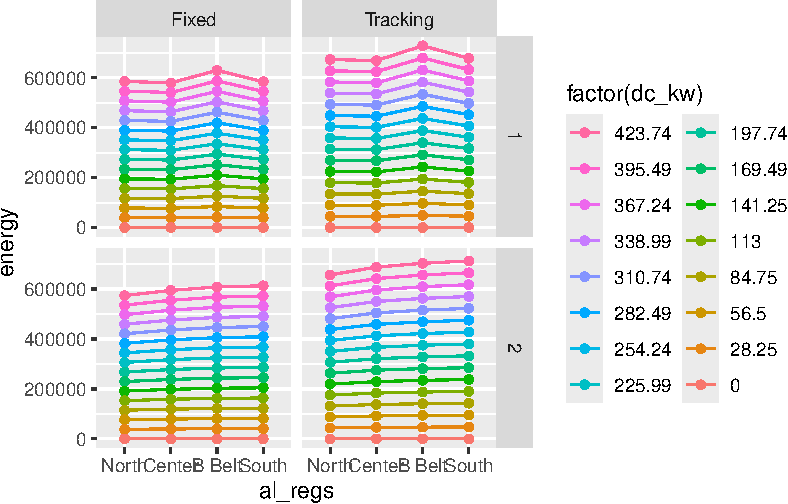
\includegraphics{Simulation_files/figure-pdf/unnamed-chunk-17-1.pdf}

\section{Solar Energy Calculation}\label{solar-energy-calculation}

\subsection{Simulation 1 for energy
revenue}\label{simulation-1-for-energy-revenue}

\begin{itemize}
\item
  elcprc = electricity price. See Electricity price data for more
  detail.
\item
  elcrev = Revenue from electricity for given electricity prices. See
  ``energy output'' and ``electricity price'' dataset for more details.
\item
  I took average of ``energy'' from datalot 1 and datalot 2 to minimize
  computation time.
\end{itemize}

\begin{Shaded}
\begin{Highlighting}[]
\CommentTok{\# Convert to data frames if they are not already}
\NormalTok{matrix1 }\OtherTok{\textless{}{-}}\NormalTok{ energy\_output  }\SpecialCharTok{\%\textgreater{}\%}
  \FunctionTok{group\_by}\NormalTok{(sprop, al\_regs, array, dc\_kw, panels) }\SpecialCharTok{\%\textgreater{}\%}
  \CommentTok{\#filter(datalot == 2) \%\textgreater{}\%}
  \CommentTok{\# Compute mean of datalot 1 and datalot 2:}
  \FunctionTok{summarise}\NormalTok{(}
    \AttributeTok{energy =} \FunctionTok{mean}\NormalTok{(energy),}
    \AttributeTok{.groups =} \StringTok{\textquotesingle{}drop\textquotesingle{}}
\NormalTok{    ) }\CommentTok{\# dimension of matrix is 168*6}
\NormalTok{matrix2 }\OtherTok{\textless{}{-}}\NormalTok{ elec\_price }\CommentTok{\# dimension of matrix is 11*1}

\CommentTok{\# Initialize the result data frame}
\CommentTok{\# energy\_revenue \textless{}{-} data.frame(matrix(nrow = 1848, ncol = 9))}
\NormalTok{energy\_revenue }\OtherTok{\textless{}{-}} \FunctionTok{data.frame}\NormalTok{(}
  \FunctionTok{matrix}\NormalTok{(}\AttributeTok{nrow =} \FunctionTok{nrow}\NormalTok{(matrix2)}\SpecialCharTok{*}\FunctionTok{nrow}\NormalTok{(matrix1),}
         \AttributeTok{ncol =} \FunctionTok{ncol}\NormalTok{(matrix2)}\SpecialCharTok{+}\FunctionTok{ncol}\NormalTok{(matrix1)}\SpecialCharTok{+}\DecValTok{1}\NormalTok{))}

\CommentTok{\# Variable to keep track of the row index in the result matrix}
\NormalTok{row\_index }\OtherTok{\textless{}{-}} \DecValTok{1}

\CommentTok{\# Loop through each value of the second matrix}
\ControlFlowTok{for}\NormalTok{ (i }\ControlFlowTok{in} \DecValTok{1}\SpecialCharTok{:}\FunctionTok{nrow}\NormalTok{(matrix2)) \{}
  \CommentTok{\# Loop through each value of the second matrix}
  \ControlFlowTok{for}\NormalTok{ (j }\ControlFlowTok{in} \DecValTok{1}\SpecialCharTok{:}\FunctionTok{nrow}\NormalTok{(matrix1)) \{}
    \CommentTok{\# First matrix, second matrix, combined two matrices.}
\NormalTok{    new\_row }\OtherTok{\textless{}{-}} \FunctionTok{c}\NormalTok{(matrix1[j, ], }
\NormalTok{                 matrix2[i, ], }
\NormalTok{                 matrix1}\SpecialCharTok{$}\NormalTok{energy[j] }\SpecialCharTok{*}\NormalTok{ matrix2}\SpecialCharTok{$}\NormalTok{epr\_kwh[i])}
    \CommentTok{\# Assign the new row to the result matrix}
\NormalTok{    energy\_revenue[row\_index, ] }\OtherTok{\textless{}{-}}\NormalTok{ new\_row}
    \CommentTok{\# Increment the row index}
\NormalTok{    row\_index }\OtherTok{\textless{}{-}}\NormalTok{ row\_index }\SpecialCharTok{+} \DecValTok{1}
\NormalTok{  \}}
\NormalTok{\}}
\CommentTok{\# Name the columns}
\FunctionTok{colnames}\NormalTok{(energy\_revenue) }\OtherTok{\textless{}{-}} \FunctionTok{c}\NormalTok{(}\FunctionTok{colnames}\NormalTok{(matrix1), }\StringTok{"elcprc"}\NormalTok{, }\StringTok{"elcrev"}\NormalTok{)}

\CommentTok{\# Display the result}
\FunctionTok{dim}\NormalTok{(energy\_revenue)}
\end{Highlighting}
\end{Shaded}

\begin{verbatim}
[1] 1848    8
\end{verbatim}

\begin{Shaded}
\begin{Highlighting}[]
\FunctionTok{head}\NormalTok{(energy\_revenue); }\FunctionTok{tail}\NormalTok{(energy\_revenue)}
\end{Highlighting}
\end{Shaded}

\begin{verbatim}
  sprop    al_regs    array dc_kw panels energy elcprc elcrev
1     0 Black Belt    Fixed     0      0      0   0.01      0
2     0 Black Belt Tracking     0      0      0   0.01      0
3     0    Central    Fixed     0      0      0   0.01      0
4     0    Central Tracking     0      0      0   0.01      0
5     0   Northern    Fixed     0      0      0   0.01      0
6     0   Northern Tracking     0      0      0   0.01      0
\end{verbatim}

\begin{verbatim}
     sprop  al_regs    array  dc_kw panels   energy elcprc   elcrev
1843     1  Central    Fixed 423.74    885 587291.0   0.06 35237.46
1844     1  Central Tracking 423.74    885 678466.0   0.06 40707.96
1845     1 Northern    Fixed 423.74    885 579622.5   0.06 34777.35
1846     1 Northern Tracking 423.74    885 664888.0   0.06 39893.28
1847     1 Southern    Fixed 423.74    885 598720.5   0.06 35923.23
1848     1 Southern Tracking 423.74    885 695415.0   0.06 41724.90
\end{verbatim}

\begin{Shaded}
\begin{Highlighting}[]
\CommentTok{\# Check for any NAs in the result}
\ControlFlowTok{if}\NormalTok{(}\FunctionTok{any}\NormalTok{(}\FunctionTok{is.na}\NormalTok{(energy\_revenue))) \{}
\NormalTok{  na\_indices }\OtherTok{\textless{}{-}} \FunctionTok{which}\NormalTok{(}\FunctionTok{is.na}\NormalTok{(energy\_revenue), }\AttributeTok{arr.ind =} \ConstantTok{TRUE}\NormalTok{)}
  \FunctionTok{print}\NormalTok{(}\FunctionTok{paste}\NormalTok{(}\StringTok{"NAs found at rows:"}\NormalTok{, }\FunctionTok{unique}\NormalTok{(na\_indices[, }\DecValTok{1}\NormalTok{])))}
\NormalTok{\} }\ControlFlowTok{else}\NormalTok{ \{}
  \FunctionTok{print}\NormalTok{(}\StringTok{"No NAs found in the result data frame."}\NormalTok{)}
\NormalTok{\}}
\end{Highlighting}
\end{Shaded}

\begin{verbatim}
[1] "No NAs found in the result data frame."
\end{verbatim}

\subsection{Simulation 2 for energy
revenue}\label{simulation-2-for-energy-revenue}

This simulation has same result as above (Cross checking above code and
output). Results are suppressed but errors and warnings are not. No
error and no warnings means code is working as it should.

\begin{Shaded}
\begin{Highlighting}[]
\DocumentationTok{\#\# | results=\textquotesingle{}hide\textquotesingle{}}
\CommentTok{\# Sample data}
\FunctionTok{set.seed}\NormalTok{(}\DecValTok{123}\NormalTok{)}
\NormalTok{matrix1 }\OtherTok{\textless{}{-}}\NormalTok{ energy\_output }\CommentTok{\# dimension of matrix is 176*7}
\NormalTok{matrix2 }\OtherTok{\textless{}{-}}\NormalTok{ elec\_price }\CommentTok{\# dimension of matrix is 11*1}

\CommentTok{\# Initializing the result matrix}
\NormalTok{result\_matrix }\OtherTok{\textless{}{-}} \FunctionTok{data.frame}\NormalTok{(}\FunctionTok{matrix}\NormalTok{(}\AttributeTok{ncol =} \FunctionTok{nrow}\NormalTok{(matrix2),}
                                   \AttributeTok{nrow =} \DecValTok{0}\NormalTok{))}
\FunctionTok{colnames}\NormalTok{(result\_matrix) }\OtherTok{\textless{}{-}} \FunctionTok{c}\NormalTok{(}\FunctionTok{colnames}\NormalTok{(matrix1),  }\StringTok{"elcrev"}\NormalTok{, }\StringTok{"elcprc"}\NormalTok{)}

\CommentTok{\# Loop to multiply first and second matrices}
\ControlFlowTok{for}\NormalTok{ (i }\ControlFlowTok{in} \DecValTok{1}\SpecialCharTok{:}\FunctionTok{nrow}\NormalTok{(matrix2)) \{}
\NormalTok{  temp\_matrix }\OtherTok{\textless{}{-}}\NormalTok{ matrix1}
\NormalTok{  temp\_matrix}\SpecialCharTok{$}\NormalTok{E\_Prc }\OtherTok{\textless{}{-}}\NormalTok{ matrix2[i, ]}
\NormalTok{  temp\_matrix}\SpecialCharTok{$}\NormalTok{E\_Rev }\OtherTok{\textless{}{-}}\NormalTok{ matrix1}\SpecialCharTok{$}\NormalTok{energy[j] }\SpecialCharTok{*}\NormalTok{ matrix2}\SpecialCharTok{$}\NormalTok{epr\_kwh[i]}
\NormalTok{  result\_matrix }\OtherTok{\textless{}{-}} \FunctionTok{rbind}\NormalTok{(result\_matrix, temp\_matrix)}
\NormalTok{\}}

\CommentTok{\# Display the resulting matrix}
\FunctionTok{dim}\NormalTok{(result\_matrix)}
\FunctionTok{head}\NormalTok{(result\_matrix)}
\FunctionTok{tail}\NormalTok{(result\_matrix)}
\end{Highlighting}
\end{Shaded}

\subsection{Plotting revenue from energy
production}\label{plotting-revenue-from-energy-production}

\subsubsection{Breakdown by number of solar
panels}\label{breakdown-by-number-of-solar-panels}

I am using data from simulation 1 for this visualization. This code
plots one chart per electricity cost. There are 11 electricity cost
resulting into 11 charts. Electricity revenue is average revenue of
first and second lots of simulation.

\begin{Shaded}
\begin{Highlighting}[]
\NormalTok{lox }\OtherTok{\textless{}{-}} \FunctionTok{c}\NormalTok{(}\StringTok{"Northern"}\NormalTok{, }\StringTok{"Central"}\NormalTok{, }\StringTok{"Black Belt"}\NormalTok{, }\StringTok{"Southern"}\NormalTok{)}
\NormalTok{array\_levs }\OtherTok{=} \FunctionTok{c}\NormalTok{(}\StringTok{"Single Axis Rotation"}\NormalTok{, }\StringTok{"Fixed Open Rack"}\NormalTok{)}
\NormalTok{datalot\_levs }\OtherTok{=} \FunctionTok{c}\NormalTok{(}\StringTok{"Location 1"}\NormalTok{, }\StringTok{"Location 2"}\NormalTok{)}
\ControlFlowTok{for}\NormalTok{ (i }\ControlFlowTok{in} \FunctionTok{unique}\NormalTok{(energy\_revenue}\SpecialCharTok{$}\NormalTok{elcprc)) \{}
\NormalTok{ a }\OtherTok{=} \FunctionTok{ggplot}\NormalTok{(}\AttributeTok{data =}\NormalTok{ (energy\_revenue }\SpecialCharTok{\%\textgreater{}\%}
  \FunctionTok{filter}\NormalTok{(elcprc }\SpecialCharTok{==}\NormalTok{ i)),}
         \AttributeTok{mapping =} \FunctionTok{aes}\NormalTok{(}\AttributeTok{x =}\NormalTok{al\_regs,}
                       \AttributeTok{y =}\NormalTok{ elcrev,}
                       \CommentTok{\#fill = energy,}
                       \AttributeTok{color =} \FunctionTok{factor}\NormalTok{(panels),}
                       \AttributeTok{group =} \FunctionTok{factor}\NormalTok{(panels)))}\SpecialCharTok{+}
  \FunctionTok{geom\_line}\NormalTok{()}\SpecialCharTok{+}
  \FunctionTok{geom\_point}\NormalTok{()}\SpecialCharTok{+}
  \FunctionTok{facet\_grid}\NormalTok{(.}\SpecialCharTok{\textasciitilde{}}\NormalTok{array) }\SpecialCharTok{+}
  \FunctionTok{scale\_x\_discrete}\NormalTok{(}\AttributeTok{limits =}\NormalTok{ lox,}
                   \AttributeTok{labels =} \FunctionTok{c}\NormalTok{(}\StringTok{"North"}\NormalTok{, }\StringTok{"Center"}\NormalTok{, }\StringTok{"B Belt"}\NormalTok{, }\StringTok{"South"}\NormalTok{)) }\SpecialCharTok{+}
   \FunctionTok{guides}\NormalTok{(}\AttributeTok{color =} \FunctionTok{guide\_legend}\NormalTok{(}\AttributeTok{ncol =}\DecValTok{2}\NormalTok{, }\AttributeTok{reverse =} \ConstantTok{TRUE}\NormalTok{))}
 \FunctionTok{cat}\NormalTok{(}\StringTok{"Electricity Price = "}\NormalTok{, i)}
 \FunctionTok{print}\NormalTok{(a)}
\NormalTok{\}}
\end{Highlighting}
\end{Shaded}

\begin{verbatim}
Electricity Price =  0.01
\end{verbatim}

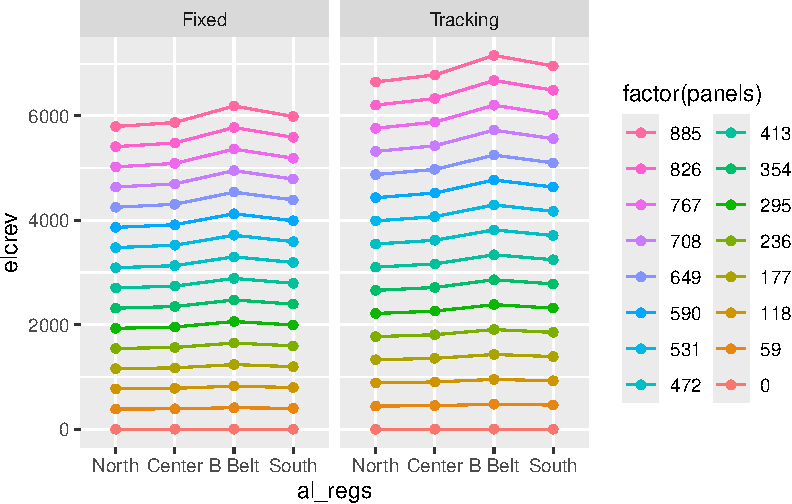
\includegraphics{Simulation_files/figure-pdf/unnamed-chunk-20-1.pdf}

\begin{verbatim}
Electricity Price =  0.015
\end{verbatim}

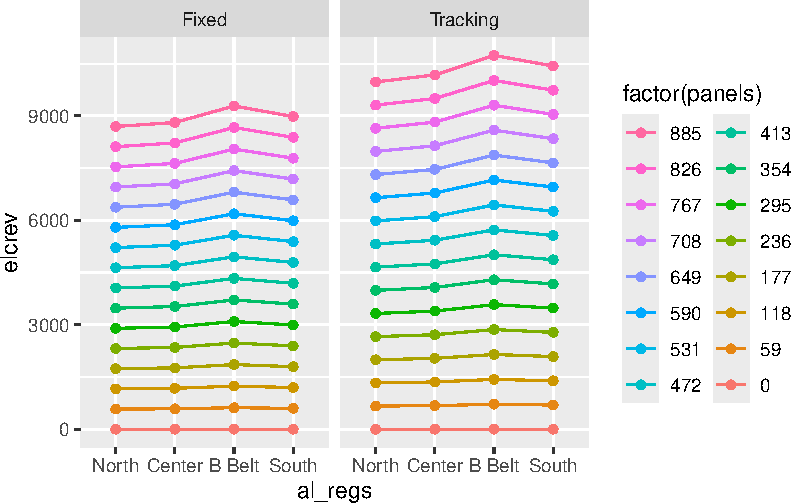
\includegraphics{Simulation_files/figure-pdf/unnamed-chunk-20-2.pdf}

\begin{verbatim}
Electricity Price =  0.02
\end{verbatim}

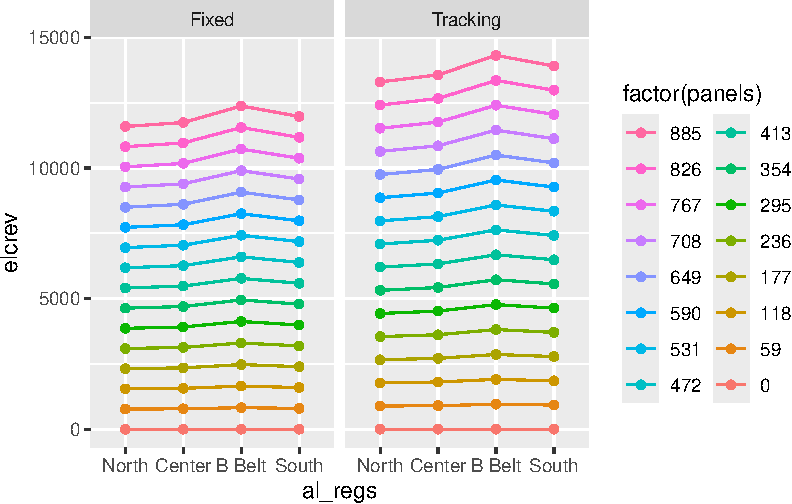
\includegraphics{Simulation_files/figure-pdf/unnamed-chunk-20-3.pdf}

\begin{verbatim}
Electricity Price =  0.025
\end{verbatim}

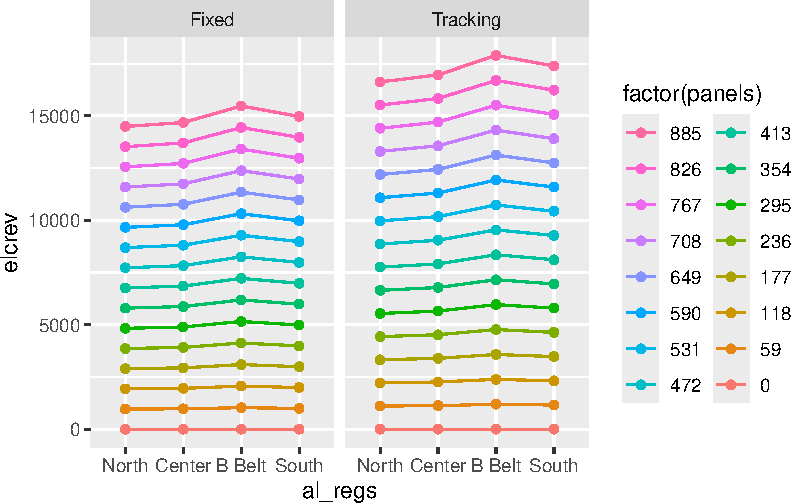
\includegraphics{Simulation_files/figure-pdf/unnamed-chunk-20-4.pdf}

\begin{verbatim}
Electricity Price =  0.03
\end{verbatim}

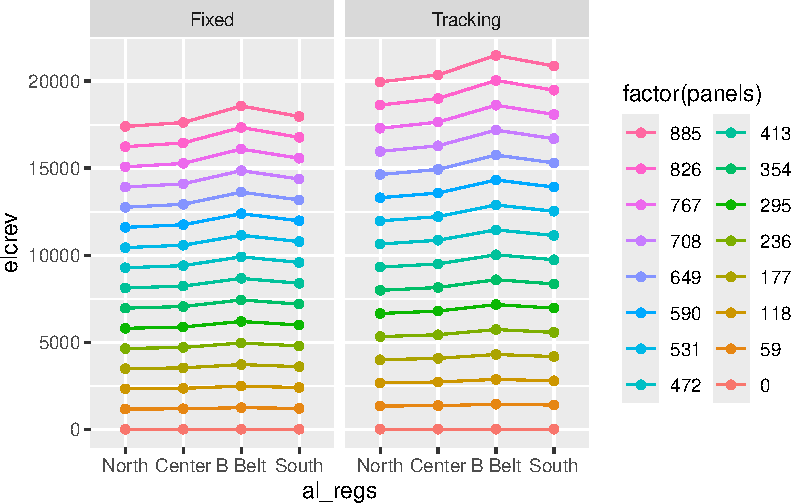
\includegraphics{Simulation_files/figure-pdf/unnamed-chunk-20-5.pdf}

\begin{verbatim}
Electricity Price =  0.035
\end{verbatim}

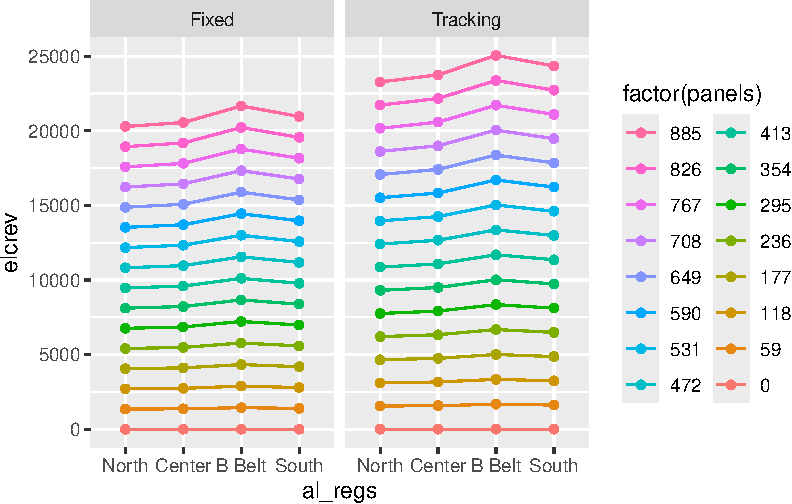
\includegraphics{Simulation_files/figure-pdf/unnamed-chunk-20-6.pdf}

\begin{verbatim}
Electricity Price =  0.04
\end{verbatim}

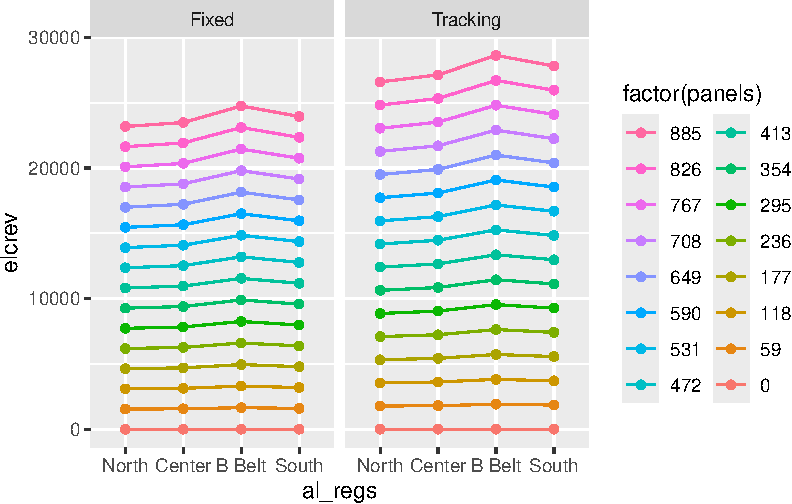
\includegraphics{Simulation_files/figure-pdf/unnamed-chunk-20-7.pdf}

\begin{verbatim}
Electricity Price =  0.045
\end{verbatim}

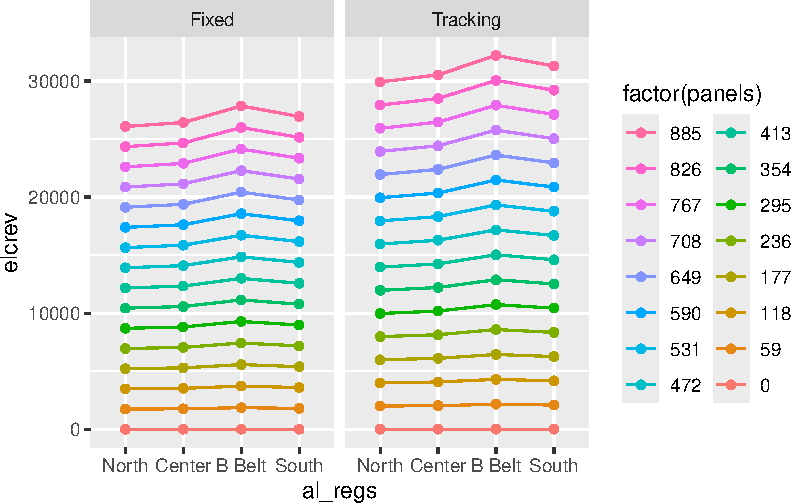
\includegraphics{Simulation_files/figure-pdf/unnamed-chunk-20-8.pdf}

\begin{verbatim}
Electricity Price =  0.05
\end{verbatim}

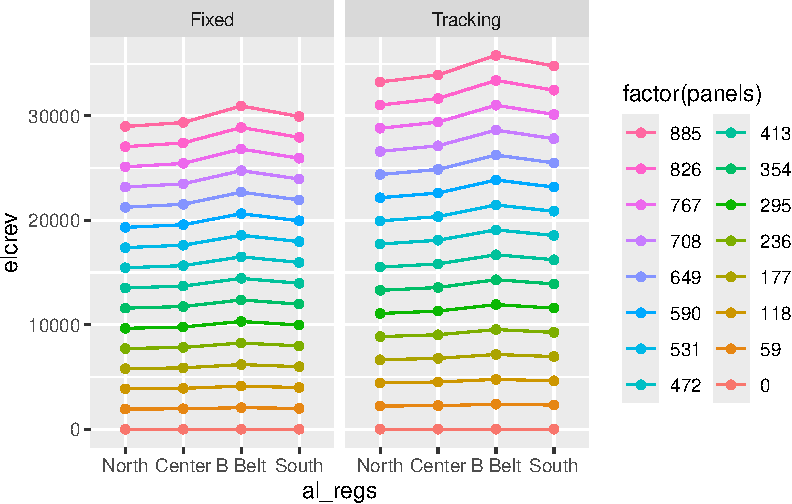
\includegraphics{Simulation_files/figure-pdf/unnamed-chunk-20-9.pdf}

\begin{verbatim}
Electricity Price =  0.055
\end{verbatim}

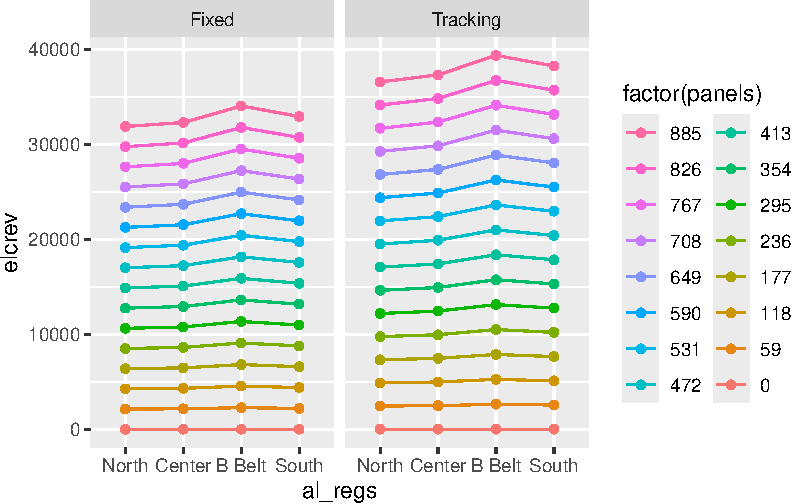
\includegraphics{Simulation_files/figure-pdf/unnamed-chunk-20-10.pdf}

\begin{verbatim}
Electricity Price =  0.06
\end{verbatim}

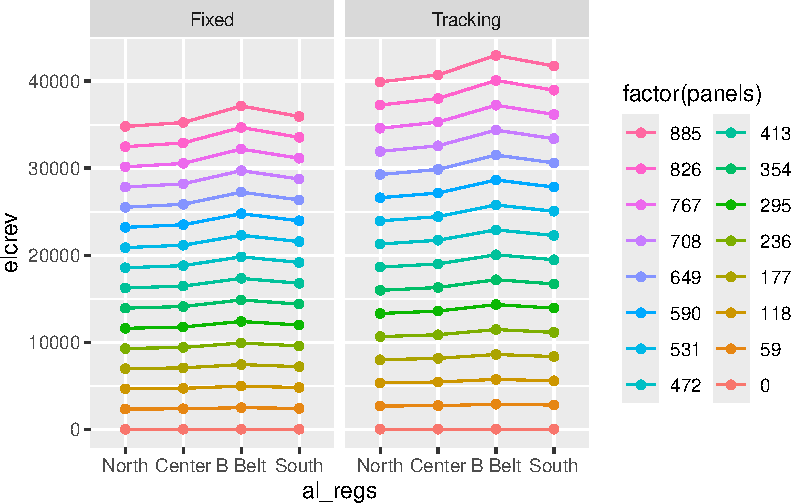
\includegraphics{Simulation_files/figure-pdf/unnamed-chunk-20-11.pdf}

\subsubsection{Breakdown by proportion of land under solar
panels}\label{breakdown-by-proportion-of-land-under-solar-panels}

\begin{itemize}
\tightlist
\item
  Two proportions may have same number of solar panels (Eg. 0.80 and
  0.85, 0.20 and 0.25). So, total lines in the chart may not match with
  total number of legend levels. Some proportions are overlapping in the
  chart. See panel configuration for more detail.
\end{itemize}

\begin{Shaded}
\begin{Highlighting}[]
\NormalTok{lox }\OtherTok{\textless{}{-}} \FunctionTok{c}\NormalTok{(}\StringTok{"Northern"}\NormalTok{, }\StringTok{"Central"}\NormalTok{, }\StringTok{"Black Belt"}\NormalTok{, }\StringTok{"Southern"}\NormalTok{)}
\NormalTok{array\_levs }\OtherTok{=} \FunctionTok{c}\NormalTok{(}\StringTok{"Single Axis Rotation"}\NormalTok{, }\StringTok{"Fixed Open Rack"}\NormalTok{)}
\NormalTok{datalot\_levs }\OtherTok{=} \FunctionTok{c}\NormalTok{(}\StringTok{"Location 1"}\NormalTok{, }\StringTok{"Location 2"}\NormalTok{)}
\ControlFlowTok{for}\NormalTok{ (i }\ControlFlowTok{in} \FunctionTok{unique}\NormalTok{(energy\_revenue}\SpecialCharTok{$}\NormalTok{elcprc)) \{}
\NormalTok{ a }\OtherTok{=} \FunctionTok{ggplot}\NormalTok{(}\AttributeTok{data =}\NormalTok{ (energy\_revenue }\SpecialCharTok{\%\textgreater{}\%}
  \FunctionTok{filter}\NormalTok{(elcprc }\SpecialCharTok{==}\NormalTok{ i)),}
         \AttributeTok{mapping =} \FunctionTok{aes}\NormalTok{(}\AttributeTok{x =}\NormalTok{al\_regs,}
                       \AttributeTok{y =}\NormalTok{ elcrev,}
                       \CommentTok{\#fill = energy,}
                       \AttributeTok{color =} \FunctionTok{factor}\NormalTok{(sprop),}
                       \AttributeTok{group =} \FunctionTok{factor}\NormalTok{(sprop)))}\SpecialCharTok{+}
  \FunctionTok{geom\_line}\NormalTok{()}\SpecialCharTok{+}
  \FunctionTok{geom\_point}\NormalTok{()}\SpecialCharTok{+}
  \FunctionTok{facet\_grid}\NormalTok{(.}\SpecialCharTok{\textasciitilde{}}\NormalTok{array) }\SpecialCharTok{+}
  \FunctionTok{scale\_x\_discrete}\NormalTok{(}\AttributeTok{limits =}\NormalTok{ lox,}
                   \AttributeTok{labels =} \FunctionTok{c}\NormalTok{(}\StringTok{"North"}\NormalTok{, }\StringTok{"Center"}\NormalTok{, }\StringTok{"B Belt"}\NormalTok{, }\StringTok{"South"}\NormalTok{)) }\SpecialCharTok{+}
   \FunctionTok{guides}\NormalTok{(}\AttributeTok{color =} \FunctionTok{guide\_legend}\NormalTok{(}\AttributeTok{ncol =} \DecValTok{2}\NormalTok{, }\AttributeTok{reverse =} \ConstantTok{TRUE}\NormalTok{))}
 \FunctionTok{cat}\NormalTok{(}\StringTok{"Electricity Price = "}\NormalTok{, i)}
 \FunctionTok{print}\NormalTok{(a)}
\NormalTok{\}}
\end{Highlighting}
\end{Shaded}

\begin{verbatim}
Electricity Price =  0.01
\end{verbatim}

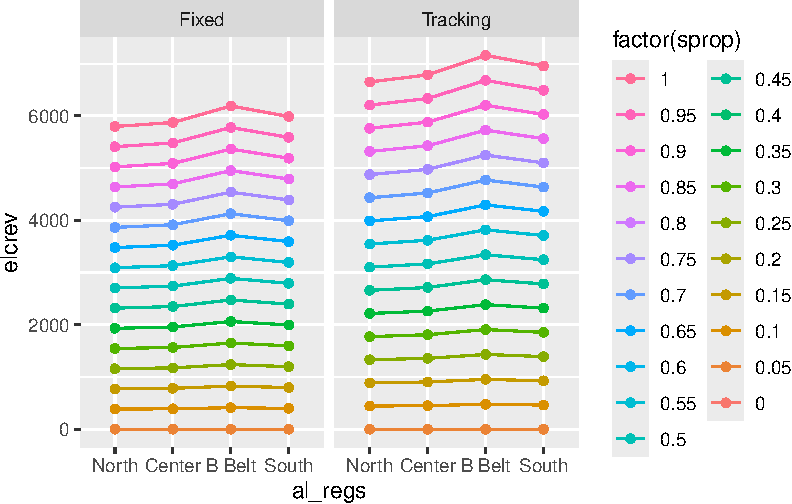
\includegraphics{Simulation_files/figure-pdf/unnamed-chunk-21-1.pdf}

\begin{verbatim}
Electricity Price =  0.015
\end{verbatim}

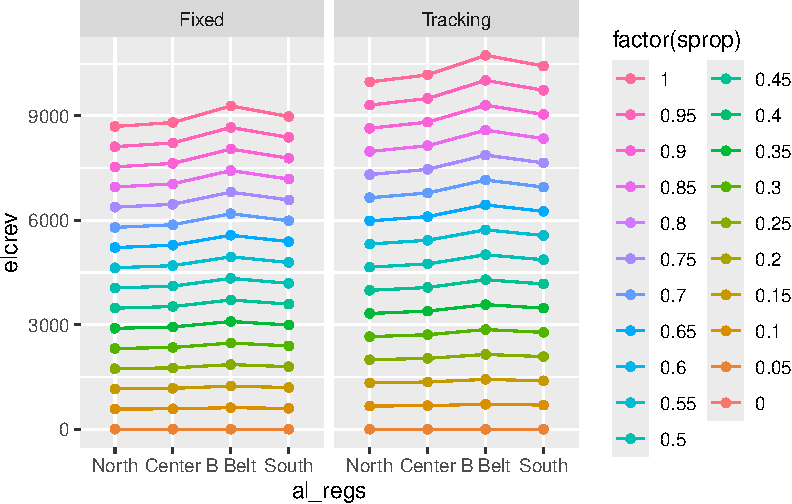
\includegraphics{Simulation_files/figure-pdf/unnamed-chunk-21-2.pdf}

\begin{verbatim}
Electricity Price =  0.02
\end{verbatim}

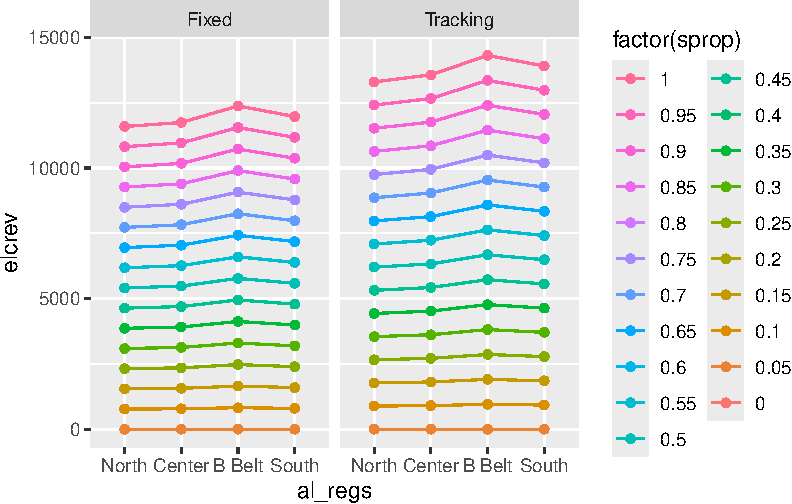
\includegraphics{Simulation_files/figure-pdf/unnamed-chunk-21-3.pdf}

\begin{verbatim}
Electricity Price =  0.025
\end{verbatim}

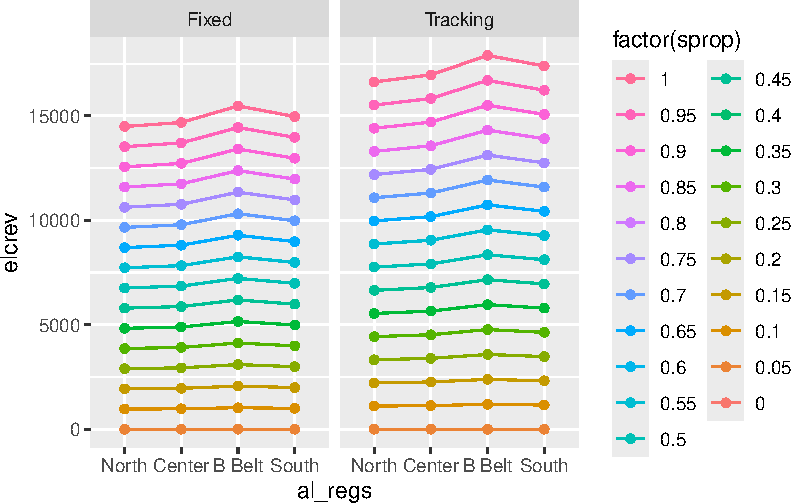
\includegraphics{Simulation_files/figure-pdf/unnamed-chunk-21-4.pdf}

\begin{verbatim}
Electricity Price =  0.03
\end{verbatim}

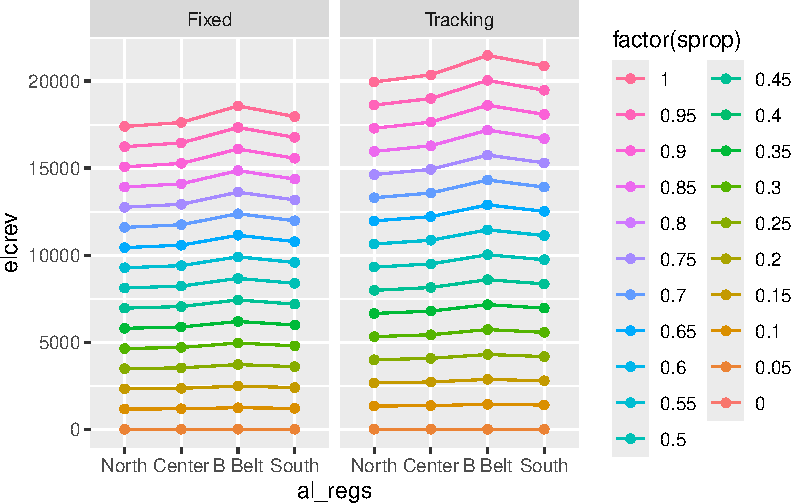
\includegraphics{Simulation_files/figure-pdf/unnamed-chunk-21-5.pdf}

\begin{verbatim}
Electricity Price =  0.035
\end{verbatim}

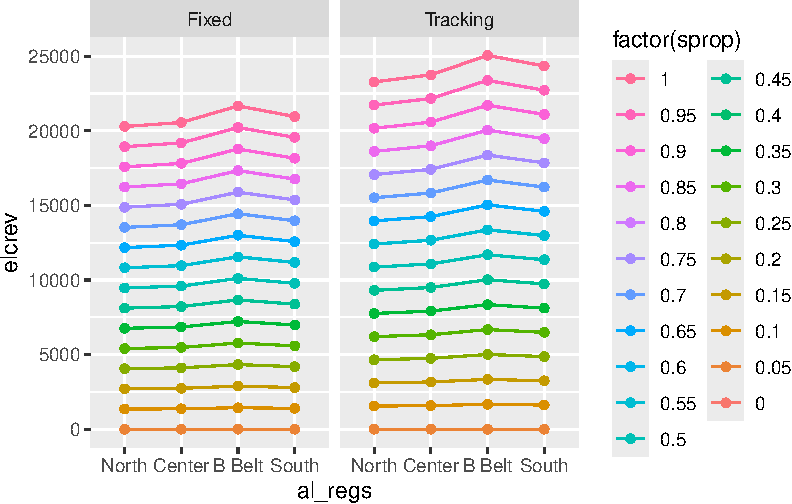
\includegraphics{Simulation_files/figure-pdf/unnamed-chunk-21-6.pdf}

\begin{verbatim}
Electricity Price =  0.04
\end{verbatim}

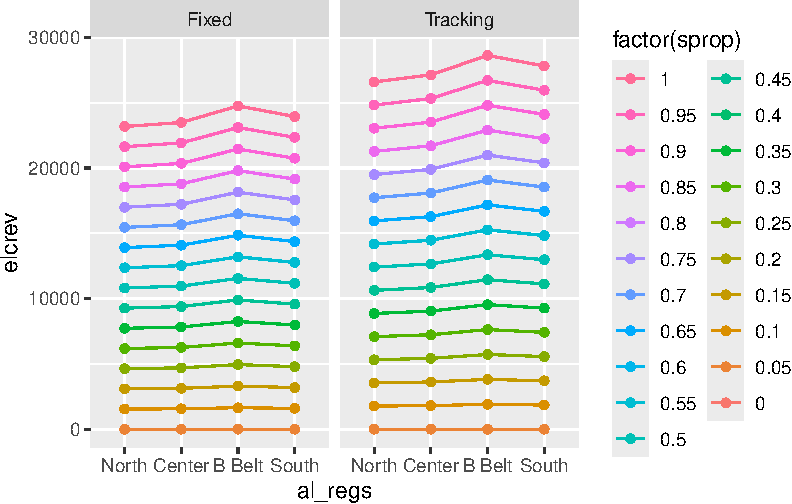
\includegraphics{Simulation_files/figure-pdf/unnamed-chunk-21-7.pdf}

\begin{verbatim}
Electricity Price =  0.045
\end{verbatim}

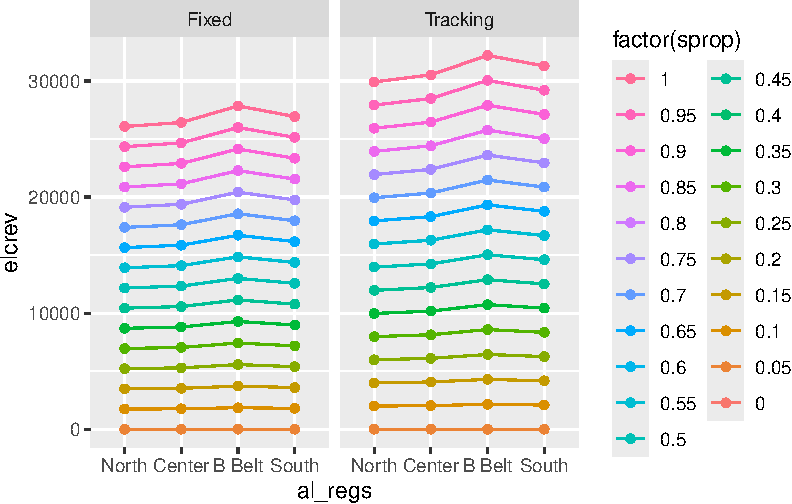
\includegraphics{Simulation_files/figure-pdf/unnamed-chunk-21-8.pdf}

\begin{verbatim}
Electricity Price =  0.05
\end{verbatim}

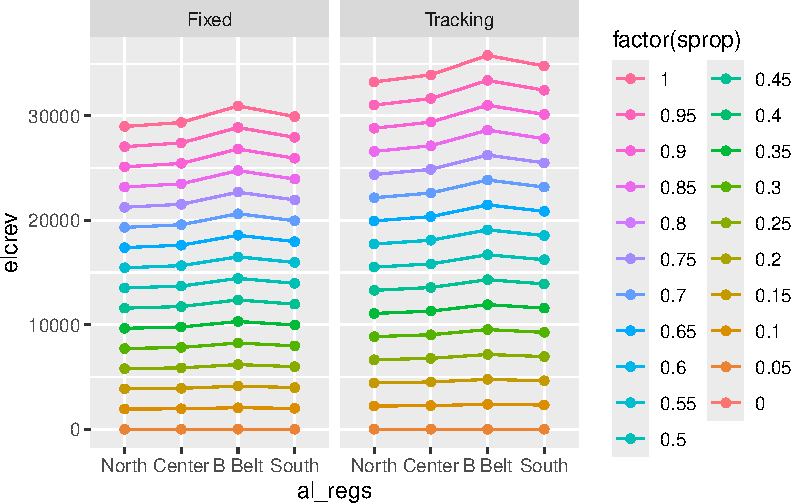
\includegraphics{Simulation_files/figure-pdf/unnamed-chunk-21-9.pdf}

\begin{verbatim}
Electricity Price =  0.055
\end{verbatim}

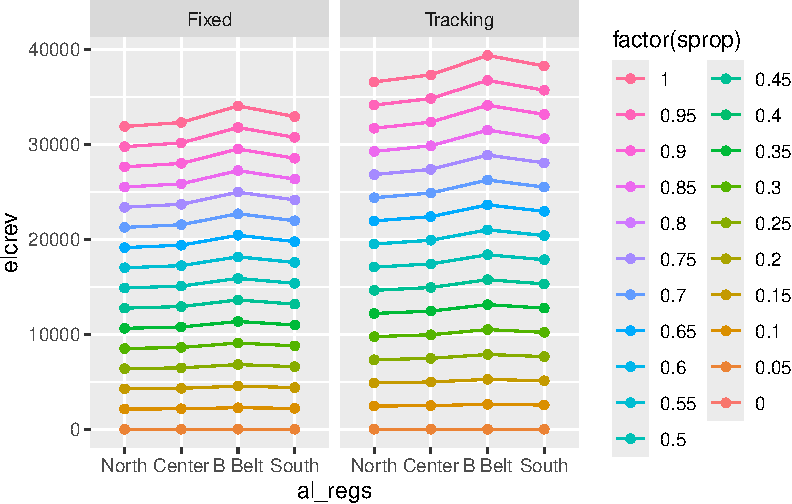
\includegraphics{Simulation_files/figure-pdf/unnamed-chunk-21-10.pdf}

\begin{verbatim}
Electricity Price =  0.06
\end{verbatim}

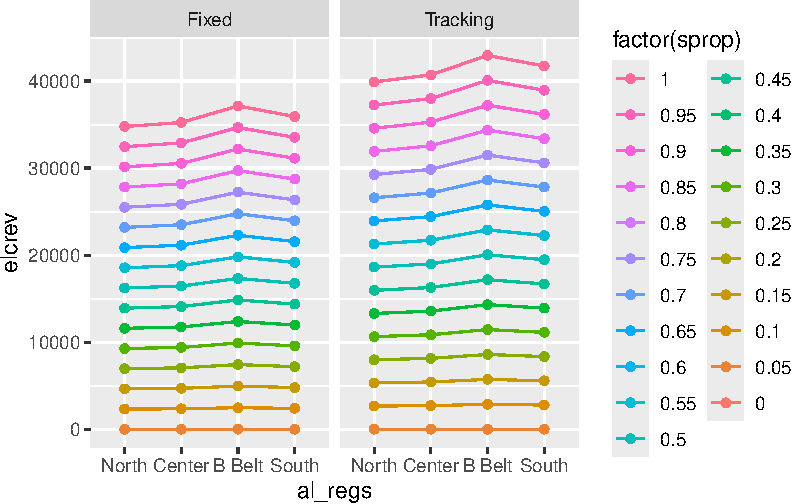
\includegraphics{Simulation_files/figure-pdf/unnamed-chunk-21-11.pdf}

\subsection{Solar system cost}\label{solar-system-cost}

\begin{itemize}
\item
  Cost of solar energy system in agrivoltaic setting.
\item
  I used DC system size (dc\_kw) and capex (\$/w) to get total cost for
  each height and panel tracking system.
\item
  height = height of solar panels; see capex dataset for details.
\item
  capex = capex from capex table; see capex dataset for details.
\item
  ttlcost = Total cost for given DC system size.
\item
  anncost = Annual payment to repay loan (\(P_{ann}\)) =
  \(\frac{P_o(i(1 + i)^t)}{(1+i)^t - 1)}\) , where \(P_o\) = CAPEX loan
  burrowed to repay in \(t\) years; \(t = 25\), and \(i\) = annual
  interest rate at \(5\%\).
\item
  moncost = Monthly payment to repay loan (\(P_{mon}\)) =
  \(\frac{P_o((i/12)(1 + (i/12))^{t*12})}{(1+(i/12))^{t*12} - 1)}\),
  where \(P_o\) = CAPEX loan burrowed to repay in \(t\) years;
  \(t = 25\), and \(i\) = annual interest rate at \(5\%\).
\end{itemize}

\begin{Shaded}
\begin{Highlighting}[]
\NormalTok{expanded\_data }\OtherTok{\textless{}{-}}\NormalTok{ energy\_revenue }\SpecialCharTok{\%\textgreater{}\%}
  \FunctionTok{slice}\NormalTok{(}\FunctionTok{rep}\NormalTok{(}\DecValTok{1}\SpecialCharTok{:}\FunctionTok{n}\NormalTok{(),}
            \AttributeTok{each =} \DecValTok{3}\NormalTok{))}
\NormalTok{capex\_height }\OtherTok{\textless{}{-}} \FunctionTok{rep}\NormalTok{(}\FunctionTok{unique}\NormalTok{(capex}\SpecialCharTok{$}\NormalTok{height),}
                    \AttributeTok{length.out =} \FunctionTok{nrow}\NormalTok{(energy\_revenue))}
\NormalTok{energy\_cost }\OtherTok{=} \FunctionTok{cbind}\NormalTok{(expanded\_data, capex\_height) }\SpecialCharTok{\%\textgreater{}\%} 
  \FunctionTok{rename}\NormalTok{(}\AttributeTok{height =}\NormalTok{ capex\_height)}

\NormalTok{energy\_cost }\OtherTok{\textless{}{-}} \FunctionTok{left\_join}\NormalTok{(energy\_cost, }
\NormalTok{                         capex, }
                         \AttributeTok{by =} \FunctionTok{c}\NormalTok{(}\StringTok{"array"}\NormalTok{, }\StringTok{"height"}\NormalTok{)) }\SpecialCharTok{\%\textgreater{}\%} 
  \FunctionTok{mutate}\NormalTok{(}\AttributeTok{ttlcost =}\NormalTok{ capex}\SpecialCharTok{*}\NormalTok{dc\_kw,}
         \AttributeTok{anncost =}\NormalTok{ ttlcost}\SpecialCharTok{*}\NormalTok{(}\FloatTok{0.05}\SpecialCharTok{*}\NormalTok{(}\DecValTok{1} \SpecialCharTok{+} \FloatTok{0.05}\NormalTok{)}\SpecialCharTok{\^{}}\DecValTok{25}\NormalTok{)}\SpecialCharTok{/}
\NormalTok{           ((}\DecValTok{1} \SpecialCharTok{+} \FloatTok{0.05}\NormalTok{)}\SpecialCharTok{\^{}}\DecValTok{25} \SpecialCharTok{{-}} \DecValTok{1}\NormalTok{),}
         \AttributeTok{moncost =}\NormalTok{ ttlcost}\SpecialCharTok{*}\NormalTok{((}\FloatTok{0.05}\SpecialCharTok{/}\DecValTok{12}\NormalTok{)}\SpecialCharTok{*}\NormalTok{(}\DecValTok{1} \SpecialCharTok{+}\NormalTok{ (}\FloatTok{0.05}\SpecialCharTok{/}\DecValTok{12}\NormalTok{))}\SpecialCharTok{\^{}}\NormalTok{(}\DecValTok{25}\SpecialCharTok{*}\DecValTok{12}\NormalTok{))}\SpecialCharTok{/}
\NormalTok{           ((}\DecValTok{1} \SpecialCharTok{+}\NormalTok{ (}\FloatTok{0.05}\SpecialCharTok{/}\DecValTok{12}\NormalTok{))}\SpecialCharTok{\^{}}\NormalTok{(}\DecValTok{25}\SpecialCharTok{*}\DecValTok{12}\NormalTok{) }\SpecialCharTok{{-}} \DecValTok{1}\NormalTok{))}

\FunctionTok{dim}\NormalTok{(energy\_cost)}
\end{Highlighting}
\end{Shaded}

\begin{verbatim}
[1] 5544   13
\end{verbatim}

\begin{Shaded}
\begin{Highlighting}[]
\FunctionTok{head}\NormalTok{(energy\_cost)}
\end{Highlighting}
\end{Shaded}

\begin{verbatim}
  sprop    al_regs    array dc_kw panels energy elcprc elcrev height    capex
1     0 Black Belt    Fixed     0      0      0   0.01      0    4.6 1.593333
2     0 Black Belt    Fixed     0      0      0   0.01      0    6.4 1.850000
3     0 Black Belt    Fixed     0      0      0   0.01      0    8.2 2.330000
4     0 Black Belt Tracking     0      0      0   0.01      0    4.6 1.733333
5     0 Black Belt Tracking     0      0      0   0.01      0    6.4 1.921667
6     0 Black Belt Tracking     0      0      0   0.01      0    8.2 2.110000
  ttlcost anncost moncost
1       0       0       0
2       0       0       0
3       0       0       0
4       0       0       0
5       0       0       0
6       0       0       0
\end{verbatim}

\begin{Shaded}
\begin{Highlighting}[]
\FunctionTok{tail}\NormalTok{(energy\_cost)}
\end{Highlighting}
\end{Shaded}

\begin{verbatim}
     sprop  al_regs    array  dc_kw panels   energy elcprc   elcrev height
5539     1 Southern    Fixed 423.74    885 598720.5   0.06 35923.23    4.6
5540     1 Southern    Fixed 423.74    885 598720.5   0.06 35923.23    6.4
5541     1 Southern    Fixed 423.74    885 598720.5   0.06 35923.23    8.2
5542     1 Southern Tracking 423.74    885 695415.0   0.06 41724.90    4.6
5543     1 Southern Tracking 423.74    885 695415.0   0.06 41724.90    6.4
5544     1 Southern Tracking 423.74    885 695415.0   0.06 41724.90    8.2
        capex  ttlcost  anncost  moncost
5539 1.593333 675.1591 47.90419 3.946913
5540 1.850000 783.9190 55.62098 4.582712
5541 2.330000 987.3142 70.05237 5.771740
5542 1.733333 734.4827 52.11335 4.293713
5543 1.921667 814.2870 57.77567 4.760241
5544 2.110000 894.0914 63.43798 5.226769
\end{verbatim}

\subsection{Profit from solar}\label{profit-from-solar}

Profit from solar energy system in agrivoltaic setting

\begin{itemize}
\tightlist
\item
  eprofit = profit from electricity after subtracting total cost
  (ttlcost) from total revenue (elcrev).
\item
  eannprof = annual profit from solar after subtracting annual loan
  repayment distributed over 25 years.
\item
  emonprof = monthly profit from solar after subtracting monthly loan
  repayment distributed over 25 years.
\end{itemize}

\begin{Shaded}
\begin{Highlighting}[]
\NormalTok{solar\_profit }\OtherTok{\textless{}{-}}\NormalTok{ energy\_cost }\SpecialCharTok{\%\textgreater{}\%}
  \FunctionTok{mutate}\NormalTok{(}\AttributeTok{eprofit =}\NormalTok{ elcrev }\SpecialCharTok{{-}}\NormalTok{ ttlcost,}
         \AttributeTok{eannprof =}\NormalTok{ elcrev }\SpecialCharTok{{-}}\NormalTok{ anncost,}
         \AttributeTok{emonprof =}\NormalTok{ (elcrev}\SpecialCharTok{/}\DecValTok{12}\NormalTok{) }\SpecialCharTok{{-}}\NormalTok{ moncost)}
\FunctionTok{dim}\NormalTok{(solar\_profit)}
\end{Highlighting}
\end{Shaded}

\begin{verbatim}
[1] 5544   16
\end{verbatim}

\begin{Shaded}
\begin{Highlighting}[]
\FunctionTok{head}\NormalTok{(solar\_profit)}
\end{Highlighting}
\end{Shaded}

\begin{verbatim}
  sprop    al_regs    array dc_kw panels energy elcprc elcrev height    capex
1     0 Black Belt    Fixed     0      0      0   0.01      0    4.6 1.593333
2     0 Black Belt    Fixed     0      0      0   0.01      0    6.4 1.850000
3     0 Black Belt    Fixed     0      0      0   0.01      0    8.2 2.330000
4     0 Black Belt Tracking     0      0      0   0.01      0    4.6 1.733333
5     0 Black Belt Tracking     0      0      0   0.01      0    6.4 1.921667
6     0 Black Belt Tracking     0      0      0   0.01      0    8.2 2.110000
  ttlcost anncost moncost eprofit eannprof emonprof
1       0       0       0       0        0        0
2       0       0       0       0        0        0
3       0       0       0       0        0        0
4       0       0       0       0        0        0
5       0       0       0       0        0        0
6       0       0       0       0        0        0
\end{verbatim}

\begin{Shaded}
\begin{Highlighting}[]
\FunctionTok{tail}\NormalTok{(solar\_profit)}
\end{Highlighting}
\end{Shaded}

\begin{verbatim}
     sprop  al_regs    array  dc_kw panels   energy elcprc   elcrev height
5539     1 Southern    Fixed 423.74    885 598720.5   0.06 35923.23    4.6
5540     1 Southern    Fixed 423.74    885 598720.5   0.06 35923.23    6.4
5541     1 Southern    Fixed 423.74    885 598720.5   0.06 35923.23    8.2
5542     1 Southern Tracking 423.74    885 695415.0   0.06 41724.90    4.6
5543     1 Southern Tracking 423.74    885 695415.0   0.06 41724.90    6.4
5544     1 Southern Tracking 423.74    885 695415.0   0.06 41724.90    8.2
        capex  ttlcost  anncost  moncost  eprofit eannprof emonprof
5539 1.593333 675.1591 47.90419 3.946913 35248.07 35875.33 2989.656
5540 1.850000 783.9190 55.62098 4.582712 35139.31 35867.61 2989.020
5541 2.330000 987.3142 70.05237 5.771740 34935.92 35853.18 2987.831
5542 1.733333 734.4827 52.11335 4.293713 40990.42 41672.79 3472.781
5543 1.921667 814.2870 57.77567 4.760241 40910.61 41667.12 3472.315
5544 2.110000 894.0914 63.43798 5.226769 40830.81 41661.46 3471.848
\end{verbatim}

\subsubsection{Plot profit from solar}\label{plot-profit-from-solar}

\begin{Shaded}
\begin{Highlighting}[]
\NormalTok{lox }\OtherTok{\textless{}{-}} \FunctionTok{c}\NormalTok{(}\StringTok{"Northern"}\NormalTok{, }\StringTok{"Central"}\NormalTok{, }\StringTok{"Black Belt"}\NormalTok{, }\StringTok{"Southern"}\NormalTok{)}
\NormalTok{array\_levs }\OtherTok{=} \FunctionTok{c}\NormalTok{(}\StringTok{"Single Axis Rotation"}\NormalTok{, }\StringTok{"Fixed Open Rack"}\NormalTok{)}
\NormalTok{datalot\_levs }\OtherTok{=} \FunctionTok{c}\NormalTok{(}\StringTok{"Location 1"}\NormalTok{, }\StringTok{"Location 2"}\NormalTok{)}
  \ControlFlowTok{for}\NormalTok{ (i }\ControlFlowTok{in} \FunctionTok{unique}\NormalTok{(solar\_profit}\SpecialCharTok{$}\NormalTok{elcprc)) \{}
\NormalTok{    b }\OtherTok{=} \FunctionTok{ggplot}\NormalTok{(}
      \AttributeTok{data =}\NormalTok{ (solar\_profit }\SpecialCharTok{\%\textgreater{}\%}
                \FunctionTok{filter}\NormalTok{(elcprc }\SpecialCharTok{==}\NormalTok{ i)),}
      \AttributeTok{mapping =} \FunctionTok{aes}\NormalTok{(}
        \AttributeTok{x =}\NormalTok{ al\_regs,}
        \AttributeTok{y =}\NormalTok{ eprofit,}
        \CommentTok{\#fill = energy,}
        \AttributeTok{color =} \FunctionTok{factor}\NormalTok{(panels),}
        \AttributeTok{group =} \FunctionTok{factor}\NormalTok{(panels)}
\NormalTok{      )}
\NormalTok{    ) }\SpecialCharTok{+}
      \FunctionTok{geom\_line}\NormalTok{() }\SpecialCharTok{+}
      \FunctionTok{geom\_point}\NormalTok{() }\SpecialCharTok{+}
      \FunctionTok{facet\_grid}\NormalTok{(height }\SpecialCharTok{\textasciitilde{}}\NormalTok{ array) }\SpecialCharTok{+}
      \FunctionTok{scale\_x\_discrete}\NormalTok{(}\AttributeTok{limits =}\NormalTok{ lox,}
                       \AttributeTok{labels =} \FunctionTok{c}\NormalTok{(}\StringTok{"North"}\NormalTok{, }\StringTok{"Center"}\NormalTok{, }
                                  \StringTok{"B Belt"}\NormalTok{, }\StringTok{"South"}\NormalTok{)) }\SpecialCharTok{+}
      \FunctionTok{guides}\NormalTok{(}\AttributeTok{color =} \FunctionTok{guide\_legend}\NormalTok{(}\AttributeTok{ncol =} \DecValTok{2}\NormalTok{, }
                                  \AttributeTok{reverse =} \ConstantTok{TRUE}\NormalTok{))}
    \FunctionTok{cat}\NormalTok{(}\StringTok{"Electricity Price = "}\NormalTok{, i)}
    \FunctionTok{print}\NormalTok{(b)}
\NormalTok{  \}}
\end{Highlighting}
\end{Shaded}

\begin{verbatim}
Electricity Price =  0.01
\end{verbatim}

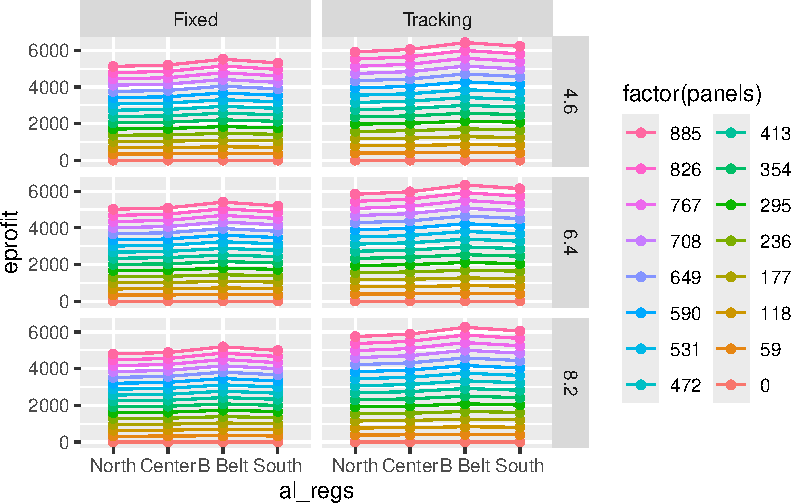
\includegraphics{Simulation_files/figure-pdf/unnamed-chunk-25-1.pdf}

\begin{verbatim}
Electricity Price =  0.015
\end{verbatim}

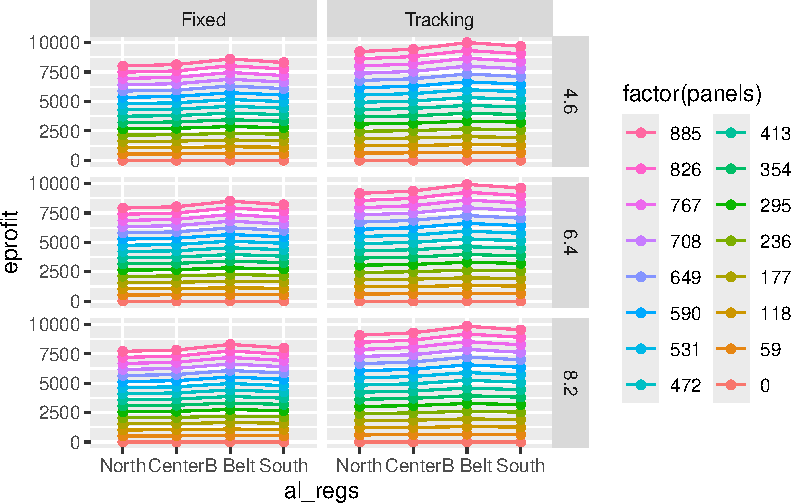
\includegraphics{Simulation_files/figure-pdf/unnamed-chunk-25-2.pdf}

\begin{verbatim}
Electricity Price =  0.02
\end{verbatim}

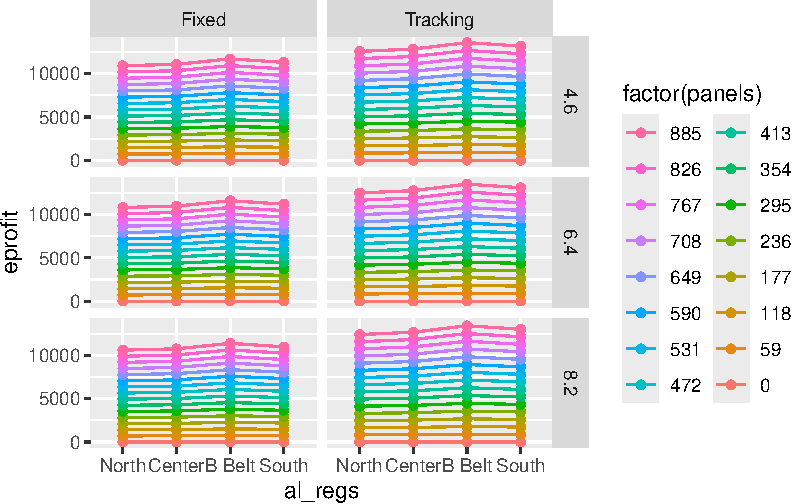
\includegraphics{Simulation_files/figure-pdf/unnamed-chunk-25-3.pdf}

\begin{verbatim}
Electricity Price =  0.025
\end{verbatim}

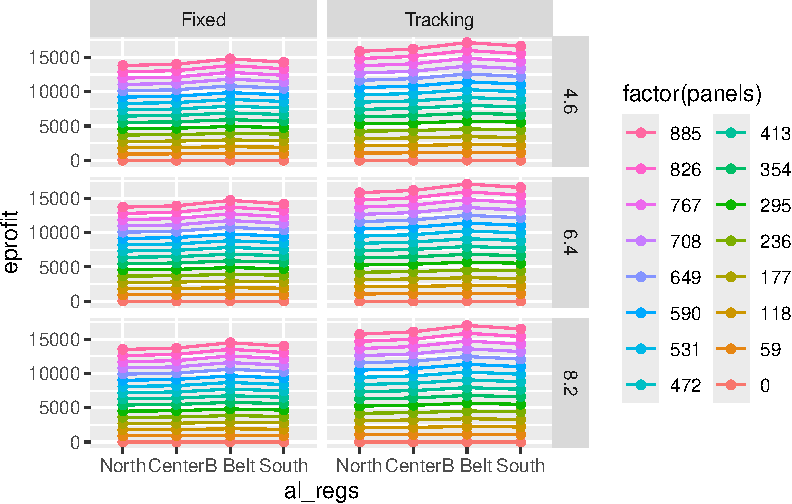
\includegraphics{Simulation_files/figure-pdf/unnamed-chunk-25-4.pdf}

\begin{verbatim}
Electricity Price =  0.03
\end{verbatim}

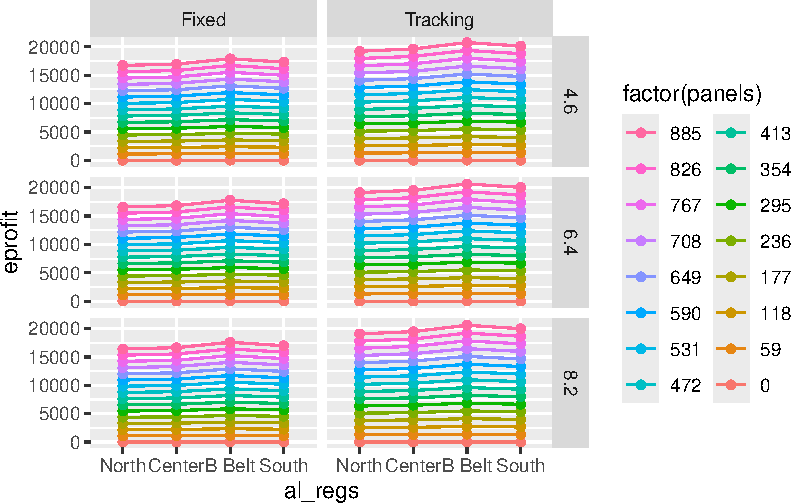
\includegraphics{Simulation_files/figure-pdf/unnamed-chunk-25-5.pdf}

\begin{verbatim}
Electricity Price =  0.035
\end{verbatim}

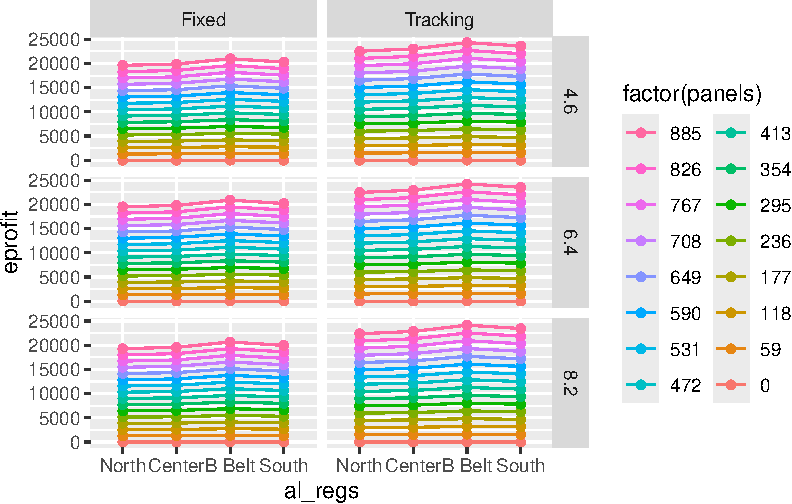
\includegraphics{Simulation_files/figure-pdf/unnamed-chunk-25-6.pdf}

\begin{verbatim}
Electricity Price =  0.04
\end{verbatim}

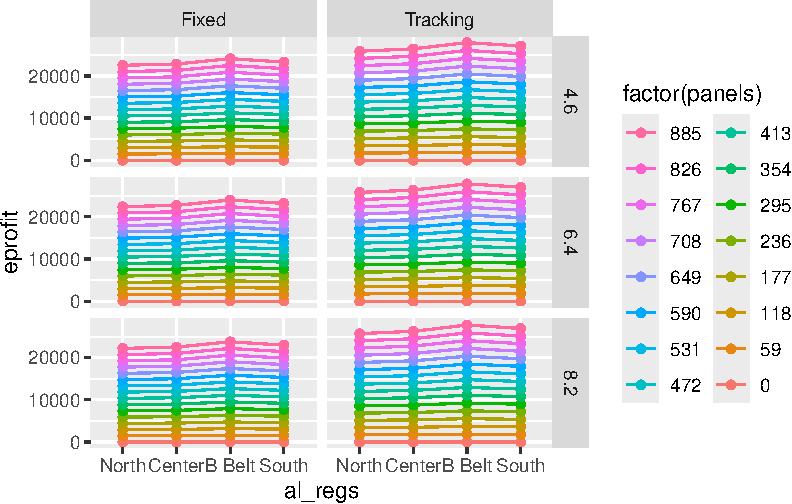
\includegraphics{Simulation_files/figure-pdf/unnamed-chunk-25-7.pdf}

\begin{verbatim}
Electricity Price =  0.045
\end{verbatim}

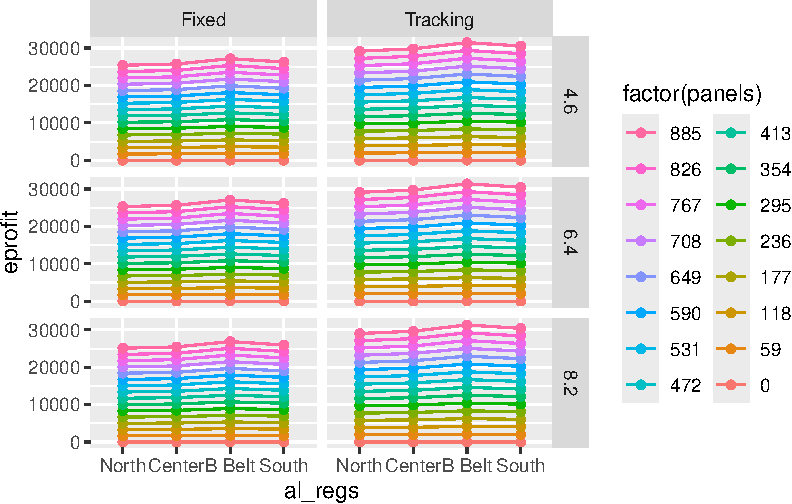
\includegraphics{Simulation_files/figure-pdf/unnamed-chunk-25-8.pdf}

\begin{verbatim}
Electricity Price =  0.05
\end{verbatim}

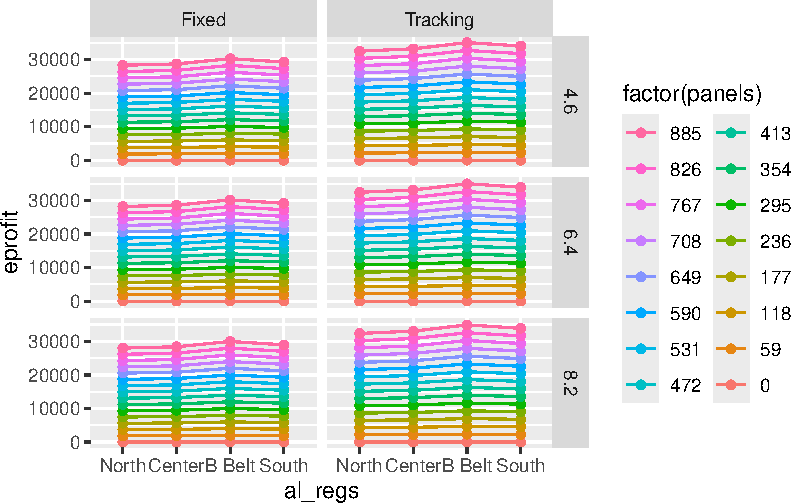
\includegraphics{Simulation_files/figure-pdf/unnamed-chunk-25-9.pdf}

\begin{verbatim}
Electricity Price =  0.055
\end{verbatim}

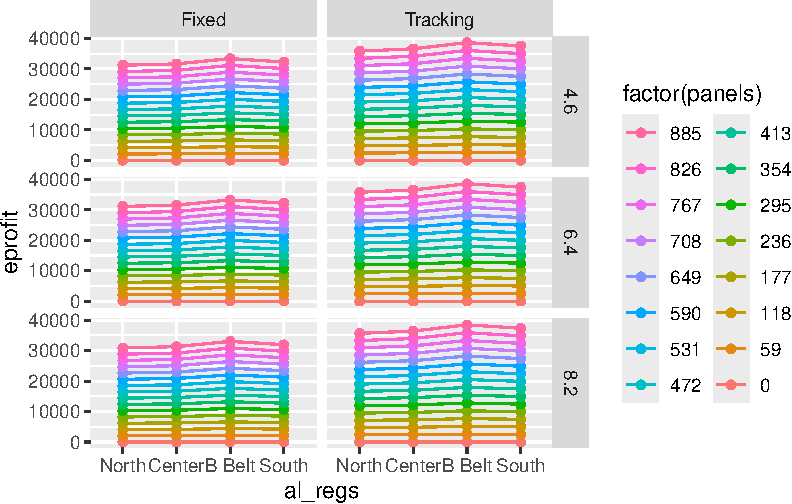
\includegraphics{Simulation_files/figure-pdf/unnamed-chunk-25-10.pdf}

\begin{verbatim}
Electricity Price =  0.06
\end{verbatim}

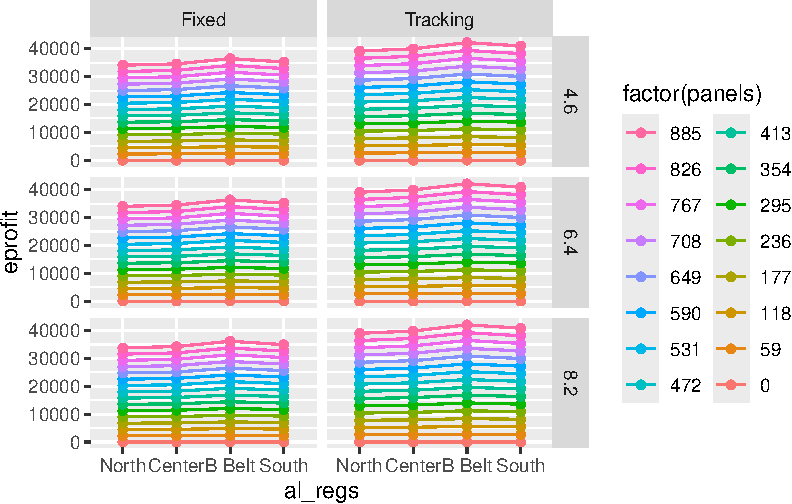
\includegraphics{Simulation_files/figure-pdf/unnamed-chunk-25-11.pdf}

\section{Profit from crops}\label{profit-from-crops}

\subsection{Tomato}\label{tomato-1}

Filter return to operator, land and capital profit from Tomato:

\begin{Shaded}
\begin{Highlighting}[]
\NormalTok{tomato\_profit }\OtherTok{=}\NormalTok{ tomato }\SpecialCharTok{\%\textgreater{}\%} 
  \FunctionTok{select}\NormalTok{(yldvar, yield, }
\NormalTok{         rolac17, rolac18, rolac19, rolac20, }
\NormalTok{         rolac21, rolac22, rolac23)}
\FunctionTok{dim}\NormalTok{(tomato\_profit)}
\end{Highlighting}
\end{Shaded}

\begin{verbatim}
[1] 20  9
\end{verbatim}

\begin{Shaded}
\begin{Highlighting}[]
\NormalTok{tomato\_profit}
\end{Highlighting}
\end{Shaded}

\begin{verbatim}
   yldvar yield    rolac17    rolac18    rolac19    rolac20    rolac21
3     2.0  2720 21679.3826 24399.3826 27119.3826 29839.3826 32559.3826
4     1.9  2584 20065.3826 22649.3826 25233.3826 27817.3826 30401.3826
5     1.8  2448 18451.3826 20899.3826 23347.3826 25795.3826 28243.3826
6     1.7  2312 16837.3826 19149.3826 21461.3826 23773.3826 26085.3826
7     1.6  2176 15223.3826 17399.3826 19575.3826 21751.3826 23927.3826
8     1.5  2040 13609.3826 15649.3826 17689.3826 19729.3826 21769.3826
9     1.4  1904 11995.3826 13899.3826 15803.3826 17707.3826 19611.3826
10    1.3  1768 10381.3826 12149.3826 13917.3826 15685.3826 17453.3826
11    1.2  1632  8767.3826 10399.3826 12031.3826 13663.3826 15295.3826
12    1.1  1496  7153.3826  8649.3826 10145.3826 11641.3826 13137.3826
13    1.0  1360  5539.3826  6899.3826  8259.3826  9619.3826 10979.3826
14    0.9  1224  3925.3826  5149.3826  6373.3826  7597.3826  8821.3826
15    0.8  1088  2311.3826  3399.3826  4487.3826  5575.3826  6663.3826
16    0.7   952   697.3826  1649.3826  2601.3826  3553.3826  4505.3826
17    0.6   816  -916.6174  -100.6174   715.3826  1531.3826  2347.3826
18    0.5   680 -2530.6174 -1850.6174 -1170.6174  -490.6174   189.3826
19    0.4   544 -4144.6174 -3600.6174 -3056.6174 -2512.6174 -1968.6174
20    0.3   408 -5758.6174 -5350.6174 -4942.6174 -4534.6174 -4126.6174
21    0.2   272 -7372.6174 -7100.6174 -6828.6174 -6556.6174 -6284.6174
22    0.1   136 -8986.6174 -8850.6174 -8714.6174 -8578.6174 -8442.6174
      rolac22    rolac23
3  35279.3826 37999.3826
4  32985.3826 35569.3826
5  30691.3826 33139.3826
6  28397.3826 30709.3826
7  26103.3826 28279.3826
8  23809.3826 25849.3826
9  21515.3826 23419.3826
10 19221.3826 20989.3826
11 16927.3826 18559.3826
12 14633.3826 16129.3826
13 12339.3826 13699.3826
14 10045.3826 11269.3826
15  7751.3826  8839.3826
16  5457.3826  6409.3826
17  3163.3826  3979.3826
18   869.3826  1549.3826
19 -1424.6174  -880.6174
20 -3718.6174 -3310.6174
21 -6012.6174 -5740.6174
22 -8306.6174 -8170.6174
\end{verbatim}

Convert data to long format:

\begin{Shaded}
\begin{Highlighting}[]
\CommentTok{\# Assign column names for clarity}
\FunctionTok{colnames}\NormalTok{(tomato\_profit) }\OtherTok{\textless{}{-}} \FunctionTok{c}\NormalTok{(}\StringTok{"yldvar"}\NormalTok{, }\StringTok{"yield"}\NormalTok{,}
                  \StringTok{"rolac17"}\NormalTok{, }\StringTok{"rolac18"}\NormalTok{, }\StringTok{"rolac19"}\NormalTok{,}
                  \StringTok{"rolac20"}\NormalTok{, }\StringTok{"rolac21"}\NormalTok{, }\StringTok{"rolac22"}\NormalTok{,}
                  \StringTok{"rolac23"}\NormalTok{)}

\CommentTok{\# Reshape the data frame from wide to long format}
\NormalTok{tomato\_long }\OtherTok{\textless{}{-}} \FunctionTok{melt}\NormalTok{(tomato\_profit,}
                \AttributeTok{id.vars =} \FunctionTok{c}\NormalTok{(}\StringTok{"yldvar"}\NormalTok{, }\StringTok{"yield"}\NormalTok{),}
                \AttributeTok{measure.vars =} \FunctionTok{c}\NormalTok{(}\StringTok{"rolac17"}\NormalTok{, }\StringTok{"rolac18"}\NormalTok{, }\StringTok{"rolac19"}\NormalTok{,}
                                 \StringTok{"rolac20"}\NormalTok{, }\StringTok{"rolac21"}\NormalTok{, }\StringTok{"rolac22"}\NormalTok{,}
                                 \StringTok{"rolac23"}\NormalTok{),}
                \AttributeTok{variable.name =} \StringTok{"price"}\NormalTok{,}
                \AttributeTok{value.name =} \StringTok{"profit"}\NormalTok{)}

\CommentTok{\# Convert the \textquotesingle{}Price\textquotesingle{} column to numeric by extracting the number}
\NormalTok{tomato\_long}\SpecialCharTok{$}\NormalTok{price }\OtherTok{\textless{}{-}} \FunctionTok{as.numeric}\NormalTok{(}\FunctionTok{gsub}\NormalTok{(}\StringTok{"rolac"}\NormalTok{, }\StringTok{""}\NormalTok{, tomato\_long}\SpecialCharTok{$}\NormalTok{price))}

\CommentTok{\# View the resulting data frame}
\FunctionTok{dim}\NormalTok{(tomato\_long)}
\end{Highlighting}
\end{Shaded}

\begin{verbatim}
[1] 140   4
\end{verbatim}

\begin{Shaded}
\begin{Highlighting}[]
\FunctionTok{head}\NormalTok{(tomato\_long)}
\end{Highlighting}
\end{Shaded}

\begin{verbatim}
  yldvar yield price   profit
1    2.0  2720    17 21679.38
2    1.9  2584    17 20065.38
3    1.8  2448    17 18451.38
4    1.7  2312    17 16837.38
5    1.6  2176    17 15223.38
6    1.5  2040    17 13609.38
\end{verbatim}

\begin{Shaded}
\begin{Highlighting}[]
\FunctionTok{tail}\NormalTok{(tomato\_long)}
\end{Highlighting}
\end{Shaded}

\begin{verbatim}
    yldvar yield price     profit
135    0.6   816    23  3979.3826
136    0.5   680    23  1549.3826
137    0.4   544    23  -880.6174
138    0.3   408    23 -3310.6174
139    0.2   272    23 -5740.6174
140    0.1   136    23 -8170.6174
\end{verbatim}

\subsubsection{Profit from tomato}\label{profit-from-tomato}

\begin{Shaded}
\begin{Highlighting}[]
\FunctionTok{ggplot}\NormalTok{(}\AttributeTok{data =}\NormalTok{ tomato\_long,}
       \AttributeTok{mapping =} \FunctionTok{aes}\NormalTok{(}\AttributeTok{x =}\NormalTok{ price,}
                     \AttributeTok{y =}\NormalTok{ profit,}
                     \AttributeTok{color =} \FunctionTok{factor}\NormalTok{(yldvar),}
                     \AttributeTok{group =} \FunctionTok{factor}\NormalTok{(yield))) }\SpecialCharTok{+}
  \FunctionTok{geom\_line}\NormalTok{() }\SpecialCharTok{+}
  \FunctionTok{geom\_point}\NormalTok{() }\SpecialCharTok{+}
  \FunctionTok{geom\_hline}\NormalTok{(}\AttributeTok{yintercept =} \DecValTok{0}\NormalTok{,}
             \AttributeTok{linetype =} \StringTok{"dashed"}\NormalTok{,}
             \AttributeTok{color =} \StringTok{"black"}\NormalTok{) }\SpecialCharTok{+}
  \FunctionTok{guides}\NormalTok{(}\AttributeTok{color =} \FunctionTok{guide\_legend}\NormalTok{(}\AttributeTok{ncol =} \DecValTok{2}\NormalTok{,}
                              \AttributeTok{reverse =} \ConstantTok{TRUE}\NormalTok{))}
\end{Highlighting}
\end{Shaded}

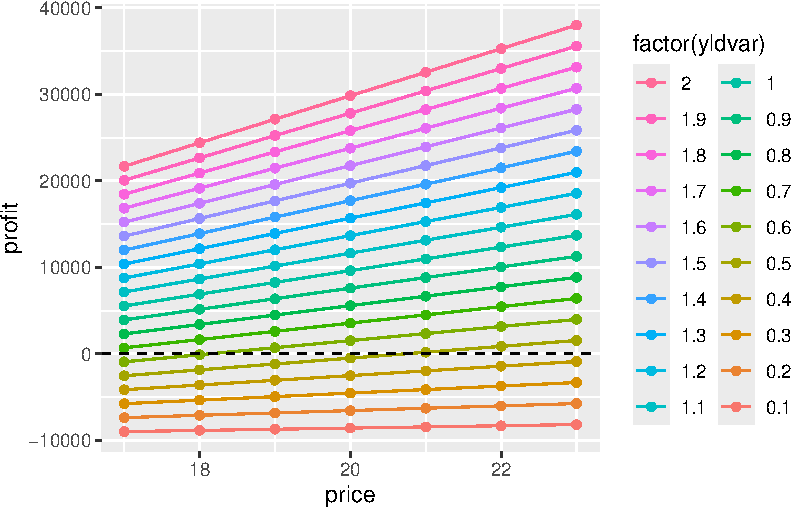
\includegraphics{Simulation_files/figure-pdf/unnamed-chunk-28-1.pdf}

\begin{Shaded}
\begin{Highlighting}[]
\FunctionTok{ggplot}\NormalTok{(}\AttributeTok{data =}\NormalTok{ tomato\_long,}
       \AttributeTok{mapping =} \FunctionTok{aes}\NormalTok{(}\AttributeTok{x =}\NormalTok{ yield,}
                     \AttributeTok{y =}\NormalTok{ profit,}
                     \CommentTok{\#fill = yield,}
                     \AttributeTok{color =} \FunctionTok{factor}\NormalTok{(price),}
                     \AttributeTok{group =} \FunctionTok{factor}\NormalTok{(price))) }\SpecialCharTok{+}
  \FunctionTok{geom\_line}\NormalTok{() }\SpecialCharTok{+}
  \FunctionTok{geom\_point}\NormalTok{() }\SpecialCharTok{+}
  \FunctionTok{geom\_hline}\NormalTok{(}\AttributeTok{yintercept =} \DecValTok{0}\NormalTok{,}
             \AttributeTok{linetype =} \StringTok{"dashed"}\NormalTok{,}
             \AttributeTok{color =} \StringTok{"black"}\NormalTok{) }\SpecialCharTok{+}
  \CommentTok{\# Vertical dashed line is 100\% yield}
  \FunctionTok{geom\_vline}\NormalTok{(}\AttributeTok{xintercept =}\NormalTok{ tomato\_long}\SpecialCharTok{$}\NormalTok{yield[}\DecValTok{11}\NormalTok{],}
             \AttributeTok{linetype =} \StringTok{"dashed"}\NormalTok{,}
             \AttributeTok{color =} \StringTok{"black"}\NormalTok{) }\SpecialCharTok{+}
\FunctionTok{guides}\NormalTok{(}\AttributeTok{color =} \FunctionTok{guide\_legend}\NormalTok{(}\AttributeTok{reverse =} \ConstantTok{TRUE}\NormalTok{))}
\end{Highlighting}
\end{Shaded}

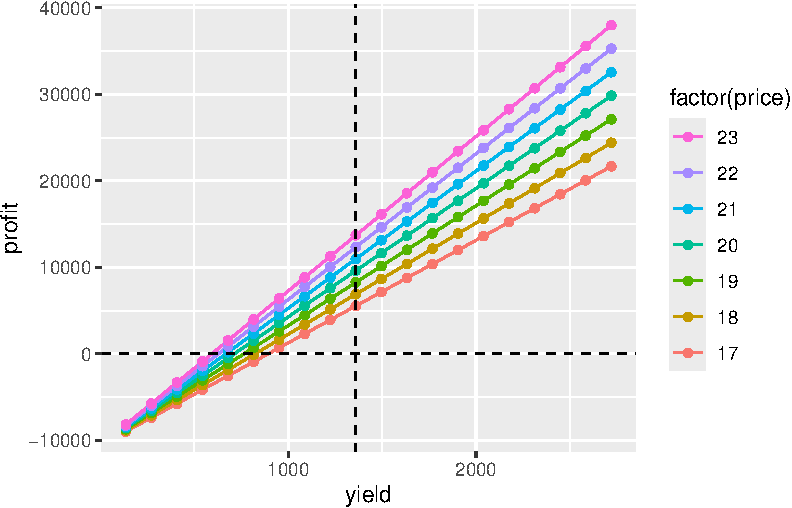
\includegraphics{Simulation_files/figure-pdf/unnamed-chunk-29-1.pdf}

\subsection{Strawberry}\label{strawberry-1}

Filter return to operator, land and capital profit from strawberry

\begin{Shaded}
\begin{Highlighting}[]
\NormalTok{strawberry\_profit }\OtherTok{=}\NormalTok{ strawberry }\SpecialCharTok{\%\textgreater{}\%} 
  \FunctionTok{select}\NormalTok{(yldvar, yield, }
\NormalTok{         rolac3, rolac4, rolac5, rolac6, }
\NormalTok{         rolac7, rolac8, rolac9)}
\FunctionTok{dim}\NormalTok{(strawberry\_profit)}
\end{Highlighting}
\end{Shaded}

\begin{verbatim}
[1] 20  9
\end{verbatim}

\begin{Shaded}
\begin{Highlighting}[]
\NormalTok{strawberry\_profit}
\end{Highlighting}
\end{Shaded}

\begin{verbatim}
   yldvar  yield     rolac3       rolac4     rolac5     rolac6     rolac7
3     2.0 6150.0  -1740.495   4409.50503  10559.505  16709.505  22859.505
4     1.9 5842.5  -2317.350   3525.15003   9367.650  15210.150  21052.650
5     1.8 5535.0  -2894.205   2640.79503   8175.795  13710.795  19245.795
6     1.7 5227.5  -3471.060   1756.44003   6983.940  12211.440  17438.940
7     1.6 4920.0  -4047.915    872.08503   5792.085  10712.085  15632.085
8     1.5 4612.5  -4624.770    -12.26997   4600.230   9212.730  13825.230
9     1.4 4305.0  -5201.625   -896.62497   3408.375   7713.375  12018.375
10    1.3 3997.5  -5778.480  -1780.97997   2216.520   6214.020  10211.520
11    1.2 3690.0  -6355.335  -2665.33497   1024.665   4714.665   8404.665
12    1.1 3382.5  -6932.190  -3549.68997   -167.190   3215.310   6597.810
13    1.0 3075.0  -7509.045  -4434.04497  -1359.045   1715.955   4790.955
14    0.9 2767.5  -8085.900  -5318.39997  -2550.900    216.600   2984.100
15    0.8 2460.0  -8662.755  -6202.75497  -3742.755  -1282.755   1177.245
16    0.7 2152.5  -9239.610  -7087.10997  -4934.610  -2782.110   -629.610
17    0.6 1845.0  -9816.465  -7971.46497  -6126.465  -4281.465  -2436.465
18    0.5 1537.5 -10393.320  -8855.81997  -7318.320  -5780.820  -4243.320
19    0.4 1230.0 -10970.175  -9740.17497  -8510.175  -7280.175  -6050.175
20    0.3  922.5 -11547.030 -10624.52997  -9702.030  -8779.530  -7857.030
21    0.2  615.0 -12123.885 -11508.88497 -10893.885 -10278.885  -9663.885
22    0.1  307.5 -12700.740 -12393.23997 -12085.740 -11778.240 -11470.740
       rolac8     rolac9
3   29009.505  35159.505
4   26895.150  32737.650
5   24780.795  30315.795
6   22666.440  27893.940
7   20552.085  25472.085
8   18437.730  23050.230
9   16323.375  20628.375
10  14209.020  18206.520
11  12094.665  15784.665
12   9980.310  13362.810
13   7865.955  10940.955
14   5751.600   8519.100
15   3637.245   6097.245
16   1522.890   3675.390
17   -591.465   1253.535
18  -2705.820  -1168.320
19  -4820.175  -3590.175
20  -6934.530  -6012.030
21  -9048.885  -8433.885
22 -11163.240 -10855.740
\end{verbatim}

Convert data to long format:

\begin{Shaded}
\begin{Highlighting}[]
\CommentTok{\# Assign column names for clarity}
\FunctionTok{colnames}\NormalTok{(strawberry\_profit) }\OtherTok{\textless{}{-}} \FunctionTok{c}\NormalTok{(}\StringTok{"yldvar"}\NormalTok{, }\StringTok{"yield"}\NormalTok{,}
                  \StringTok{"rolac3"}\NormalTok{, }\StringTok{"rolac4"}\NormalTok{, }\StringTok{"rolac5"}\NormalTok{,}
                  \StringTok{"rolac6"}\NormalTok{, }\StringTok{"rolac7"}\NormalTok{, }\StringTok{"rolac8"}\NormalTok{,}
                  \StringTok{"rolac9"}\NormalTok{)}
\CommentTok{\# Reshape the data frame from wide to long format}
\NormalTok{stberry\_long }\OtherTok{\textless{}{-}} \FunctionTok{melt}\NormalTok{(strawberry\_profit,}
                \AttributeTok{id.vars =} \FunctionTok{c}\NormalTok{(}\StringTok{"yldvar"}\NormalTok{, }\StringTok{"yield"}\NormalTok{),}
                \AttributeTok{measure.vars =} \FunctionTok{c}\NormalTok{(}\StringTok{"rolac3"}\NormalTok{, }\StringTok{"rolac4"}\NormalTok{, }\StringTok{"rolac5"}\NormalTok{,}
                                 \StringTok{"rolac6"}\NormalTok{, }\StringTok{"rolac7"}\NormalTok{, }\StringTok{"rolac8"}\NormalTok{,}
                                 \StringTok{"rolac9"}\NormalTok{),}
                \AttributeTok{variable.name =} \StringTok{"price"}\NormalTok{,}
                \AttributeTok{value.name =} \StringTok{"profit"}\NormalTok{)}

\CommentTok{\# Convert the \textquotesingle{}Price\textquotesingle{} column to numeric by extracting the number}
\NormalTok{stberry\_long}\SpecialCharTok{$}\NormalTok{price }\OtherTok{\textless{}{-}} \FunctionTok{as.numeric}\NormalTok{(}\FunctionTok{gsub}\NormalTok{(}\StringTok{"rolac"}\NormalTok{, }\StringTok{""}\NormalTok{, stberry\_long}\SpecialCharTok{$}\NormalTok{price))}

\CommentTok{\# View the resulting data frame}
\FunctionTok{dim}\NormalTok{(stberry\_long)}
\end{Highlighting}
\end{Shaded}

\begin{verbatim}
[1] 140   4
\end{verbatim}

\begin{Shaded}
\begin{Highlighting}[]
\FunctionTok{head}\NormalTok{(stberry\_long)}
\end{Highlighting}
\end{Shaded}

\begin{verbatim}
  yldvar  yield price    profit
1    2.0 6150.0     3 -1740.495
2    1.9 5842.5     3 -2317.350
3    1.8 5535.0     3 -2894.205
4    1.7 5227.5     3 -3471.060
5    1.6 4920.0     3 -4047.915
6    1.5 4612.5     3 -4624.770
\end{verbatim}

\begin{Shaded}
\begin{Highlighting}[]
\FunctionTok{tail}\NormalTok{(stberry\_long)}
\end{Highlighting}
\end{Shaded}

\begin{verbatim}
    yldvar  yield price     profit
135    0.6 1845.0     9   1253.535
136    0.5 1537.5     9  -1168.320
137    0.4 1230.0     9  -3590.175
138    0.3  922.5     9  -6012.030
139    0.2  615.0     9  -8433.885
140    0.1  307.5     9 -10855.740
\end{verbatim}

\subsubsection{Plot Strawberry Profit}\label{plot-strawberry-profit}

\begin{Shaded}
\begin{Highlighting}[]
\FunctionTok{ggplot}\NormalTok{(}\AttributeTok{data =}\NormalTok{ stberry\_long,}
       \AttributeTok{mapping =} \FunctionTok{aes}\NormalTok{(}\AttributeTok{x =}\NormalTok{ price,}
                     \AttributeTok{y =}\NormalTok{ profit,}
                     \AttributeTok{color =} \FunctionTok{factor}\NormalTok{(yldvar),}
                     \AttributeTok{group =} \FunctionTok{factor}\NormalTok{(yield))) }\SpecialCharTok{+}
  \FunctionTok{geom\_line}\NormalTok{() }\SpecialCharTok{+}
  \FunctionTok{geom\_point}\NormalTok{() }\SpecialCharTok{+}
  \FunctionTok{geom\_hline}\NormalTok{(}\AttributeTok{yintercept =} \DecValTok{0}\NormalTok{,}
             \AttributeTok{linetype =} \StringTok{"dashed"}\NormalTok{,}
             \AttributeTok{color =} \StringTok{"black"}\NormalTok{) }\SpecialCharTok{+}
  \FunctionTok{guides}\NormalTok{(}\AttributeTok{color =} \FunctionTok{guide\_legend}\NormalTok{(}\AttributeTok{ncol =} \DecValTok{2}\NormalTok{,}
                              \AttributeTok{reverse =} \ConstantTok{TRUE}\NormalTok{))}
\end{Highlighting}
\end{Shaded}

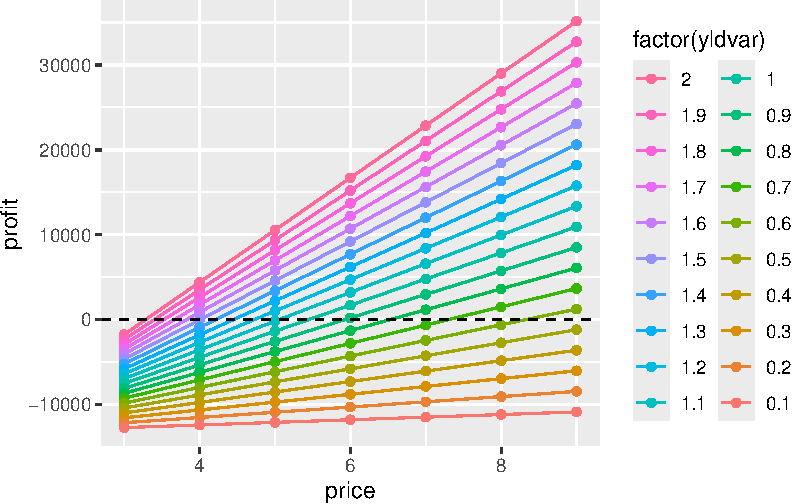
\includegraphics{Simulation_files/figure-pdf/unnamed-chunk-32-1.pdf}

\begin{Shaded}
\begin{Highlighting}[]
\FunctionTok{ggplot}\NormalTok{(}\AttributeTok{data =}\NormalTok{ stberry\_long,}
       \AttributeTok{mapping =} \FunctionTok{aes}\NormalTok{(}\AttributeTok{x =}\NormalTok{ yield,}
                     \AttributeTok{y =}\NormalTok{ profit,}
                     \AttributeTok{color =} \FunctionTok{factor}\NormalTok{(price),}
                     \AttributeTok{group =} \FunctionTok{factor}\NormalTok{(price))) }\SpecialCharTok{+}
  \FunctionTok{geom\_line}\NormalTok{() }\SpecialCharTok{+}
  \FunctionTok{geom\_point}\NormalTok{() }\SpecialCharTok{+}
  \FunctionTok{geom\_hline}\NormalTok{(}\AttributeTok{yintercept =} \DecValTok{0}\NormalTok{,}
             \AttributeTok{linetype =} \StringTok{"dashed"}\NormalTok{,}
             \AttributeTok{color =} \StringTok{"black"}\NormalTok{) }\SpecialCharTok{+}
  \CommentTok{\#Vertical dashed line is 100\% yield}
  \FunctionTok{geom\_vline}\NormalTok{(}\AttributeTok{xintercept =}\NormalTok{ stberry\_long}\SpecialCharTok{$}\NormalTok{yield[}\DecValTok{11}\NormalTok{],}
             \AttributeTok{linetype =} \StringTok{"dashed"}\NormalTok{,}
             \AttributeTok{color =} \StringTok{"black"}\NormalTok{) }\SpecialCharTok{+}
  \FunctionTok{guides}\NormalTok{(}\AttributeTok{color =} \FunctionTok{guide\_legend}\NormalTok{(}\AttributeTok{reverse =} \ConstantTok{TRUE}\NormalTok{))}
\end{Highlighting}
\end{Shaded}

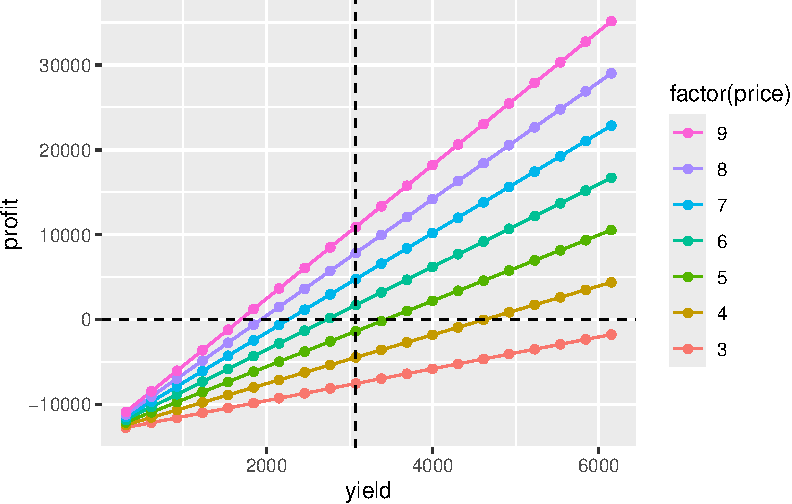
\includegraphics{Simulation_files/figure-pdf/unnamed-chunk-33-1.pdf}

\subsection{Squash}\label{squash-1}

Filter return to operator, land and capital profit from squash

\begin{Shaded}
\begin{Highlighting}[]
\NormalTok{squash\_profit }\OtherTok{=}\NormalTok{ squash }\SpecialCharTok{\%\textgreater{}\%} 
  \FunctionTok{select}\NormalTok{(yldvar, yield, }
\NormalTok{         rolac11, rolac12, rolac13, rolac14, }
\NormalTok{         rolac15, rolac16, rolac17)}
\NormalTok{squash\_profit}
\end{Highlighting}
\end{Shaded}

\begin{verbatim}
   yldvar yield   rolac11   rolac12     rolac13   rolac14   rolac15     rolac16
3     2.0  2180 10309.117 12489.117 14669.11702 16849.117 19029.117 21209.11702
4     1.9  2071  9607.367 11678.367 13749.36702 15820.367 17891.367 19962.36702
5     1.8  1962  8905.617 10867.617 12829.61702 14791.617 16753.617 18715.61702
6     1.7  1853  8203.867 10056.867 11909.86702 13762.867 15615.867 17468.86702
7     1.6  1744  7502.117  9246.117 10990.11702 12734.117 14478.117 16222.11702
8     1.5  1635  6800.367  8435.367 10070.36702 11705.367 13340.367 14975.36702
9     1.4  1526  6098.617  7624.617  9150.61702 10676.617 12202.617 13728.61702
10    1.3  1417  5396.867  6813.867  8230.86702  9647.867 11064.867 12481.86702
11    1.2  1308  4695.117  6003.117  7311.11702  8619.117  9927.117 11235.11702
12    1.1  1199  3993.367  5192.367  6391.36702  7590.367  8789.367  9988.36702
13    1.0  1090  3291.617  4381.617  5471.61702  6561.617  7651.617  8741.61702
14    0.9   981  2589.867  3570.867  4551.86702  5532.867  6513.867  7494.86702
15    0.8   872  1888.117  2760.117  3632.11702  4504.117  5376.117  6248.11702
16    0.7   763  1186.367  1949.367  2712.36702  3475.367  4238.367  5001.36702
17    0.6   654   484.617  1138.617  1792.61702  2446.617  3100.617  3754.61702
18    0.5   545  -217.133   327.867   872.86702  1417.867  1962.867  2507.86702
19    0.4   436  -918.883  -482.883   -46.88298   389.117   825.117  1261.11702
20    0.3   327 -1620.633 -1293.633  -966.63298  -639.633  -312.633    14.36702
21    0.2   218 -2322.383 -2104.383 -1886.38298 -1668.383 -1450.383 -1232.38298
22    0.1   109 -3024.133 -2915.133 -2806.13298 -2697.133 -2588.133 -2479.13298
     rolac17
3  23389.117
4  22033.367
5  20677.617
6  19321.867
7  17966.117
8  16610.367
9  15254.617
10 13898.867
11 12543.117
12 11187.367
13  9831.617
14  8475.867
15  7120.117
16  5764.367
17  4408.617
18  3052.867
19  1697.117
20   341.367
21 -1014.383
22 -2370.133
\end{verbatim}

Convert data to long format:

\begin{Shaded}
\begin{Highlighting}[]
\CommentTok{\# Assign column names for clarity}
\FunctionTok{colnames}\NormalTok{(squash\_profit) }\OtherTok{\textless{}{-}} \FunctionTok{c}\NormalTok{(}\StringTok{"yldvar"}\NormalTok{, }\StringTok{"yield"}\NormalTok{,}
                  \StringTok{"rolac11"}\NormalTok{, }\StringTok{"rolac12"}\NormalTok{, }\StringTok{"rolac13"}\NormalTok{,}
                  \StringTok{"rolac14"}\NormalTok{, }\StringTok{"rolac15"}\NormalTok{, }\StringTok{"rolac16"}\NormalTok{,}
                  \StringTok{"rolac17"}\NormalTok{)}

\CommentTok{\# Reshape the data frame from wide to long format}
\NormalTok{squash\_long }\OtherTok{\textless{}{-}} \FunctionTok{melt}\NormalTok{(squash\_profit,}
                \AttributeTok{id.vars =} \FunctionTok{c}\NormalTok{(}\StringTok{"yldvar"}\NormalTok{, }\StringTok{"yield"}\NormalTok{),}
                \AttributeTok{measure.vars =} \FunctionTok{c}\NormalTok{(}\StringTok{"rolac11"}\NormalTok{, }\StringTok{"rolac12"}\NormalTok{, }\StringTok{"rolac13"}\NormalTok{,}
                                 \StringTok{"rolac14"}\NormalTok{, }\StringTok{"rolac15"}\NormalTok{, }\StringTok{"rolac16"}\NormalTok{,}
                                 \StringTok{"rolac17"}\NormalTok{),}
                \AttributeTok{variable.name =} \StringTok{"price"}\NormalTok{,}
                \AttributeTok{value.name =} \StringTok{"profit"}\NormalTok{)}

\CommentTok{\# Convert the \textquotesingle{}Price\textquotesingle{} column to numeric by extracting the number}
\NormalTok{squash\_long}\SpecialCharTok{$}\NormalTok{price }\OtherTok{\textless{}{-}} \FunctionTok{as.numeric}\NormalTok{(}\FunctionTok{gsub}\NormalTok{(}\StringTok{"rolac"}\NormalTok{, }\StringTok{""}\NormalTok{, squash\_long}\SpecialCharTok{$}\NormalTok{price))}

\CommentTok{\# View the resulting data frame}
\FunctionTok{dim}\NormalTok{(squash\_long)}
\end{Highlighting}
\end{Shaded}

\begin{verbatim}
[1] 140   4
\end{verbatim}

\begin{Shaded}
\begin{Highlighting}[]
\FunctionTok{head}\NormalTok{(squash\_long)}
\end{Highlighting}
\end{Shaded}

\begin{verbatim}
  yldvar yield price    profit
1    2.0  2180    11 10309.117
2    1.9  2071    11  9607.367
3    1.8  1962    11  8905.617
4    1.7  1853    11  8203.867
5    1.6  1744    11  7502.117
6    1.5  1635    11  6800.367
\end{verbatim}

\begin{Shaded}
\begin{Highlighting}[]
\FunctionTok{tail}\NormalTok{(squash\_long)}
\end{Highlighting}
\end{Shaded}

\begin{verbatim}
    yldvar yield price    profit
135    0.6   654    17  4408.617
136    0.5   545    17  3052.867
137    0.4   436    17  1697.117
138    0.3   327    17   341.367
139    0.2   218    17 -1014.383
140    0.1   109    17 -2370.133
\end{verbatim}

\subsubsection{Profit from squash:}\label{profit-from-squash}

\begin{Shaded}
\begin{Highlighting}[]
\FunctionTok{ggplot}\NormalTok{(}\AttributeTok{data =}\NormalTok{ squash\_long,}
       \AttributeTok{mapping =} \FunctionTok{aes}\NormalTok{(}\AttributeTok{x =}\NormalTok{ price,}
                     \AttributeTok{y =}\NormalTok{ profit,}
                     \AttributeTok{color =} \FunctionTok{factor}\NormalTok{(yldvar),}
                     \AttributeTok{group =} \FunctionTok{factor}\NormalTok{(yield))) }\SpecialCharTok{+}
  \FunctionTok{geom\_line}\NormalTok{() }\SpecialCharTok{+}
  \FunctionTok{geom\_point}\NormalTok{() }\SpecialCharTok{+}
  \FunctionTok{geom\_hline}\NormalTok{(}\AttributeTok{yintercept =} \DecValTok{0}\NormalTok{,}
             \AttributeTok{linetype =} \StringTok{"dashed"}\NormalTok{,}
             \AttributeTok{color =} \StringTok{"black"}\NormalTok{) }\SpecialCharTok{+}
  \FunctionTok{guides}\NormalTok{(}\AttributeTok{color =} \FunctionTok{guide\_legend}\NormalTok{(}\AttributeTok{ncol =} \DecValTok{2}\NormalTok{, }
                              \AttributeTok{reverse =} \ConstantTok{TRUE}\NormalTok{))}
\end{Highlighting}
\end{Shaded}

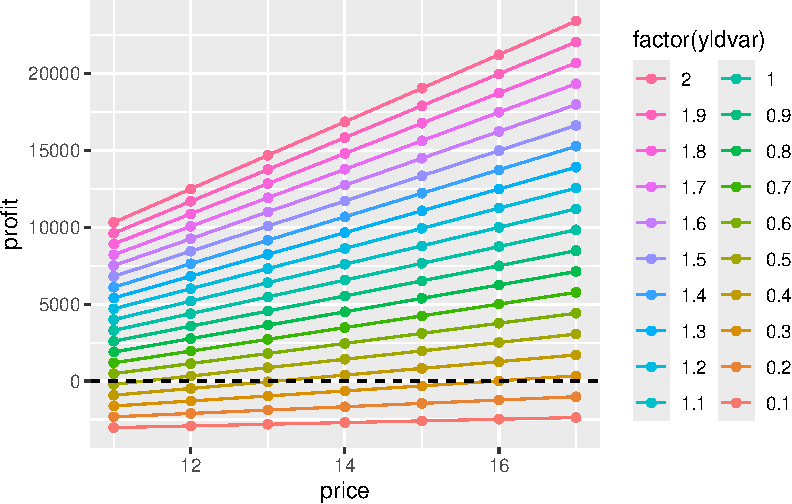
\includegraphics{Simulation_files/figure-pdf/unnamed-chunk-36-1.pdf}

\begin{Shaded}
\begin{Highlighting}[]
\FunctionTok{ggplot}\NormalTok{(}\AttributeTok{data =}\NormalTok{ squash\_long,}
       \AttributeTok{mapping =} \FunctionTok{aes}\NormalTok{(}\AttributeTok{x =}\NormalTok{ yield,}
                     \AttributeTok{y =}\NormalTok{ profit,}
                     \AttributeTok{color =} \FunctionTok{factor}\NormalTok{(price),}
                     \AttributeTok{group =} \FunctionTok{factor}\NormalTok{(price))) }\SpecialCharTok{+}
  \FunctionTok{geom\_line}\NormalTok{() }\SpecialCharTok{+}
  \FunctionTok{geom\_point}\NormalTok{() }\SpecialCharTok{+}
  \FunctionTok{geom\_hline}\NormalTok{(}\AttributeTok{yintercept =} \DecValTok{0}\NormalTok{,}
             \AttributeTok{linetype =} \StringTok{"dashed"}\NormalTok{,}
             \AttributeTok{color =} \StringTok{"black"}\NormalTok{) }\SpecialCharTok{+}
  \CommentTok{\# Vertical dashed line is 100\% yield}
    \FunctionTok{geom\_vline}\NormalTok{(}\AttributeTok{xintercept =}\NormalTok{ squash\_long}\SpecialCharTok{$}\NormalTok{yield[}\DecValTok{11}\NormalTok{],}
             \AttributeTok{linetype =} \StringTok{"dashed"}\NormalTok{,}
             \AttributeTok{color =} \StringTok{"black"}\NormalTok{) }\SpecialCharTok{+}
  \FunctionTok{guides}\NormalTok{(}\AttributeTok{color =} \FunctionTok{guide\_legend}\NormalTok{(}\AttributeTok{reverse =} \ConstantTok{TRUE}\NormalTok{))}
\end{Highlighting}
\end{Shaded}

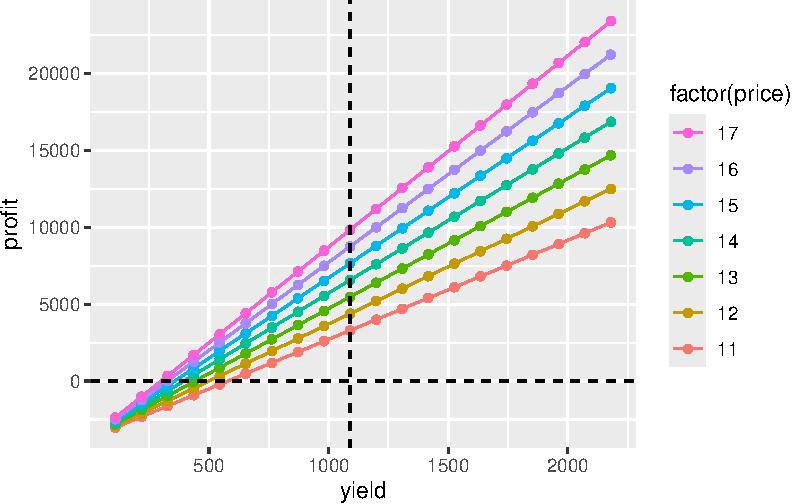
\includegraphics{Simulation_files/figure-pdf/unnamed-chunk-37-1.pdf}

\section{Profit from agrivoltaics}\label{profit-from-agrivoltaics}

Total profit from solar and crops for all combinations of AVs simulated.

\subsection{Profit from tomato agrivoltaic
system}\label{profit-from-tomato-agrivoltaic-system}

\begin{itemize}
\tightlist
\item
  Joint profit from tomato (tomato\_long) and solar energy production
  (solar\_profit) from 1 acre of land.
\item
  The last variable (tav\_profit) is the final profit from tomato
  agrivoltaic system which is the result of our interest.
\end{itemize}

\begin{Shaded}
\begin{Highlighting}[]
\CommentTok{\# Generate all combinations of row indices from both matrices}
\NormalTok{index\_combinations }\OtherTok{\textless{}{-}} \FunctionTok{expand.grid}\NormalTok{(}\DecValTok{1}\SpecialCharTok{:}\FunctionTok{nrow}\NormalTok{(solar\_profit),}
                                  \DecValTok{1}\SpecialCharTok{:}\FunctionTok{nrow}\NormalTok{(tomato\_long))}

\CommentTok{\# Define a function to process each combination of indices}
\NormalTok{process\_combination }\OtherTok{\textless{}{-}} \ControlFlowTok{function}\NormalTok{(indices) \{}
\NormalTok{  i }\OtherTok{\textless{}{-}}\NormalTok{ indices[}\DecValTok{1}\NormalTok{]}
\NormalTok{  j }\OtherTok{\textless{}{-}}\NormalTok{ indices[}\DecValTok{2}\NormalTok{]}
\NormalTok{  new\_row }\OtherTok{\textless{}{-}} \FunctionTok{c}\NormalTok{(solar\_profit[i, ],}
\NormalTok{               tomato\_long[j, ], }
               \CommentTok{\#solar\_profit[i, 14] = eannprof}
\NormalTok{               solar\_profit}\SpecialCharTok{$}\NormalTok{eannprof[i] }\SpecialCharTok{+}\NormalTok{ tomato\_long}\SpecialCharTok{$}\NormalTok{profit[j]) }
  \FunctionTok{return}\NormalTok{(new\_row)}
\NormalTok{\}}

\CommentTok{\# Apply the function to each combination of indices}
\CommentTok{\# Combine the results into a matrix}
\NormalTok{tav\_profit }\OtherTok{\textless{}{-}} \FunctionTok{do.call}\NormalTok{(rbind,}
                          \FunctionTok{lapply}\NormalTok{(}
                            \FunctionTok{seq\_len}\NormalTok{(}\FunctionTok{nrow}\NormalTok{(index\_combinations)),}
                            \ControlFlowTok{function}\NormalTok{(k) \{}
\NormalTok{                              indices }\OtherTok{\textless{}{-}} \FunctionTok{as.integer}\NormalTok{(}
\NormalTok{                                index\_combinations[k, ])}
                              \FunctionTok{process\_combination}\NormalTok{(indices)}
\NormalTok{                              \}))}

\CommentTok{\# Optionally, you can convert the result back to a data frame if needed}
\NormalTok{tav\_profit }\OtherTok{\textless{}{-}} \FunctionTok{as.data.frame}\NormalTok{(tav\_profit) }\SpecialCharTok{\%\textgreater{}\%}
    \FunctionTok{rename}\NormalTok{(}\AttributeTok{tav\_profit =}\NormalTok{ V21)}
\NormalTok{tav\_profit }\OtherTok{\textless{}{-}} \FunctionTok{data.frame}\NormalTok{(}\FunctionTok{lapply}\NormalTok{(tav\_profit, unlist))}
\FunctionTok{str}\NormalTok{(tav\_profit)}
\end{Highlighting}
\end{Shaded}

\begin{verbatim}
'data.frame':   776160 obs. of  21 variables:
 $ sprop     : num  0 0 0 0 0 0 0 0 0 0 ...
 $ al_regs   : chr  "Black Belt" "Black Belt" "Black Belt" "Black Belt" ...
 $ array     : chr  "Fixed" "Fixed" "Fixed" "Tracking" ...
 $ dc_kw     : num  0 0 0 0 0 0 0 0 0 0 ...
 $ panels    : num  0 0 0 0 0 0 0 0 0 0 ...
 $ energy    : num  0 0 0 0 0 0 0 0 0 0 ...
 $ elcprc    : num  0.01 0.01 0.01 0.01 0.01 0.01 0.01 0.01 0.01 0.01 ...
 $ elcrev    : num  0 0 0 0 0 0 0 0 0 0 ...
 $ height    : num  4.6 6.4 8.2 4.6 6.4 8.2 4.6 6.4 8.2 4.6 ...
 $ capex     : num  1.59 1.85 2.33 1.73 1.92 ...
 $ ttlcost   : num  0 0 0 0 0 0 0 0 0 0 ...
 $ anncost   : num  0 0 0 0 0 0 0 0 0 0 ...
 $ moncost   : num  0 0 0 0 0 0 0 0 0 0 ...
 $ eprofit   : num  0 0 0 0 0 0 0 0 0 0 ...
 $ eannprof  : num  0 0 0 0 0 0 0 0 0 0 ...
 $ emonprof  : num  0 0 0 0 0 0 0 0 0 0 ...
 $ yldvar    : num  2 2 2 2 2 2 2 2 2 2 ...
 $ yield     : num  2720 2720 2720 2720 2720 2720 2720 2720 2720 2720 ...
 $ price     : num  17 17 17 17 17 17 17 17 17 17 ...
 $ profit    : num  21679 21679 21679 21679 21679 ...
 $ tav_profit: num  21679 21679 21679 21679 21679 ...
\end{verbatim}

\begin{Shaded}
\begin{Highlighting}[]
\FunctionTok{head}\NormalTok{(tav\_profit)}
\end{Highlighting}
\end{Shaded}

\begin{verbatim}
  sprop    al_regs    array dc_kw panels energy elcprc elcrev height    capex
1     0 Black Belt    Fixed     0      0      0   0.01      0    4.6 1.593333
2     0 Black Belt    Fixed     0      0      0   0.01      0    6.4 1.850000
3     0 Black Belt    Fixed     0      0      0   0.01      0    8.2 2.330000
4     0 Black Belt Tracking     0      0      0   0.01      0    4.6 1.733333
5     0 Black Belt Tracking     0      0      0   0.01      0    6.4 1.921667
6     0 Black Belt Tracking     0      0      0   0.01      0    8.2 2.110000
  ttlcost anncost moncost eprofit eannprof emonprof yldvar yield price   profit
1       0       0       0       0        0        0      2  2720    17 21679.38
2       0       0       0       0        0        0      2  2720    17 21679.38
3       0       0       0       0        0        0      2  2720    17 21679.38
4       0       0       0       0        0        0      2  2720    17 21679.38
5       0       0       0       0        0        0      2  2720    17 21679.38
6       0       0       0       0        0        0      2  2720    17 21679.38
  tav_profit
1   21679.38
2   21679.38
3   21679.38
4   21679.38
5   21679.38
6   21679.38
\end{verbatim}

\begin{Shaded}
\begin{Highlighting}[]
\FunctionTok{tail}\NormalTok{(tav\_profit)}
\end{Highlighting}
\end{Shaded}

\begin{verbatim}
       sprop  al_regs    array  dc_kw panels   energy elcprc   elcrev height
776155     1 Southern    Fixed 423.74    885 598720.5   0.06 35923.23    4.6
776156     1 Southern    Fixed 423.74    885 598720.5   0.06 35923.23    6.4
776157     1 Southern    Fixed 423.74    885 598720.5   0.06 35923.23    8.2
776158     1 Southern Tracking 423.74    885 695415.0   0.06 41724.90    4.6
776159     1 Southern Tracking 423.74    885 695415.0   0.06 41724.90    6.4
776160     1 Southern Tracking 423.74    885 695415.0   0.06 41724.90    8.2
          capex  ttlcost  anncost  moncost  eprofit eannprof emonprof yldvar
776155 1.593333 675.1591 47.90419 3.946913 35248.07 35875.33 2989.656    0.1
776156 1.850000 783.9190 55.62098 4.582712 35139.31 35867.61 2989.020    0.1
776157 2.330000 987.3142 70.05237 5.771740 34935.92 35853.18 2987.831    0.1
776158 1.733333 734.4827 52.11335 4.293713 40990.42 41672.79 3472.781    0.1
776159 1.921667 814.2870 57.77567 4.760241 40910.61 41667.12 3472.315    0.1
776160 2.110000 894.0914 63.43798 5.226769 40830.81 41661.46 3471.848    0.1
       yield price    profit tav_profit
776155   136    23 -8170.617   27704.71
776156   136    23 -8170.617   27696.99
776157   136    23 -8170.617   27682.56
776158   136    23 -8170.617   33502.17
776159   136    23 -8170.617   33496.51
776160   136    23 -8170.617   33490.84
\end{verbatim}

\subsubsection{Saving results locally}\label{saving-results-locally}

\begin{Shaded}
\begin{Highlighting}[]
\CommentTok{\#write\_csv(tav\_profit, "tav\_profit.csv")}
\FunctionTok{write\_feather}\NormalTok{(tav\_profit,}
  \AttributeTok{sink =} \StringTok{"tav\_profit.feather"}\NormalTok{,}
  \AttributeTok{version =} \DecValTok{2}\NormalTok{,}
  \AttributeTok{chunk\_size =} \DecValTok{65536}\NormalTok{L,}
  \AttributeTok{compression =} \FunctionTok{c}\NormalTok{(}\StringTok{"default"}\NormalTok{),}
  \CommentTok{\#compression = c("default", "lz4", "lz4\_frame", "uncompressed", "zstd"),}
  \AttributeTok{compression\_level =} \ConstantTok{NULL}
\NormalTok{)}
\end{Highlighting}
\end{Shaded}

\subsection{Profit from strawberry agrivoltaic
system}\label{profit-from-strawberry-agrivoltaic-system}

\begin{itemize}
\tightlist
\item
  Joint profit from strawberry (stberry\_long) and solar energy
  production (solar\_profit) from 1 acre of land.
\item
  The last variable (sbav\_profit) is the final profit from strawberry
  agrivoltaic system which is the result of our interest.
\end{itemize}

\begin{Shaded}
\begin{Highlighting}[]
\CommentTok{\# Generate all combinations of row indices from both matrices}
\NormalTok{index\_combinations }\OtherTok{\textless{}{-}} \FunctionTok{expand.grid}\NormalTok{(}\DecValTok{1}\SpecialCharTok{:}\FunctionTok{nrow}\NormalTok{(solar\_profit),}
                                  \DecValTok{1}\SpecialCharTok{:}\FunctionTok{nrow}\NormalTok{(stberry\_long))}

\CommentTok{\# Define a function to process each combination of indices}
\NormalTok{process\_combination }\OtherTok{\textless{}{-}} \ControlFlowTok{function}\NormalTok{(indices) \{}
\NormalTok{  i }\OtherTok{\textless{}{-}}\NormalTok{ indices[}\DecValTok{1}\NormalTok{]}
\NormalTok{  j }\OtherTok{\textless{}{-}}\NormalTok{ indices[}\DecValTok{2}\NormalTok{]}
\NormalTok{  new\_row }\OtherTok{\textless{}{-}} \FunctionTok{c}\NormalTok{(solar\_profit[i, ],}
\NormalTok{               stberry\_long[j, ], }
               \CommentTok{\#solar\_profit[i, 14] = eannprof}
\NormalTok{               solar\_profit}\SpecialCharTok{$}\NormalTok{eannprof[i] }\SpecialCharTok{+}\NormalTok{ stberry\_long}\SpecialCharTok{$}\NormalTok{profit[j])}
  \FunctionTok{return}\NormalTok{(new\_row)}
\NormalTok{\}}

\CommentTok{\# Apply the function to each combination of indices}
\CommentTok{\# Combine the results into a matrix}
\NormalTok{sbav\_profit }\OtherTok{\textless{}{-}} \FunctionTok{do.call}\NormalTok{(rbind, }
                          \FunctionTok{lapply}\NormalTok{(}
                            \FunctionTok{seq\_len}\NormalTok{(}\FunctionTok{nrow}\NormalTok{(index\_combinations)),}
                            \ControlFlowTok{function}\NormalTok{(k) \{}
\NormalTok{                              indices }\OtherTok{\textless{}{-}} \FunctionTok{as.integer}\NormalTok{(}
\NormalTok{                                index\_combinations[k, ])}
                              \FunctionTok{process\_combination}\NormalTok{(indices)}
\NormalTok{                              \}))}

\CommentTok{\# Optionally, you can convert the result back to a data frame if needed}
\NormalTok{sbav\_profit }\OtherTok{\textless{}{-}} \FunctionTok{as.data.frame}\NormalTok{(sbav\_profit) }\SpecialCharTok{\%\textgreater{}\%}
  \FunctionTok{rename}\NormalTok{(}\AttributeTok{sbav\_profit =}\NormalTok{ V21)}
\NormalTok{sbav\_profit }\OtherTok{\textless{}{-}} \FunctionTok{data.frame}\NormalTok{(}\FunctionTok{lapply}\NormalTok{(sbav\_profit, unlist))}
\FunctionTok{str}\NormalTok{(sbav\_profit)}
\end{Highlighting}
\end{Shaded}

\begin{verbatim}
'data.frame':   776160 obs. of  21 variables:
 $ sprop      : num  0 0 0 0 0 0 0 0 0 0 ...
 $ al_regs    : chr  "Black Belt" "Black Belt" "Black Belt" "Black Belt" ...
 $ array      : chr  "Fixed" "Fixed" "Fixed" "Tracking" ...
 $ dc_kw      : num  0 0 0 0 0 0 0 0 0 0 ...
 $ panels     : num  0 0 0 0 0 0 0 0 0 0 ...
 $ energy     : num  0 0 0 0 0 0 0 0 0 0 ...
 $ elcprc     : num  0.01 0.01 0.01 0.01 0.01 0.01 0.01 0.01 0.01 0.01 ...
 $ elcrev     : num  0 0 0 0 0 0 0 0 0 0 ...
 $ height     : num  4.6 6.4 8.2 4.6 6.4 8.2 4.6 6.4 8.2 4.6 ...
 $ capex      : num  1.59 1.85 2.33 1.73 1.92 ...
 $ ttlcost    : num  0 0 0 0 0 0 0 0 0 0 ...
 $ anncost    : num  0 0 0 0 0 0 0 0 0 0 ...
 $ moncost    : num  0 0 0 0 0 0 0 0 0 0 ...
 $ eprofit    : num  0 0 0 0 0 0 0 0 0 0 ...
 $ eannprof   : num  0 0 0 0 0 0 0 0 0 0 ...
 $ emonprof   : num  0 0 0 0 0 0 0 0 0 0 ...
 $ yldvar     : num  2 2 2 2 2 2 2 2 2 2 ...
 $ yield      : num  6150 6150 6150 6150 6150 6150 6150 6150 6150 6150 ...
 $ price      : num  3 3 3 3 3 3 3 3 3 3 ...
 $ profit     : num  -1740 -1740 -1740 -1740 -1740 ...
 $ sbav_profit: num  -1740 -1740 -1740 -1740 -1740 ...
\end{verbatim}

\begin{Shaded}
\begin{Highlighting}[]
\FunctionTok{head}\NormalTok{(sbav\_profit)}
\end{Highlighting}
\end{Shaded}

\begin{verbatim}
  sprop    al_regs    array dc_kw panels energy elcprc elcrev height    capex
1     0 Black Belt    Fixed     0      0      0   0.01      0    4.6 1.593333
2     0 Black Belt    Fixed     0      0      0   0.01      0    6.4 1.850000
3     0 Black Belt    Fixed     0      0      0   0.01      0    8.2 2.330000
4     0 Black Belt Tracking     0      0      0   0.01      0    4.6 1.733333
5     0 Black Belt Tracking     0      0      0   0.01      0    6.4 1.921667
6     0 Black Belt Tracking     0      0      0   0.01      0    8.2 2.110000
  ttlcost anncost moncost eprofit eannprof emonprof yldvar yield price
1       0       0       0       0        0        0      2  6150     3
2       0       0       0       0        0        0      2  6150     3
3       0       0       0       0        0        0      2  6150     3
4       0       0       0       0        0        0      2  6150     3
5       0       0       0       0        0        0      2  6150     3
6       0       0       0       0        0        0      2  6150     3
     profit sbav_profit
1 -1740.495   -1740.495
2 -1740.495   -1740.495
3 -1740.495   -1740.495
4 -1740.495   -1740.495
5 -1740.495   -1740.495
6 -1740.495   -1740.495
\end{verbatim}

\begin{Shaded}
\begin{Highlighting}[]
\FunctionTok{tail}\NormalTok{(sbav\_profit)}
\end{Highlighting}
\end{Shaded}

\begin{verbatim}
       sprop  al_regs    array  dc_kw panels   energy elcprc   elcrev height
776155     1 Southern    Fixed 423.74    885 598720.5   0.06 35923.23    4.6
776156     1 Southern    Fixed 423.74    885 598720.5   0.06 35923.23    6.4
776157     1 Southern    Fixed 423.74    885 598720.5   0.06 35923.23    8.2
776158     1 Southern Tracking 423.74    885 695415.0   0.06 41724.90    4.6
776159     1 Southern Tracking 423.74    885 695415.0   0.06 41724.90    6.4
776160     1 Southern Tracking 423.74    885 695415.0   0.06 41724.90    8.2
          capex  ttlcost  anncost  moncost  eprofit eannprof emonprof yldvar
776155 1.593333 675.1591 47.90419 3.946913 35248.07 35875.33 2989.656    0.1
776156 1.850000 783.9190 55.62098 4.582712 35139.31 35867.61 2989.020    0.1
776157 2.330000 987.3142 70.05237 5.771740 34935.92 35853.18 2987.831    0.1
776158 1.733333 734.4827 52.11335 4.293713 40990.42 41672.79 3472.781    0.1
776159 1.921667 814.2870 57.77567 4.760241 40910.61 41667.12 3472.315    0.1
776160 2.110000 894.0914 63.43798 5.226769 40830.81 41661.46 3471.848    0.1
       yield price    profit sbav_profit
776155 307.5     9 -10855.74    25019.59
776156 307.5     9 -10855.74    25011.87
776157 307.5     9 -10855.74    24997.44
776158 307.5     9 -10855.74    30817.05
776159 307.5     9 -10855.74    30811.38
776160 307.5     9 -10855.74    30805.72
\end{verbatim}

\subsubsection{Saving results locally}\label{saving-results-locally-1}

\begin{Shaded}
\begin{Highlighting}[]
\CommentTok{\#write\_csv(sbav\_profit, "tav\_profit.csv")}
\FunctionTok{write\_feather}\NormalTok{(sbav\_profit,}
  \AttributeTok{sink =} \StringTok{"sbav\_profit.feather"}\NormalTok{,}
  \AttributeTok{version =} \DecValTok{2}\NormalTok{,}
  \AttributeTok{chunk\_size =} \DecValTok{65536}\NormalTok{L,}
  \AttributeTok{compression =} \FunctionTok{c}\NormalTok{(}\StringTok{"default"}\NormalTok{),}
  \CommentTok{\#compression = c("default", "lz4", "lz4\_frame", "uncompressed", "zstd"),}
  \AttributeTok{compression\_level =} \ConstantTok{NULL}
\NormalTok{)}
\end{Highlighting}
\end{Shaded}

\subsection{Profit from squash agrivoltaic
system}\label{profit-from-squash-agrivoltaic-system}

\begin{itemize}
\tightlist
\item
  Joint profit from squash (squash\_long) and solar energy production
  (solar\_profit) from 1 acre of land.
\item
  The last variable (sqav\_profit) is the final profit from squash
  agrivoltaic system which is the result of our interest.
\end{itemize}

\begin{Shaded}
\begin{Highlighting}[]
\CommentTok{\# Generate all combinations of row indices from both matrices}
\NormalTok{index\_combinations }\OtherTok{\textless{}{-}} \FunctionTok{expand.grid}\NormalTok{(}\DecValTok{1}\SpecialCharTok{:}\FunctionTok{nrow}\NormalTok{(solar\_profit),}
                                  \DecValTok{1}\SpecialCharTok{:}\FunctionTok{nrow}\NormalTok{(squash\_long))}

\CommentTok{\# Define a function to process each combination of indices}
\NormalTok{process\_combination }\OtherTok{\textless{}{-}} \ControlFlowTok{function}\NormalTok{(indices) \{}
\NormalTok{  i }\OtherTok{\textless{}{-}}\NormalTok{ indices[}\DecValTok{1}\NormalTok{]}
\NormalTok{  j }\OtherTok{\textless{}{-}}\NormalTok{ indices[}\DecValTok{2}\NormalTok{]}
\NormalTok{  new\_row }\OtherTok{\textless{}{-}} \FunctionTok{c}\NormalTok{(solar\_profit[i, ],}
\NormalTok{               squash\_long[j, ],}
               \CommentTok{\#solar\_profit[i, 14] = eannprof}
\NormalTok{               solar\_profit}\SpecialCharTok{$}\NormalTok{eannprof[i] }\SpecialCharTok{+}\NormalTok{ squash\_long}\SpecialCharTok{$}\NormalTok{profit[j])}
  \FunctionTok{return}\NormalTok{(new\_row)}
\NormalTok{\}}

\CommentTok{\# Apply the function to each combination of indices}
\CommentTok{\# Combine the results into a matrix}
\NormalTok{sqav\_profit }\OtherTok{\textless{}{-}} \FunctionTok{do.call}\NormalTok{(rbind, }
                          \FunctionTok{lapply}\NormalTok{(}
                            \FunctionTok{seq\_len}\NormalTok{(}\FunctionTok{nrow}\NormalTok{(index\_combinations)),}
                            \ControlFlowTok{function}\NormalTok{(k) \{}
\NormalTok{                              indices }\OtherTok{\textless{}{-}} \FunctionTok{as.integer}\NormalTok{(}
\NormalTok{                                index\_combinations[k, ])}
                              \FunctionTok{process\_combination}\NormalTok{(indices)}
\NormalTok{                              \}))}

\CommentTok{\# Optionally, you can convert the result back to a data frame if needed}
\NormalTok{sqav\_profit }\OtherTok{\textless{}{-}} \FunctionTok{as.data.frame}\NormalTok{(sqav\_profit) }\SpecialCharTok{\%\textgreater{}\%}
  \FunctionTok{rename}\NormalTok{(}\AttributeTok{sqav\_profit =}\NormalTok{ V21)}
\NormalTok{sqav\_profit }\OtherTok{\textless{}{-}} \FunctionTok{data.frame}\NormalTok{(}\FunctionTok{lapply}\NormalTok{(sqav\_profit, unlist))}
\FunctionTok{str}\NormalTok{(sqav\_profit)}
\end{Highlighting}
\end{Shaded}

\begin{verbatim}
'data.frame':   776160 obs. of  21 variables:
 $ sprop      : num  0 0 0 0 0 0 0 0 0 0 ...
 $ al_regs    : chr  "Black Belt" "Black Belt" "Black Belt" "Black Belt" ...
 $ array      : chr  "Fixed" "Fixed" "Fixed" "Tracking" ...
 $ dc_kw      : num  0 0 0 0 0 0 0 0 0 0 ...
 $ panels     : num  0 0 0 0 0 0 0 0 0 0 ...
 $ energy     : num  0 0 0 0 0 0 0 0 0 0 ...
 $ elcprc     : num  0.01 0.01 0.01 0.01 0.01 0.01 0.01 0.01 0.01 0.01 ...
 $ elcrev     : num  0 0 0 0 0 0 0 0 0 0 ...
 $ height     : num  4.6 6.4 8.2 4.6 6.4 8.2 4.6 6.4 8.2 4.6 ...
 $ capex      : num  1.59 1.85 2.33 1.73 1.92 ...
 $ ttlcost    : num  0 0 0 0 0 0 0 0 0 0 ...
 $ anncost    : num  0 0 0 0 0 0 0 0 0 0 ...
 $ moncost    : num  0 0 0 0 0 0 0 0 0 0 ...
 $ eprofit    : num  0 0 0 0 0 0 0 0 0 0 ...
 $ eannprof   : num  0 0 0 0 0 0 0 0 0 0 ...
 $ emonprof   : num  0 0 0 0 0 0 0 0 0 0 ...
 $ yldvar     : num  2 2 2 2 2 2 2 2 2 2 ...
 $ yield      : num  2180 2180 2180 2180 2180 2180 2180 2180 2180 2180 ...
 $ price      : num  11 11 11 11 11 11 11 11 11 11 ...
 $ profit     : num  10309 10309 10309 10309 10309 ...
 $ sqav_profit: num  10309 10309 10309 10309 10309 ...
\end{verbatim}

\begin{Shaded}
\begin{Highlighting}[]
\FunctionTok{head}\NormalTok{(sqav\_profit)}
\end{Highlighting}
\end{Shaded}

\begin{verbatim}
  sprop    al_regs    array dc_kw panels energy elcprc elcrev height    capex
1     0 Black Belt    Fixed     0      0      0   0.01      0    4.6 1.593333
2     0 Black Belt    Fixed     0      0      0   0.01      0    6.4 1.850000
3     0 Black Belt    Fixed     0      0      0   0.01      0    8.2 2.330000
4     0 Black Belt Tracking     0      0      0   0.01      0    4.6 1.733333
5     0 Black Belt Tracking     0      0      0   0.01      0    6.4 1.921667
6     0 Black Belt Tracking     0      0      0   0.01      0    8.2 2.110000
  ttlcost anncost moncost eprofit eannprof emonprof yldvar yield price   profit
1       0       0       0       0        0        0      2  2180    11 10309.12
2       0       0       0       0        0        0      2  2180    11 10309.12
3       0       0       0       0        0        0      2  2180    11 10309.12
4       0       0       0       0        0        0      2  2180    11 10309.12
5       0       0       0       0        0        0      2  2180    11 10309.12
6       0       0       0       0        0        0      2  2180    11 10309.12
  sqav_profit
1    10309.12
2    10309.12
3    10309.12
4    10309.12
5    10309.12
6    10309.12
\end{verbatim}

\begin{Shaded}
\begin{Highlighting}[]
\FunctionTok{tail}\NormalTok{(sqav\_profit)}
\end{Highlighting}
\end{Shaded}

\begin{verbatim}
       sprop  al_regs    array  dc_kw panels   energy elcprc   elcrev height
776155     1 Southern    Fixed 423.74    885 598720.5   0.06 35923.23    4.6
776156     1 Southern    Fixed 423.74    885 598720.5   0.06 35923.23    6.4
776157     1 Southern    Fixed 423.74    885 598720.5   0.06 35923.23    8.2
776158     1 Southern Tracking 423.74    885 695415.0   0.06 41724.90    4.6
776159     1 Southern Tracking 423.74    885 695415.0   0.06 41724.90    6.4
776160     1 Southern Tracking 423.74    885 695415.0   0.06 41724.90    8.2
          capex  ttlcost  anncost  moncost  eprofit eannprof emonprof yldvar
776155 1.593333 675.1591 47.90419 3.946913 35248.07 35875.33 2989.656    0.1
776156 1.850000 783.9190 55.62098 4.582712 35139.31 35867.61 2989.020    0.1
776157 2.330000 987.3142 70.05237 5.771740 34935.92 35853.18 2987.831    0.1
776158 1.733333 734.4827 52.11335 4.293713 40990.42 41672.79 3472.781    0.1
776159 1.921667 814.2870 57.77567 4.760241 40910.61 41667.12 3472.315    0.1
776160 2.110000 894.0914 63.43798 5.226769 40830.81 41661.46 3471.848    0.1
       yield price    profit sqav_profit
776155   109    17 -2370.133    33505.19
776156   109    17 -2370.133    33497.48
776157   109    17 -2370.133    33483.04
776158   109    17 -2370.133    39302.65
776159   109    17 -2370.133    39296.99
776160   109    17 -2370.133    39291.33
\end{verbatim}

\subsubsection{Saving results locally}\label{saving-results-locally-2}

\begin{Shaded}
\begin{Highlighting}[]
\CommentTok{\#write\_csv(sqav\_profit, "tav\_profit.csv")}
\FunctionTok{write\_feather}\NormalTok{(sqav\_profit,}
  \AttributeTok{sink =} \StringTok{"sqav\_profit.feather"}\NormalTok{,}
  \AttributeTok{version =} \DecValTok{2}\NormalTok{,}
  \AttributeTok{chunk\_size =} \DecValTok{65536}\NormalTok{L,}
  \AttributeTok{compression =} \FunctionTok{c}\NormalTok{(}\StringTok{"default"}\NormalTok{),}
  \CommentTok{\#compression = c("default", "lz4", "lz4\_frame", "uncompressed", "zstd"),}
  \AttributeTok{compression\_level =} \ConstantTok{NULL}
\NormalTok{)}
\end{Highlighting}
\end{Shaded}




\end{document}
